\documentclass[
  man,
  floatsintext,
  longtable,
  a4paper,
  nolmodern,
  notxfonts,
  notimes,
  colorlinks=true,linkcolor=blue,citecolor=blue,urlcolor=blue]{apa7}

\usepackage{amsmath}
\usepackage{amssymb}




\RequirePackage{longtable}
\RequirePackage{threeparttablex}

\makeatletter
\renewcommand{\paragraph}{\@startsection{paragraph}{4}{\parindent}%
	{0\baselineskip \@plus 0.2ex \@minus 0.2ex}%
	{-.5em}%
	{\normalfont\normalsize\bfseries\typesectitle}}

\renewcommand{\subparagraph}[1]{\@startsection{subparagraph}{5}{0.5em}%
	{0\baselineskip \@plus 0.2ex \@minus 0.2ex}%
	{-\z@\relax}%
	{\normalfont\normalsize\bfseries\itshape\hspace{\parindent}{#1}\textit{\addperi}}{\relax}}
\makeatother




\usepackage{longtable, booktabs, multirow, multicol, colortbl, hhline, caption, array, float, xpatch}
\setcounter{topnumber}{2}
\setcounter{bottomnumber}{2}
\setcounter{totalnumber}{4}
\renewcommand{\topfraction}{0.85}
\renewcommand{\bottomfraction}{0.85}
\renewcommand{\textfraction}{0.15}
\renewcommand{\floatpagefraction}{0.7}

\usepackage{tcolorbox}
\tcbuselibrary{listings,theorems, breakable, skins}
\usepackage{fontawesome5}

\definecolor{quarto-callout-color}{HTML}{909090}
\definecolor{quarto-callout-note-color}{HTML}{0758E5}
\definecolor{quarto-callout-important-color}{HTML}{CC1914}
\definecolor{quarto-callout-warning-color}{HTML}{EB9113}
\definecolor{quarto-callout-tip-color}{HTML}{00A047}
\definecolor{quarto-callout-caution-color}{HTML}{FC5300}
\definecolor{quarto-callout-color-frame}{HTML}{ACACAC}
\definecolor{quarto-callout-note-color-frame}{HTML}{4582EC}
\definecolor{quarto-callout-important-color-frame}{HTML}{D9534F}
\definecolor{quarto-callout-warning-color-frame}{HTML}{F0AD4E}
\definecolor{quarto-callout-tip-color-frame}{HTML}{02B875}
\definecolor{quarto-callout-caution-color-frame}{HTML}{FD7E14}

%\newlength\Oldarrayrulewidth
%\newlength\Oldtabcolsep


\usepackage{hyperref}



\usepackage{color}
\usepackage{fancyvrb}
\newcommand{\VerbBar}{|}
\newcommand{\VERB}{\Verb[commandchars=\\\{\}]}
\DefineVerbatimEnvironment{Highlighting}{Verbatim}{commandchars=\\\{\}}
% Add ',fontsize=\small' for more characters per line
\usepackage{framed}
\definecolor{shadecolor}{RGB}{241,243,245}
\newenvironment{Shaded}{\begin{snugshade}}{\end{snugshade}}
\newcommand{\AlertTok}[1]{\textcolor[rgb]{0.68,0.00,0.00}{#1}}
\newcommand{\AnnotationTok}[1]{\textcolor[rgb]{0.37,0.37,0.37}{#1}}
\newcommand{\AttributeTok}[1]{\textcolor[rgb]{0.40,0.45,0.13}{#1}}
\newcommand{\BaseNTok}[1]{\textcolor[rgb]{0.68,0.00,0.00}{#1}}
\newcommand{\BuiltInTok}[1]{\textcolor[rgb]{0.00,0.23,0.31}{#1}}
\newcommand{\CharTok}[1]{\textcolor[rgb]{0.13,0.47,0.30}{#1}}
\newcommand{\CommentTok}[1]{\textcolor[rgb]{0.37,0.37,0.37}{#1}}
\newcommand{\CommentVarTok}[1]{\textcolor[rgb]{0.37,0.37,0.37}{\textit{#1}}}
\newcommand{\ConstantTok}[1]{\textcolor[rgb]{0.56,0.35,0.01}{#1}}
\newcommand{\ControlFlowTok}[1]{\textcolor[rgb]{0.00,0.23,0.31}{\textbf{#1}}}
\newcommand{\DataTypeTok}[1]{\textcolor[rgb]{0.68,0.00,0.00}{#1}}
\newcommand{\DecValTok}[1]{\textcolor[rgb]{0.68,0.00,0.00}{#1}}
\newcommand{\DocumentationTok}[1]{\textcolor[rgb]{0.37,0.37,0.37}{\textit{#1}}}
\newcommand{\ErrorTok}[1]{\textcolor[rgb]{0.68,0.00,0.00}{#1}}
\newcommand{\ExtensionTok}[1]{\textcolor[rgb]{0.00,0.23,0.31}{#1}}
\newcommand{\FloatTok}[1]{\textcolor[rgb]{0.68,0.00,0.00}{#1}}
\newcommand{\FunctionTok}[1]{\textcolor[rgb]{0.28,0.35,0.67}{#1}}
\newcommand{\ImportTok}[1]{\textcolor[rgb]{0.00,0.46,0.62}{#1}}
\newcommand{\InformationTok}[1]{\textcolor[rgb]{0.37,0.37,0.37}{#1}}
\newcommand{\KeywordTok}[1]{\textcolor[rgb]{0.00,0.23,0.31}{\textbf{#1}}}
\newcommand{\NormalTok}[1]{\textcolor[rgb]{0.00,0.23,0.31}{#1}}
\newcommand{\OperatorTok}[1]{\textcolor[rgb]{0.37,0.37,0.37}{#1}}
\newcommand{\OtherTok}[1]{\textcolor[rgb]{0.00,0.23,0.31}{#1}}
\newcommand{\PreprocessorTok}[1]{\textcolor[rgb]{0.68,0.00,0.00}{#1}}
\newcommand{\RegionMarkerTok}[1]{\textcolor[rgb]{0.00,0.23,0.31}{#1}}
\newcommand{\SpecialCharTok}[1]{\textcolor[rgb]{0.37,0.37,0.37}{#1}}
\newcommand{\SpecialStringTok}[1]{\textcolor[rgb]{0.13,0.47,0.30}{#1}}
\newcommand{\StringTok}[1]{\textcolor[rgb]{0.13,0.47,0.30}{#1}}
\newcommand{\VariableTok}[1]{\textcolor[rgb]{0.07,0.07,0.07}{#1}}
\newcommand{\VerbatimStringTok}[1]{\textcolor[rgb]{0.13,0.47,0.30}{#1}}
\newcommand{\WarningTok}[1]{\textcolor[rgb]{0.37,0.37,0.37}{\textit{#1}}}

\providecommand{\tightlist}{%
  \setlength{\itemsep}{0pt}\setlength{\parskip}{0pt}}
\usepackage{longtable,booktabs,array}
\usepackage{calc} % for calculating minipage widths
% Correct order of tables after \paragraph or \subparagraph
\usepackage{etoolbox}
\makeatletter
\patchcmd\longtable{\par}{\if@noskipsec\mbox{}\fi\par}{}{}
\makeatother
% Allow footnotes in longtable head/foot
\IfFileExists{footnotehyper.sty}{\usepackage{footnotehyper}}{\usepackage{footnote}}
\makesavenoteenv{longtable}

\usepackage{graphicx}
\makeatletter
\def\maxwidth{\ifdim\Gin@nat@width>\linewidth\linewidth\else\Gin@nat@width\fi}
\def\maxheight{\ifdim\Gin@nat@height>\textheight\textheight\else\Gin@nat@height\fi}
\makeatother
% Scale images if necessary, so that they will not overflow the page
% margins by default, and it is still possible to overwrite the defaults
% using explicit options in \includegraphics[width, height, ...]{}
\setkeys{Gin}{width=\maxwidth,height=\maxheight,keepaspectratio}
% Set default figure placement to htbp
\makeatletter
\def\fps@figure{htbp}
\makeatother


% definitions for citeproc citations
\NewDocumentCommand\citeproctext{}{}
\NewDocumentCommand\citeproc{mm}{%
  \begingroup\def\citeproctext{#2}\cite{#1}\endgroup}
\makeatletter
 % allow citations to break across lines
 \let\@cite@ofmt\@firstofone
 % avoid brackets around text for \cite:
 \def\@biblabel#1{}
 \def\@cite#1#2{{#1\if@tempswa , #2\fi}}
\makeatother
\newlength{\cslhangindent}
\setlength{\cslhangindent}{1.5em}
\newlength{\csllabelwidth}
\setlength{\csllabelwidth}{3em}
\newenvironment{CSLReferences}[2] % #1 hanging-indent, #2 entry-spacing
 {\begin{list}{}{%
  \setlength{\itemindent}{0pt}
  \setlength{\leftmargin}{0pt}
  \setlength{\parsep}{0pt}
  % turn on hanging indent if param 1 is 1
  \ifodd #1
   \setlength{\leftmargin}{\cslhangindent}
   \setlength{\itemindent}{-1\cslhangindent}
  \fi
  % set entry spacing
  \setlength{\itemsep}{#2\baselineskip}}}
 {\end{list}}
\usepackage{calc}
\newcommand{\CSLBlock}[1]{\hfill\break\parbox[t]{\linewidth}{\strut\ignorespaces#1\strut}}
\newcommand{\CSLLeftMargin}[1]{\parbox[t]{\csllabelwidth}{\strut#1\strut}}
\newcommand{\CSLRightInline}[1]{\parbox[t]{\linewidth - \csllabelwidth}{\strut#1\strut}}
\newcommand{\CSLIndent}[1]{\hspace{\cslhangindent}#1}





\usepackage{newtx}

\defaultfontfeatures{Scale=MatchLowercase}
\defaultfontfeatures[\rmfamily]{Ligatures=TeX,Scale=1}





\title{A Tutorial on Tailored Simulation-Based Sample Size Planning for
Experimental Designs with Generalized Linear Mixed Models}


\shorttitle{Simulation-Based Sample Size Planning for GLMMs}


\usepackage{etoolbox}









\authorsnames[{1},{1,2},{1},{1,3},{1,4}]{Florian Pargent,Timo K.
Koch,Anne-Kathrin Kleine,Eva Lermer,Susanne Gaube}







\authorsaffiliations{
{Department of Psychology, LMU Munich},{Institute of Behavioral Science
\& Technology, University of St.~Gallen},{Department of Business
Psychology, Technical University of Applied Sciences Augsburg},{UCL
Global Business School for Health, University College London}}




\leftheader{Pargent, Koch, Kleine, Lermer and Gaube}

\date{2024-07-01}


\abstract{When planning experimental research, determining an
appropriate sample size and using suitable statistical models are
crucial for robust and informative results. The recent replication
crisis underlines the need for more rigorous statistical methodology and
adequately powered designs. Generalized linear mixed models (GLMMs)
offer a flexible statistical framework to analyze experimental data with
complex (e.g., dependent and hierarchical) data structures. However,
available methods and software for a priori sample size planning for
GLMMs are often limited to specific designs. Tailored data simulation
approaches offer a more flexible alternative. Based on a practical case
study where we focus on a binomial GLMM with two random intercepts and
discrete predictor variables, the current tutorial equips researchers
with a step-by-step guide and corresponding code for conducting tailored
a priori sample size planning with GLMMs. We not only focus on power
analysis but also explain how to use the precision of parameter
estimates to determine appropriate sample sizes. We conclude with an
outlook on the increasing importance of simulation-based sample size
planning.}

\keywords{tutorial, sample size planning, generalized linear mixed
model, power analysis, precision, data simulation}

\authornote{\par{\addORCIDlink{Florian
Pargent}{0000-0002-2388-553X}}\par{\addORCIDlink{Timo K.
Koch}{0000-0001-6728-2063}}\par{\addORCIDlink{Anne-Kathrin
Kleine}{0000-0003-1919-2834}}\par{\addORCIDlink{Eva
Lermer}{0000-0002-6600-9580}}\par{\addORCIDlink{Susanne
Gaube}{0000-0002-1633-4772}} 

\par{ This is version 3.5 of our preprint published at
\url{https://doi.org/10.31234/osf.io/rpjem}. All materials (reproducible
manuscript, including R code and all simulation results) are available
in the project's repository on the Open Science Framework (OSF) at
\url{https://osf.io/dhwf4/}. A Quarto Manuscripts website is hosted at
\url{https://Timo-Ko.github.io/glmm_simulation_tutorial/}.  The authors
declare that there were no conflicts of interest concerning the
authorship or the publication of this article. This research was funded
by a grant from the Volkswagen Foundation (Grant No.~98525).  Florian
Pargent and Timo Koch contributed equally to this
manuscript. Author roles were classified using the Contributor Role Taxonomy (CRediT; https://credit.niso.org/) as follows: Florian
Pargent:   formal
analysis, methodology, visualization, writing, editing; Timo K.
Koch:   conceptualization, formal
analysis, writing, editing; Anne-Kathrin Kleine:   formal
analysis, editing; Eva Lermer:   conceptualization, funding
acquisition, editing; Susanne
Gaube:   conceptualization, supervision, editing}
\par{Correspondence concerning this article should be addressed to Timo
K. Koch, Institute of Behavioral Science \& Technology, University of
St.~Gallen, Torstrasse
25, St.~Gallen 9000, Switzerland, Email: timo.koch@unisg.ch}
}

\makeatletter
\let\endoldlt\endlongtable
\def\endlongtable{
\hline
\endoldlt
}
\makeatother

\urlstyle{same}



\usepackage{fontspec}
\usepackage{multirow}
\usepackage{multicol}
\usepackage{colortbl}
\usepackage{hhline}
\newlength\Oldarrayrulewidth
\newlength\Oldtabcolsep
\usepackage{longtable}
\usepackage{array}
\usepackage{hyperref}
\usepackage{float}
\usepackage{wrapfig}
\usepackage{tabularray}
\usepackage[normalem]{ulem}
\usepackage{graphicx}
\UseTblrLibrary{booktabs}
\UseTblrLibrary{siunitx}
\NewTableCommand{\tinytableDefineColor}[3]{\definecolor{#1}{#2}{#3}}
\newcommand{\tinytableTabularrayUnderline}[1]{\underline{#1}}
\newcommand{\tinytableTabularrayStrikeout}[1]{\sout{#1}}
\makeatletter
\@ifpackageloaded{caption}{}{\usepackage{caption}}
\AtBeginDocument{%
\ifdefined\contentsname
  \renewcommand*\contentsname{Table of contents}
\else
  \newcommand\contentsname{Table of contents}
\fi
\ifdefined\listfigurename
  \renewcommand*\listfigurename{List of Figures}
\else
  \newcommand\listfigurename{List of Figures}
\fi
\ifdefined\listtablename
  \renewcommand*\listtablename{List of Tables}
\else
  \newcommand\listtablename{List of Tables}
\fi
\ifdefined\figurename
  \renewcommand*\figurename{Figure}
\else
  \newcommand\figurename{Figure}
\fi
\ifdefined\tablename
  \renewcommand*\tablename{Table}
\else
  \newcommand\tablename{Table}
\fi
}
\@ifpackageloaded{float}{}{\usepackage{float}}
\floatstyle{ruled}
\@ifundefined{c@chapter}{\newfloat{codelisting}{h}{lop}}{\newfloat{codelisting}{h}{lop}[chapter]}
\floatname{codelisting}{Listing}
\newcommand*\listoflistings{\listof{codelisting}{List of Listings}}
\makeatother
\makeatletter
\makeatother
\makeatletter
\@ifpackageloaded{caption}{}{\usepackage{caption}}
\@ifpackageloaded{subcaption}{}{\usepackage{subcaption}}
\makeatother

% From https://tex.stackexchange.com/a/645996/211326
%%% apa7 doesn't want to add appendix section titles in the toc
%%% let's make it do it
\makeatletter
\xpatchcmd{\appendix}
  {\par}
  {\addcontentsline{toc}{section}{\@currentlabelname}\par}
  {}{}
\makeatother

\begin{document}

\maketitle


\setcounter{secnumdepth}{-\maxdimen} % remove section numbering

\setlength\LTleft{0pt}


\section{Introduction}\label{introduction}

When planning experimental research, it is essential to determine an
appropriate sample size and use appropriate statistical models to
analyze the data to ensure that the results are robust and informative
(\citeproc{ref-lakensSampleSizeJustification2022}{Lakens, 2022a}). The
recent replication crisis in Psychology and other disciplines has
illustrated many challenges surrounding the reproducibility and
reliability of study findings
(\citeproc{ref-yarkoniGeneralizabilityCrisis2022}{Yarkoni, 2022}). As a
result, there is a growing need for more rigorous statistical
methodology and the adoption of adequately powered experimental designs.
Multiple easy-to-use software solutions exist for simple statistical
models and experimental designs (\citeproc{ref-R-pwr}{Champely, 2020};
\citeproc{ref-lakensSimulationBasedPowerAnalysis2021}{Lakens \&
Caldwell, 2021}). A priori sample size planning for more complex
research designs such as flexible generalized linear mixed models (GLMM)
is not covered by standard software solutions. Researchers willing to
use this framework will need to use data simulation. In the present
work, we provide a tutorial on how to determine adequate sample sizes by
performing tailored simulation-based sample size planning for GLMMs.
After introducing some theoretical background on sample size planning,
we review existing software solutions in R and discuss under which
circumstances tailored data simulations are necessary. We proceed by
describing the relevant steps and decisions involved in tailored data
simulation, illustrated in a case study where we focus on a binomial
GLMM with two random intercepts and discrete predictor variables.

To benefit most of this tutorial paper, we recommend readers to
familiarize themselves with basic statistical concepts like hypothesis
tests (HTs) and their statistical power as well as confidence intervals
(CIs) and their precision
(\citeproc{ref-kumleEstimatingPowerGeneralized2021}{Kumle et al., 2021};
\citeproc{ref-lakensImprovingYourStatistical2022}{Lakens, 2022b};
\citeproc{ref-riesthuisSimulationBasedPowerAnalyses2024}{Riesthuis,
2024}). Some knowledge of causal inference is beneficial but not
necessary
(\citeproc{ref-deffnerCausalFrameworkCrossCultural2022}{Deffner et al.,
2022}; \citeproc{ref-lundbergWhatYourEstimand2021}{Lundberg et al.,
2021}). In addition, readers should have an understanding of how to
conduct statistical analyses with R
(\citeproc{ref-wickhamDataScienceImport2023}{Wickham et al., 2023}) and
how to simulate data
(\citeproc{ref-debruineUnderstandingMixedEffectsModels2021}{DeBruine \&
Barr, 2021};
\citeproc{ref-hallgrenConductingSimulationStudies2013}{Hallgren, 2013};
\citeproc{ref-leeUsingTidyversePackage2020}{Lee et al., 2020}). For data
simulation, we use functions from the \emph{tidyverse}
(\citeproc{ref-wickhamWelcomeTidyverse2019}{Wickham et al., 2019}) and
the \emph{faux} package (\citeproc{ref-R-faux}{DeBruine, 2023}).
Finally, readers should have a basic understanding of regression
modeling and GLMMs
(\citeproc{ref-brownIntroductionLinearMixedEffects2021}{Brown, 2021}).
In this tutorial, we simulate data by manually specifying the model
equation of a GLMM that represents our assumed data-generating process
(\citeproc{ref-debruineUnderstandingMixedEffectsModels2021}{DeBruine \&
Barr, 2021}). It is not necessary to understand the technical details of
how GLMMs are estimated. However, it is crucial to understand the
structure of a basic GLMM (e.g., logistic regression with random
intercepts) and how the model assumes that the dependent variable's
values are determined by the predictor variables and the random effects.

\section{Theoretical background}\label{theoretical-background}

\subsection{Planning for statistical power or
precision}\label{planning-for-statistical-power-or-precision}

Conducting research with insufficiently large sample sizes can have many
negative consequences (\citeproc{ref-buttonPowerFailureWhy2013}{Button
et al., 2013}). First, experiments may yield inconclusive or misleading
results, hindering the accumulation of knowledge. Second, studies that
are doomed never to find a postulated effect waste resources by
consuming time, effort, and funding. For these reasons, many journals
and funding bodies now require a sample size justification in study
protocols and grant proposals, recognizing its relevance in ensuring
robust and meaningful findings. While sample sizes can be justified with
resource constraints or general heuristics, statistical arguments based
on power or precision are the gold standard
(\citeproc{ref-lakensSampleSizeJustification2022}{Lakens, 2022a}).

Most empirical studies in psychology and other social sciences apply
hypothesis testing. Consequently, the dominant approach for determining
an adequate sample size is based on power analysis (i.e., planning for
power) (\citeproc{ref-lakensSampleSizeJustification2022}{Lakens, 2022a};
\citeproc{ref-maxwellSampleSizePlanning2008}{Maxwell et al., 2008}).
Statistical power is defined as the probability that a HT has a
significant p-value when analyzing repeated samples from a population
with a true effect of some pre-specified size
(\citeproc{ref-cohenPowerPrimer1992}{Cohen, 1992}). Less formally, power
is described as the probability that a HT correctly rejects the null
hypothesis when the alternative hypothesis is true. If the sample size
(i.e., the number of participants and/or stimuli) is insufficient to
detect the effects or relationships being investigated with high
probability, the study is considered ``underpowered''. When planning for
power, a target is set for the statistical power of a HT of interest.
Assuming an effect size of interest and a desired significance level, a
minimum sample size can be determined that, on average, would guarantee
reaching this target. The most prominent heuristic is to target a power
of \(1- \beta = 0.8\) in combination with a type I error rate of
\(\alpha = 0.05\)
(\citeproc{ref-lakensSampleSizeJustification2022}{Lakens, 2022a}).
However, depending on the research goals or resource constraints, there
are often good reasons to move away from this standard
(\citeproc{ref-benjaminRedefineStatisticalSignificance2017}{Benjamin et
al., 2017}; \citeproc{ref-lakensJustifyYourAlpha2018}{Lakens, Adolfi, et
al., 2018}).\footnote{For example, the \emph{Social Sciences Replication
  Project} targeted a power of 0.90 to safeguard against biased effect
  sizes in the original studies
  (\citeproc{ref-camererEvaluatingReplicabilitySocial2018}{Camerer et
  al., 2018}), and \emph{Many Labs 5} even targeted a power of 0.95
  (\citeproc{ref-ebersoleManyLabsTesting2020}{Ebersole et al., 2020}).}

In contrast to power analysis, sample size planning can also be based on
the precision of parameter estimates (i.e., planning for precision or
planning for accuracy)
(\citeproc{ref-lakensSampleSizeJustification2022}{Lakens, 2022a};
\citeproc{ref-maxwellSampleSizePlanning2008}{Maxwell et al., 2008}). Not
all research questions are best answered by hypothesis testing. It has
been argued that basic research rarely requires discrete decisions on
whether some effect has been ``discovered'' and should thus shift from
hypothesis testing towards an estimation framework
(\citeproc{ref-cummingNewStatisticsWhy2014}{Cumming, 2014};
\citeproc{ref-kruschkeBayesianNewStatistics2018}{Kruschke \& Liddell,
2018};
\citeproc{ref-mcelreathStatisticalRethinkingBayesian2020}{McElreath,
2020}), although this view is not without critique
(\citeproc{ref-uyguntuncEpistemicPragmaticFunction2023}{Uygun Tunç et
al., 2023}). When no HTs are conducted, power analysis is not relevant
for sample size planning. In the precision framework, the target
quantity commonly used for sample size planning is the expected width of
a CI (\citeproc{ref-kelleySampleSizePlanning2006}{Kelley \& Rausch,
2006}; \citeproc{ref-lakensSampleSizeJustification2022}{Lakens, 2022a};
\citeproc{ref-maxwellSampleSizePlanning2008}{Maxwell et al., 2008}). A
CI with a confidence level of 0.95 provides the smallest interval with
the property that 95\% of individual CIs would include the true quantity
of interest upon repeated sampling. Thus, a narrow CI with fewer
plausible values for the quantity of interest is more informative about
the size of the true effect than a wide CI. Apart from the confidence
level, the width of a CI depends on the sample size. Because bigger
samples carry more information, they lead to smaller CIs. When planning
for precision, a target can be set for the expected width of a CI of
interest. Assuming some effect size of interest and a certain confidence
level, a minimum sample size can be determined that would guarantee
reaching the targeted expected width. Because planning for precision is
still rare, there are no common heuristics for choosing the desired
width of the CI
(\citeproc{ref-lakensSampleSizeJustification2022}{Lakens, 2022a}).

\subsection{Generalized linear mixed models
(GLMMs)}\label{generalized-linear-mixed-models-glmms}

As study designs become more complex, psychological researchers require
more sophisticated statistical models to capture their nuanced
relationships and grouping structures
(\citeproc{ref-yarkoniGeneralizabilityCrisis2022}{Yarkoni, 2022}). GLMMs
(also called multilevel models) are gaining popularity because they
offer great flexibility when applied carefully
(\citeproc{ref-brownIntroductionLinearMixedEffects2021}{Brown, 2021};
\citeproc{ref-matuschekBalancingTypeError2017}{Matuschek et al., 2017};
\citeproc{ref-meteyardBestPracticeGuidance2020a}{Meteyard \& Davies,
2020}). GLMMs are an extension of LMMs (Linear Mixed Models), which are,
in turn, extensions of linear regression models that account for
correlated data, including hierarchical structures
(\citeproc{ref-bolkerLinearGeneralizedLinear2015}{Bolker, 2015};
\citeproc{ref-fahrmeirRegressionModelsMethods2021}{Fahrmeir et al.,
2021}). In this context, correlated data means that the value in the
outcome variable for one observation may be related to the value of
another observation in a systematic way that is not already accounted
for by the usual (fixed) predictor variables (e.g., the age of
participants). This correlation can arise for various reasons: For
instance, responses to some stimuli from some participants might be more
similar because the same person was measured multiple times (repeated
measurements), participants belong to the same group (clustering), or
participants responded to the same stimulus (stimulus effects). Thus,
modeling such correlations is important whenever the data has a clear
structure, while the grouping variables can be hierarchically nested
(e.g., grouping variables students and schools: each student belongs to
exactly one school) or cross-classified (e.g., grouping variables
students and math exercises: each student is presented with several math
exercises). LMMs are used when the outcome variable is continuous and
follows a normal distribution (after conditioning on all predictor
variables). They allow for the modeling of fixed effects, which capture
the relationships between the usual predictors and the outcome, as well
as random effects, which account for the different types of correlation
structure and grouping effects. Random effects are typically assumed to
follow a normal distribution with a mean of zero and a variance that
quantifies the heterogeneity across groups. Correlated random effects
can be assumed in models that contain both random intercepts and random
slopes. GLMMs extend the LMM framework to accommodate non-normally
distributed continuous and categorical outcome variables. GLMMs involve
a link function that connects the linear combination of predictor
variables to the expected value of the outcome variable. The link
function allows for modeling the relationship between predictors and the
outcome in a non-linear way that is appropriate for the specific
distribution family of the outcome variable.

\section{Simulation-based sample size planning with
GLMMs}\label{simulation-based-sample-size-planning-with-glmms}

To our knowledge, existing approaches for sample size planning for GLMMs
have exclusively focused on planning for power. In Table 1, we review
available software packages that can be used to perform power analysis
for multilevel models in R {[}Version 4.3.3; R Core Team
(\citeproc{ref-R-base}{2024}){]}. Power analysis methods can be
categorized into formula-based, summary-statistics-based and
simulation-based methods
(\citeproc{ref-murayamaSummarystatisticsbasedPowerAnalysis2022}{Murayama
et al., 2022}). Formula-based methods rely on exact formulas to
calculate power directly. Summary-statistics-based methods use
statistical theory to approximate power based on formula-based methods
developed for simple t-tests. Simulation-based methods rely on
repeatedly simulating data with a known true effect size and estimating
power empirically, that is what percentage of simulated datasets
produces a significant p-value. Available formula-based and
summary-statistics-based software packages for multilevel models often
do not include GLMMs or are limited to simple designs
(\citeproc{ref-murayamaSummarystatisticsbasedPowerAnalysis2022}{Murayama
et al., 2022};
\citeproc{ref-westfallStatisticalPowerOptimal2014}{Westfall et al.,
2014}), making it necessary to build data simulations tailored
specifically to the study design. A number of tutorials have been
published describing how to perform such simulation-based power analysis
for multilevel models
(\citeproc{ref-arendStatisticalPowerTwolevel2019}{Arend \& Schäfer,
2019}; \citeproc{ref-brysbaertPowerAnalysisEffect2018}{Brysbaert \&
Stevens, 2018};
\citeproc{ref-debruineUnderstandingMixedEffectsModels2021}{DeBruine \&
Barr, 2021}; \citeproc{ref-greenSIMRPackagePower2016}{Green \& MacLeod,
2016}; \citeproc{ref-johnsonPowerAnalysisGeneralized2015}{Johnson et
al., 2015}; \citeproc{ref-kainPracticalGuidePower2015}{Kain et al.,
2015}; \citeproc{ref-kumleEstimatingPowerGeneralized2021}{Kumle et al.,
2021}; \citeproc{ref-lafitSelectionNumberParticipants2021}{Lafit et al.,
2021}; \citeproc{ref-zimmerSampleSizePlanning2023}{Zimmer et al.,
2023}). However, many of these tutorials focus on LMMs and the most
common study designs (see
\citeproc{ref-kumleEstimatingPowerGeneralized2021}{Kumle et al., 2021}
for a tutorial that also covers more advanced settings). This narrow
focus provides limited guidance for researchers using more complex study
designs, especially when little prior knowledge about plausible effect
sizes is available (see the discussion in
\citeproc{ref-kumleEstimatingPowerGeneralized2021}{Kumle et al., 2021}).
Simulation-based power analysis with GLMMs requires making a range of
assumptions about the model structure that should align with the
characteristics of the data being analyzed. Existing tutorials often
rely on heuristics for specifying variance components (e.g., the
standard deviation of random intercepts) or assume that results from
meta-analyses or data from pilot studies are available to determine
plausible values for all model parameters. However, in practice,
knowledge about those parameters from prior studies is often limited,
which makes specifying assumptions a practical challenge (see the
discussion in Maxwell et al.
(\citeproc{ref-maxwellSampleSizePlanning2008}{2008}) and Kumle et al.
(\citeproc{ref-kumleEstimatingPowerGeneralized2021}{2021})). We will
discuss a number of strategies on how to specify model parameters for
application-specific, tailored data simulations in a later chapter.

\global\setlength{\Oldarrayrulewidth}{\arrayrulewidth}

\global\setlength{\Oldtabcolsep}{\tabcolsep}

\setlength{\tabcolsep}{2pt}

\renewcommand*{\arraystretch}{1.5}



\providecommand{\ascline}[3]{\noalign{\global\arrayrulewidth #1}\arrayrulecolor[HTML]{#2}\cline{#3}}

\begin{longtable}[c]{|p{1.18in}|p{1.57in}|p{0.59in}|p{0.59in}|p{1.18in}|p{0.79in}}
\caption{Table 1. Overview of software packages for power analysis for
(generalized) linear mixed models in R.}\tabularnewline




\ascline{0.75pt}{000000}{1-6}

\multicolumn{1}{>{\centering}m{\dimexpr 1.18in+0\tabcolsep}}{\textcolor[HTML]{000000}{\fontsize{10}{20}\selectfont{\global\setmainfont{Times New Roman}{Package\ name}}}} & \multicolumn{1}{>{\centering}m{\dimexpr 1.57in+0\tabcolsep}}{\textcolor[HTML]{000000}{\fontsize{10}{20}\selectfont{\global\setmainfont{Times New Roman}{Summary}}}} & \multicolumn{1}{>{\centering}m{\dimexpr 0.59in+0\tabcolsep}}{\textcolor[HTML]{000000}{\fontsize{10}{20}\selectfont{\global\setmainfont{Times New Roman}{GUI\ available}}}} & \multicolumn{1}{>{\centering}m{\dimexpr 0.59in+0\tabcolsep}}{\textcolor[HTML]{000000}{\fontsize{10}{20}\selectfont{\global\setmainfont{Times New Roman}{GLMM\ support}}}} & \multicolumn{1}{>{\centering}m{\dimexpr 1.18in+0\tabcolsep}}{\textcolor[HTML]{000000}{\fontsize{10}{20}\selectfont{\global\setmainfont{Times New Roman}{Design\ limitations}}}} & \multicolumn{1}{>{\centering}m{\dimexpr 0.79in+0\tabcolsep}}{\textcolor[HTML]{000000}{\fontsize{10}{20}\selectfont{\global\setmainfont{Times New Roman}{Reference}}}} \\

\ascline{0.75pt}{000000}{1-6}\endfirsthead 

\ascline{0.75pt}{000000}{1-6}

\multicolumn{1}{>{\centering}m{\dimexpr 1.18in+0\tabcolsep}}{\textcolor[HTML]{000000}{\fontsize{10}{20}\selectfont{\global\setmainfont{Times New Roman}{Package\ name}}}} & \multicolumn{1}{>{\centering}m{\dimexpr 1.57in+0\tabcolsep}}{\textcolor[HTML]{000000}{\fontsize{10}{20}\selectfont{\global\setmainfont{Times New Roman}{Summary}}}} & \multicolumn{1}{>{\centering}m{\dimexpr 0.59in+0\tabcolsep}}{\textcolor[HTML]{000000}{\fontsize{10}{20}\selectfont{\global\setmainfont{Times New Roman}{GUI\ available}}}} & \multicolumn{1}{>{\centering}m{\dimexpr 0.59in+0\tabcolsep}}{\textcolor[HTML]{000000}{\fontsize{10}{20}\selectfont{\global\setmainfont{Times New Roman}{GLMM\ support}}}} & \multicolumn{1}{>{\centering}m{\dimexpr 1.18in+0\tabcolsep}}{\textcolor[HTML]{000000}{\fontsize{10}{20}\selectfont{\global\setmainfont{Times New Roman}{Design\ limitations}}}} & \multicolumn{1}{>{\centering}m{\dimexpr 0.79in+0\tabcolsep}}{\textcolor[HTML]{000000}{\fontsize{10}{20}\selectfont{\global\setmainfont{Times New Roman}{Reference}}}} \\

\ascline{0.75pt}{000000}{1-6}\endhead



\multicolumn{1}{>{\centering}m{\dimexpr 1.18in+0\tabcolsep}}{\textcolor[HTML]{000000}{\fontsize{10}{20}\selectfont{\global\setmainfont{Times New Roman}{glmmrBase}}}} & \multicolumn{1}{>{\centering}m{\dimexpr 1.57in+0\tabcolsep}}{\textcolor[HTML]{000000}{\fontsize{10}{20}\selectfont{\global\setmainfont{Times New Roman}{Formula-}}}\textcolor[HTML]{000000}{\fontsize{10}{20}\selectfont{\global\setmainfont{Times New Roman}{\ }}}\textcolor[HTML]{000000}{\fontsize{10}{20}\selectfont{\global\setmainfont{Times New Roman}{and}}}\textcolor[HTML]{000000}{\fontsize{10}{20}\selectfont{\global\setmainfont{Times New Roman}{\ }}}\textcolor[HTML]{000000}{\fontsize{10}{20}\selectfont{\global\setmainfont{Times New Roman}{simulation-based}}}\textcolor[HTML]{000000}{\fontsize{10}{20}\selectfont{\global\setmainfont{Times New Roman}{\ }}}\textcolor[HTML]{000000}{\fontsize{10}{20}\selectfont{\global\setmainfont{Times New Roman}{power}}}\textcolor[HTML]{000000}{\fontsize{10}{20}\selectfont{\global\setmainfont{Times New Roman}{\ }}}\textcolor[HTML]{000000}{\fontsize{10}{20}\selectfont{\global\setmainfont{Times New Roman}{analysis;}}}\textcolor[HTML]{000000}{\fontsize{10}{20}\selectfont{\global\setmainfont{Times New Roman}{\ }}}\textcolor[HTML]{000000}{\fontsize{10}{20}\selectfont{\global\setmainfont{Times New Roman}{non-linear}}}\textcolor[HTML]{000000}{\fontsize{10}{20}\selectfont{\global\setmainfont{Times New Roman}{\ }}}\textcolor[HTML]{000000}{\fontsize{10}{20}\selectfont{\global\setmainfont{Times New Roman}{fixed}}}\textcolor[HTML]{000000}{\fontsize{10}{20}\selectfont{\global\setmainfont{Times New Roman}{\ }}}\textcolor[HTML]{000000}{\fontsize{10}{20}\selectfont{\global\setmainfont{Times New Roman}{effects}}}\textcolor[HTML]{000000}{\fontsize{10}{20}\selectfont{\global\setmainfont{Times New Roman}{\ }}}\textcolor[HTML]{000000}{\fontsize{10}{20}\selectfont{\global\setmainfont{Times New Roman}{and}}}\textcolor[HTML]{000000}{\fontsize{10}{20}\selectfont{\global\setmainfont{Times New Roman}{\ }}}\textcolor[HTML]{000000}{\fontsize{10}{20}\selectfont{\global\setmainfont{Times New Roman}{flexible}}}\textcolor[HTML]{000000}{\fontsize{10}{20}\selectfont{\global\setmainfont{Times New Roman}{\ }}}\textcolor[HTML]{000000}{\fontsize{10}{20}\selectfont{\global\setmainfont{Times New Roman}{covariance}}}\textcolor[HTML]{000000}{\fontsize{10}{20}\selectfont{\global\setmainfont{Times New Roman}{\ }}}\textcolor[HTML]{000000}{\fontsize{10}{20}\selectfont{\global\setmainfont{Times New Roman}{functions}}}} & \multicolumn{1}{>{\centering}m{\dimexpr 0.59in+0\tabcolsep}}{\textcolor[HTML]{000000}{\fontsize{10}{20}\selectfont{\global\setmainfont{Times New Roman}{no}}}} & \multicolumn{1}{>{\centering}m{\dimexpr 0.59in+0\tabcolsep}}{\textcolor[HTML]{000000}{\fontsize{10}{20}\selectfont{\global\setmainfont{Times New Roman}{yes}}}} & \multicolumn{1}{>{\centering}m{\dimexpr 1.18in+0\tabcolsep}}{\textcolor[HTML]{000000}{\fontsize{10}{20}\selectfont{\global\setmainfont{Times New Roman}{none}}}} & \multicolumn{1}{>{\centering}m{\dimexpr 0.79in+0\tabcolsep}}{\textcolor[HTML]{000000}{\fontsize{10}{20}\selectfont{\global\setmainfont{Times New Roman}{Watson}}}\textcolor[HTML]{000000}{\fontsize{10}{20}\selectfont{\global\setmainfont{Times New Roman}{\ }}}\textcolor[HTML]{000000}{\fontsize{10}{20}\selectfont{\global\setmainfont{Times New Roman}{(2023)}}}} \\





\multicolumn{1}{>{\centering}m{\dimexpr 1.18in+0\tabcolsep}}{\textcolor[HTML]{000000}{\fontsize{10}{20}\selectfont{\global\setmainfont{Times New Roman}{longpower}}}} & \multicolumn{1}{>{\centering}m{\dimexpr 1.57in+0\tabcolsep}}{\textcolor[HTML]{000000}{\fontsize{10}{20}\selectfont{\global\setmainfont{Times New Roman}{Formula-based}}}\textcolor[HTML]{000000}{\fontsize{10}{20}\selectfont{\global\setmainfont{Times New Roman}{\ }}}\textcolor[HTML]{000000}{\fontsize{10}{20}\selectfont{\global\setmainfont{Times New Roman}{power}}}\textcolor[HTML]{000000}{\fontsize{10}{20}\selectfont{\global\setmainfont{Times New Roman}{\ }}}\textcolor[HTML]{000000}{\fontsize{10}{20}\selectfont{\global\setmainfont{Times New Roman}{analysis;}}}\textcolor[HTML]{000000}{\fontsize{10}{20}\selectfont{\global\setmainfont{Times New Roman}{\ }}}\textcolor[HTML]{000000}{\fontsize{10}{20}\selectfont{\global\setmainfont{Times New Roman}{focus}}}\textcolor[HTML]{000000}{\fontsize{10}{20}\selectfont{\global\setmainfont{Times New Roman}{\ }}}\textcolor[HTML]{000000}{\fontsize{10}{20}\selectfont{\global\setmainfont{Times New Roman}{on}}}\textcolor[HTML]{000000}{\fontsize{10}{20}\selectfont{\global\setmainfont{Times New Roman}{\ }}}\textcolor[HTML]{000000}{\fontsize{10}{20}\selectfont{\global\setmainfont{Times New Roman}{longitudinal}}}\textcolor[HTML]{000000}{\fontsize{10}{20}\selectfont{\global\setmainfont{Times New Roman}{\ }}}\textcolor[HTML]{000000}{\fontsize{10}{20}\selectfont{\global\setmainfont{Times New Roman}{data}}}} & \multicolumn{1}{>{\centering}m{\dimexpr 0.59in+0\tabcolsep}}{\textcolor[HTML]{0000FF}{\fontsize{10}{20}\selectfont{\global\setmainfont{Times New Roman}{\href{https://atrihub.shinyapps.io/power/}{yes}}}}} & \multicolumn{1}{>{\centering}m{\dimexpr 0.59in+0\tabcolsep}}{\textcolor[HTML]{000000}{\fontsize{10}{20}\selectfont{\global\setmainfont{Times New Roman}{no}}}} & \multicolumn{1}{>{\centering}m{\dimexpr 1.18in+0\tabcolsep}}{\textcolor[HTML]{000000}{\fontsize{10}{20}\selectfont{\global\setmainfont{Times New Roman}{limited}}}\textcolor[HTML]{000000}{\fontsize{10}{20}\selectfont{\global\setmainfont{Times New Roman}{\ }}}\textcolor[HTML]{000000}{\fontsize{10}{20}\selectfont{\global\setmainfont{Times New Roman}{set}}}\textcolor[HTML]{000000}{\fontsize{10}{20}\selectfont{\global\setmainfont{Times New Roman}{\ }}}\textcolor[HTML]{000000}{\fontsize{10}{20}\selectfont{\global\setmainfont{Times New Roman}{of}}}\textcolor[HTML]{000000}{\fontsize{10}{20}\selectfont{\global\setmainfont{Times New Roman}{\ }}}\textcolor[HTML]{000000}{\fontsize{10}{20}\selectfont{\global\setmainfont{Times New Roman}{study}}}\textcolor[HTML]{000000}{\fontsize{10}{20}\selectfont{\global\setmainfont{Times New Roman}{\ }}}\textcolor[HTML]{000000}{\fontsize{10}{20}\selectfont{\global\setmainfont{Times New Roman}{designs}}}\textcolor[HTML]{000000}{\fontsize{10}{20}\selectfont{\global\setmainfont{Times New Roman}{\ }}}\textcolor[HTML]{000000}{\fontsize{10}{20}\selectfont{\global\setmainfont{Times New Roman}{with}}}\textcolor[HTML]{000000}{\fontsize{10}{20}\selectfont{\global\setmainfont{Times New Roman}{\ }}}\textcolor[HTML]{000000}{\fontsize{10}{20}\selectfont{\global\setmainfont{Times New Roman}{two}}}\textcolor[HTML]{000000}{\fontsize{10}{20}\selectfont{\global\setmainfont{Times New Roman}{\ }}}\textcolor[HTML]{000000}{\fontsize{10}{20}\selectfont{\global\setmainfont{Times New Roman}{levels}}}} & \multicolumn{1}{>{\centering}m{\dimexpr 0.79in+0\tabcolsep}}{\textcolor[HTML]{000000}{\fontsize{10}{20}\selectfont{\global\setmainfont{Times New Roman}{Iddi}}}\textcolor[HTML]{000000}{\fontsize{10}{20}\selectfont{\global\setmainfont{Times New Roman}{\ }}}\textcolor[HTML]{000000}{\fontsize{10}{20}\selectfont{\global\setmainfont{Times New Roman}{\&}}}\textcolor[HTML]{000000}{\fontsize{10}{20}\selectfont{\global\setmainfont{Times New Roman}{\ }}}\textcolor[HTML]{000000}{\fontsize{10}{20}\selectfont{\global\setmainfont{Times New Roman}{Donohue}}}\textcolor[HTML]{000000}{\fontsize{10}{20}\selectfont{\global\setmainfont{Times New Roman}{\ }}}\textcolor[HTML]{000000}{\fontsize{10}{20}\selectfont{\global\setmainfont{Times New Roman}{(2022)}}}} \\





\multicolumn{1}{>{\centering}m{\dimexpr 1.18in+0\tabcolsep}}{\textcolor[HTML]{000000}{\fontsize{10}{20}\selectfont{\global\setmainfont{Times New Roman}{mixedpower}}}} & \multicolumn{1}{>{\centering}m{\dimexpr 1.57in+0\tabcolsep}}{\textcolor[HTML]{000000}{\fontsize{10}{20}\selectfont{\global\setmainfont{Times New Roman}{Simulation-based}}}\textcolor[HTML]{000000}{\fontsize{10}{20}\selectfont{\global\setmainfont{Times New Roman}{\ }}}\textcolor[HTML]{000000}{\fontsize{10}{20}\selectfont{\global\setmainfont{Times New Roman}{power}}}\textcolor[HTML]{000000}{\fontsize{10}{20}\selectfont{\global\setmainfont{Times New Roman}{\ }}}\textcolor[HTML]{000000}{\fontsize{10}{20}\selectfont{\global\setmainfont{Times New Roman}{analysis;}}}\textcolor[HTML]{000000}{\fontsize{10}{20}\selectfont{\global\setmainfont{Times New Roman}{\ }}}\textcolor[HTML]{000000}{\fontsize{10}{20}\selectfont{\global\setmainfont{Times New Roman}{based}}}\textcolor[HTML]{000000}{\fontsize{10}{20}\selectfont{\global\setmainfont{Times New Roman}{\ }}}\textcolor[HTML]{000000}{\fontsize{10}{20}\selectfont{\global\setmainfont{Times New Roman}{on}}}\textcolor[HTML]{000000}{\fontsize{10}{20}\selectfont{\global\setmainfont{Times New Roman}{\ }}}\textcolor[HTML]{000000}{\fontsize{10}{20}\selectfont{\global\setmainfont{Times New Roman}{‘}}}\textcolor[HTML]{000000}{\fontsize{10}{20}\selectfont{\global\setmainfont{Times New Roman}{lme4}}}\textcolor[HTML]{000000}{\fontsize{10}{20}\selectfont{\global\setmainfont{Times New Roman}{’}}}\textcolor[HTML]{000000}{\fontsize{10}{20}\selectfont{\global\setmainfont{Times New Roman}{\ }}}\textcolor[HTML]{000000}{\fontsize{10}{20}\selectfont{\global\setmainfont{Times New Roman}{package}}}} & \multicolumn{1}{>{\centering}m{\dimexpr 0.59in+0\tabcolsep}}{\textcolor[HTML]{000000}{\fontsize{10}{20}\selectfont{\global\setmainfont{Times New Roman}{no}}}} & \multicolumn{1}{>{\centering}m{\dimexpr 0.59in+0\tabcolsep}}{\textcolor[HTML]{000000}{\fontsize{10}{20}\selectfont{\global\setmainfont{Times New Roman}{yes}}}} & \multicolumn{1}{>{\centering}m{\dimexpr 1.18in+0\tabcolsep}}{\textcolor[HTML]{000000}{\fontsize{10}{20}\selectfont{\global\setmainfont{Times New Roman}{none}}}} & \multicolumn{1}{>{\centering}m{\dimexpr 0.79in+0\tabcolsep}}{\textcolor[HTML]{000000}{\fontsize{10}{20}\selectfont{\global\setmainfont{Times New Roman}{Kumle}}}\textcolor[HTML]{000000}{\fontsize{10}{20}\selectfont{\global\setmainfont{Times New Roman}{\ }}}\textcolor[HTML]{000000}{\fontsize{10}{20}\selectfont{\global\setmainfont{Times New Roman}{et}}}\textcolor[HTML]{000000}{\fontsize{10}{20}\selectfont{\global\setmainfont{Times New Roman}{\ }}}\textcolor[HTML]{000000}{\fontsize{10}{20}\selectfont{\global\setmainfont{Times New Roman}{al.}}}\textcolor[HTML]{000000}{\fontsize{10}{20}\selectfont{\global\setmainfont{Times New Roman}{\ }}}\textcolor[HTML]{000000}{\fontsize{10}{20}\selectfont{\global\setmainfont{Times New Roman}{(2021)}}}} \\





\multicolumn{1}{>{\centering}m{\dimexpr 1.18in+0\tabcolsep}}{\textcolor[HTML]{000000}{\fontsize{10}{20}\selectfont{\global\setmainfont{Times New Roman}{mlmpower}}}} & \multicolumn{1}{>{\centering}m{\dimexpr 1.57in+0\tabcolsep}}{\textcolor[HTML]{000000}{\fontsize{10}{20}\selectfont{\global\setmainfont{Times New Roman}{Simulation-based}}}\textcolor[HTML]{000000}{\fontsize{10}{20}\selectfont{\global\setmainfont{Times New Roman}{\ }}}\textcolor[HTML]{000000}{\fontsize{10}{20}\selectfont{\global\setmainfont{Times New Roman}{power}}}\textcolor[HTML]{000000}{\fontsize{10}{20}\selectfont{\global\setmainfont{Times New Roman}{\ }}}\textcolor[HTML]{000000}{\fontsize{10}{20}\selectfont{\global\setmainfont{Times New Roman}{analysis;}}}\textcolor[HTML]{000000}{\fontsize{10}{20}\selectfont{\global\setmainfont{Times New Roman}{\ }}}\textcolor[HTML]{000000}{\fontsize{10}{20}\selectfont{\global\setmainfont{Times New Roman}{missing}}}\textcolor[HTML]{000000}{\fontsize{10}{20}\selectfont{\global\setmainfont{Times New Roman}{\ }}}\textcolor[HTML]{000000}{\fontsize{10}{20}\selectfont{\global\setmainfont{Times New Roman}{data}}}\textcolor[HTML]{000000}{\fontsize{10}{20}\selectfont{\global\setmainfont{Times New Roman}{\ }}}\textcolor[HTML]{000000}{\fontsize{10}{20}\selectfont{\global\setmainfont{Times New Roman}{mechanisms}}}} & \multicolumn{1}{>{\centering}m{\dimexpr 0.59in+0\tabcolsep}}{\textcolor[HTML]{000000}{\fontsize{10}{20}\selectfont{\global\setmainfont{Times New Roman}{no}}}} & \multicolumn{1}{>{\centering}m{\dimexpr 0.59in+0\tabcolsep}}{\textcolor[HTML]{000000}{\fontsize{10}{20}\selectfont{\global\setmainfont{Times New Roman}{no}}}} & \multicolumn{1}{>{\centering}m{\dimexpr 1.18in+0\tabcolsep}}{\textcolor[HTML]{000000}{\fontsize{10}{20}\selectfont{\global\setmainfont{Times New Roman}{limited}}}\textcolor[HTML]{000000}{\fontsize{10}{20}\selectfont{\global\setmainfont{Times New Roman}{\ }}}\textcolor[HTML]{000000}{\fontsize{10}{20}\selectfont{\global\setmainfont{Times New Roman}{to}}}\textcolor[HTML]{000000}{\fontsize{10}{20}\selectfont{\global\setmainfont{Times New Roman}{\ }}}\textcolor[HTML]{000000}{\fontsize{10}{20}\selectfont{\global\setmainfont{Times New Roman}{two}}}\textcolor[HTML]{000000}{\fontsize{10}{20}\selectfont{\global\setmainfont{Times New Roman}{\ }}}\textcolor[HTML]{000000}{\fontsize{10}{20}\selectfont{\global\setmainfont{Times New Roman}{levels}}}} & \multicolumn{1}{>{\centering}m{\dimexpr 0.79in+0\tabcolsep}}{\textcolor[HTML]{000000}{\fontsize{10}{20}\selectfont{\global\setmainfont{Times New Roman}{Enders}}}\textcolor[HTML]{000000}{\fontsize{10}{20}\selectfont{\global\setmainfont{Times New Roman}{\ }}}\textcolor[HTML]{000000}{\fontsize{10}{20}\selectfont{\global\setmainfont{Times New Roman}{et}}}\textcolor[HTML]{000000}{\fontsize{10}{20}\selectfont{\global\setmainfont{Times New Roman}{\ }}}\textcolor[HTML]{000000}{\fontsize{10}{20}\selectfont{\global\setmainfont{Times New Roman}{al.}}}\textcolor[HTML]{000000}{\fontsize{10}{20}\selectfont{\global\setmainfont{Times New Roman}{\ }}}\textcolor[HTML]{000000}{\fontsize{10}{20}\selectfont{\global\setmainfont{Times New Roman}{(2023)}}}} \\





\multicolumn{1}{>{\centering}m{\dimexpr 1.18in+0\tabcolsep}}{\textcolor[HTML]{000000}{\fontsize{10}{20}\selectfont{\global\setmainfont{Times New Roman}{pamm}}}} & \multicolumn{1}{>{\centering}m{\dimexpr 1.57in+0\tabcolsep}}{\textcolor[HTML]{000000}{\fontsize{10}{20}\selectfont{\global\setmainfont{Times New Roman}{Simulation-based}}}\textcolor[HTML]{000000}{\fontsize{10}{20}\selectfont{\global\setmainfont{Times New Roman}{\ }}}\textcolor[HTML]{000000}{\fontsize{10}{20}\selectfont{\global\setmainfont{Times New Roman}{power}}}\textcolor[HTML]{000000}{\fontsize{10}{20}\selectfont{\global\setmainfont{Times New Roman}{\ }}}\textcolor[HTML]{000000}{\fontsize{10}{20}\selectfont{\global\setmainfont{Times New Roman}{analysis;}}}\textcolor[HTML]{000000}{\fontsize{10}{20}\selectfont{\global\setmainfont{Times New Roman}{\ }}}\textcolor[HTML]{000000}{\fontsize{10}{20}\selectfont{\global\setmainfont{Times New Roman}{based}}}\textcolor[HTML]{000000}{\fontsize{10}{20}\selectfont{\global\setmainfont{Times New Roman}{\ }}}\textcolor[HTML]{000000}{\fontsize{10}{20}\selectfont{\global\setmainfont{Times New Roman}{on}}}\textcolor[HTML]{000000}{\fontsize{10}{20}\selectfont{\global\setmainfont{Times New Roman}{\ }}}\textcolor[HTML]{000000}{\fontsize{10}{20}\selectfont{\global\setmainfont{Times New Roman}{‘}}}\textcolor[HTML]{000000}{\fontsize{10}{20}\selectfont{\global\setmainfont{Times New Roman}{lme4}}}\textcolor[HTML]{000000}{\fontsize{10}{20}\selectfont{\global\setmainfont{Times New Roman}{’}}}\textcolor[HTML]{000000}{\fontsize{10}{20}\selectfont{\global\setmainfont{Times New Roman}{\ }}}\textcolor[HTML]{000000}{\fontsize{10}{20}\selectfont{\global\setmainfont{Times New Roman}{package}}}} & \multicolumn{1}{>{\centering}m{\dimexpr 0.59in+0\tabcolsep}}{\textcolor[HTML]{000000}{\fontsize{10}{20}\selectfont{\global\setmainfont{Times New Roman}{no}}}} & \multicolumn{1}{>{\centering}m{\dimexpr 0.59in+0\tabcolsep}}{\textcolor[HTML]{000000}{\fontsize{10}{20}\selectfont{\global\setmainfont{Times New Roman}{no}}}} & \multicolumn{1}{>{\centering}m{\dimexpr 1.18in+0\tabcolsep}}{\textcolor[HTML]{000000}{\fontsize{10}{20}\selectfont{\global\setmainfont{Times New Roman}{none}}}} & \multicolumn{1}{>{\centering}m{\dimexpr 0.79in+0\tabcolsep}}{\textcolor[HTML]{000000}{\fontsize{10}{20}\selectfont{\global\setmainfont{Times New Roman}{Martin}}}\textcolor[HTML]{000000}{\fontsize{10}{20}\selectfont{\global\setmainfont{Times New Roman}{\ }}}\textcolor[HTML]{000000}{\fontsize{10}{20}\selectfont{\global\setmainfont{Times New Roman}{et}}}\textcolor[HTML]{000000}{\fontsize{10}{20}\selectfont{\global\setmainfont{Times New Roman}{\ }}}\textcolor[HTML]{000000}{\fontsize{10}{20}\selectfont{\global\setmainfont{Times New Roman}{al.}}}\textcolor[HTML]{000000}{\fontsize{10}{20}\selectfont{\global\setmainfont{Times New Roman}{\ }}}\textcolor[HTML]{000000}{\fontsize{10}{20}\selectfont{\global\setmainfont{Times New Roman}{(2011)}}}} \\





\multicolumn{1}{>{\centering}m{\dimexpr 1.18in+0\tabcolsep}}{\textcolor[HTML]{000000}{\fontsize{10}{20}\selectfont{\global\setmainfont{Times New Roman}{pass.lme}}}} & \multicolumn{1}{>{\centering}m{\dimexpr 1.57in+0\tabcolsep}}{\textcolor[HTML]{000000}{\fontsize{10}{20}\selectfont{\global\setmainfont{Times New Roman}{Formula-based}}}\textcolor[HTML]{000000}{\fontsize{10}{20}\selectfont{\global\setmainfont{Times New Roman}{\ }}}\textcolor[HTML]{000000}{\fontsize{10}{20}\selectfont{\global\setmainfont{Times New Roman}{power}}}\textcolor[HTML]{000000}{\fontsize{10}{20}\selectfont{\global\setmainfont{Times New Roman}{\ }}}\textcolor[HTML]{000000}{\fontsize{10}{20}\selectfont{\global\setmainfont{Times New Roman}{analysis;}}}\textcolor[HTML]{000000}{\fontsize{10}{20}\selectfont{\global\setmainfont{Times New Roman}{\ }}}\textcolor[HTML]{000000}{\fontsize{10}{20}\selectfont{\global\setmainfont{Times New Roman}{limited}}}\textcolor[HTML]{000000}{\fontsize{10}{20}\selectfont{\global\setmainfont{Times New Roman}{\ }}}\textcolor[HTML]{000000}{\fontsize{10}{20}\selectfont{\global\setmainfont{Times New Roman}{documentation}}}} & \multicolumn{1}{>{\centering}m{\dimexpr 0.59in+0\tabcolsep}}{\textcolor[HTML]{000000}{\fontsize{10}{20}\selectfont{\global\setmainfont{Times New Roman}{no}}}} & \multicolumn{1}{>{\centering}m{\dimexpr 0.59in+0\tabcolsep}}{\textcolor[HTML]{000000}{\fontsize{10}{20}\selectfont{\global\setmainfont{Times New Roman}{no}}}} & \multicolumn{1}{>{\centering}m{\dimexpr 1.18in+0\tabcolsep}}{\textcolor[HTML]{000000}{\fontsize{10}{20}\selectfont{\global\setmainfont{Times New Roman}{none}}}} & \multicolumn{1}{>{\centering}m{\dimexpr 0.79in+0\tabcolsep}}{\textcolor[HTML]{000000}{\fontsize{10}{20}\selectfont{\global\setmainfont{Times New Roman}{Yu}}}\textcolor[HTML]{000000}{\fontsize{10}{20}\selectfont{\global\setmainfont{Times New Roman}{\ }}}\textcolor[HTML]{000000}{\fontsize{10}{20}\selectfont{\global\setmainfont{Times New Roman}{(2019)}}}} \\





\multicolumn{1}{>{\centering}m{\dimexpr 1.18in+0\tabcolsep}}{\textcolor[HTML]{000000}{\fontsize{10}{20}\selectfont{\global\setmainfont{Times New Roman}{PowerAnalysisIL}}}} & \multicolumn{1}{>{\centering}m{\dimexpr 1.57in+0\tabcolsep}}{\textcolor[HTML]{000000}{\fontsize{10}{20}\selectfont{\global\setmainfont{Times New Roman}{Simulation-based}}}\textcolor[HTML]{000000}{\fontsize{10}{20}\selectfont{\global\setmainfont{Times New Roman}{\ }}}\textcolor[HTML]{000000}{\fontsize{10}{20}\selectfont{\global\setmainfont{Times New Roman}{power}}}\textcolor[HTML]{000000}{\fontsize{10}{20}\selectfont{\global\setmainfont{Times New Roman}{\ }}}\textcolor[HTML]{000000}{\fontsize{10}{20}\selectfont{\global\setmainfont{Times New Roman}{analysis;}}}\textcolor[HTML]{000000}{\fontsize{10}{20}\selectfont{\global\setmainfont{Times New Roman}{\ }}}\textcolor[HTML]{000000}{\fontsize{10}{20}\selectfont{\global\setmainfont{Times New Roman}{focus}}}\textcolor[HTML]{000000}{\fontsize{10}{20}\selectfont{\global\setmainfont{Times New Roman}{\ }}}\textcolor[HTML]{000000}{\fontsize{10}{20}\selectfont{\global\setmainfont{Times New Roman}{on}}}\textcolor[HTML]{000000}{\fontsize{10}{20}\selectfont{\global\setmainfont{Times New Roman}{\ }}}\textcolor[HTML]{000000}{\fontsize{10}{20}\selectfont{\global\setmainfont{Times New Roman}{longitudinal}}}\textcolor[HTML]{000000}{\fontsize{10}{20}\selectfont{\global\setmainfont{Times New Roman}{\ }}}\textcolor[HTML]{000000}{\fontsize{10}{20}\selectfont{\global\setmainfont{Times New Roman}{data}}}} & \multicolumn{1}{>{\centering}m{\dimexpr 0.59in+0\tabcolsep}}{\textcolor[HTML]{0000FF}{\fontsize{10}{20}\selectfont{\global\setmainfont{Times New Roman}{\href{https://github.com/ginettelafit/PowerAnalysisIL?tab=readme-ov-file\#shiny-app-and-r-package-to-perform-power-analysis-to-select-the-number-of-participants-in-intensive-longitudinal-studies}{yes}}}}} & \multicolumn{1}{>{\centering}m{\dimexpr 0.59in+0\tabcolsep}}{\textcolor[HTML]{000000}{\fontsize{10}{20}\selectfont{\global\setmainfont{Times New Roman}{no}}}} & \multicolumn{1}{>{\centering}m{\dimexpr 1.18in+0\tabcolsep}}{\textcolor[HTML]{000000}{\fontsize{10}{20}\selectfont{\global\setmainfont{Times New Roman}{limited}}}\textcolor[HTML]{000000}{\fontsize{10}{20}\selectfont{\global\setmainfont{Times New Roman}{\ }}}\textcolor[HTML]{000000}{\fontsize{10}{20}\selectfont{\global\setmainfont{Times New Roman}{set}}}\textcolor[HTML]{000000}{\fontsize{10}{20}\selectfont{\global\setmainfont{Times New Roman}{\ }}}\textcolor[HTML]{000000}{\fontsize{10}{20}\selectfont{\global\setmainfont{Times New Roman}{of}}}\textcolor[HTML]{000000}{\fontsize{10}{20}\selectfont{\global\setmainfont{Times New Roman}{\ }}}\textcolor[HTML]{000000}{\fontsize{10}{20}\selectfont{\global\setmainfont{Times New Roman}{study}}}\textcolor[HTML]{000000}{\fontsize{10}{20}\selectfont{\global\setmainfont{Times New Roman}{\ }}}\textcolor[HTML]{000000}{\fontsize{10}{20}\selectfont{\global\setmainfont{Times New Roman}{designs}}}\textcolor[HTML]{000000}{\fontsize{10}{20}\selectfont{\global\setmainfont{Times New Roman}{\ }}}\textcolor[HTML]{000000}{\fontsize{10}{20}\selectfont{\global\setmainfont{Times New Roman}{with}}}\textcolor[HTML]{000000}{\fontsize{10}{20}\selectfont{\global\setmainfont{Times New Roman}{\ }}}\textcolor[HTML]{000000}{\fontsize{10}{20}\selectfont{\global\setmainfont{Times New Roman}{two}}}\textcolor[HTML]{000000}{\fontsize{10}{20}\selectfont{\global\setmainfont{Times New Roman}{\ }}}\textcolor[HTML]{000000}{\fontsize{10}{20}\selectfont{\global\setmainfont{Times New Roman}{levels}}}} & \multicolumn{1}{>{\centering}m{\dimexpr 0.79in+0\tabcolsep}}{\textcolor[HTML]{000000}{\fontsize{10}{20}\selectfont{\global\setmainfont{Times New Roman}{Lafit}}}\textcolor[HTML]{000000}{\fontsize{10}{20}\selectfont{\global\setmainfont{Times New Roman}{\ }}}\textcolor[HTML]{000000}{\fontsize{10}{20}\selectfont{\global\setmainfont{Times New Roman}{et}}}\textcolor[HTML]{000000}{\fontsize{10}{20}\selectfont{\global\setmainfont{Times New Roman}{\ }}}\textcolor[HTML]{000000}{\fontsize{10}{20}\selectfont{\global\setmainfont{Times New Roman}{al.}}}\textcolor[HTML]{000000}{\fontsize{10}{20}\selectfont{\global\setmainfont{Times New Roman}{\ }}}\textcolor[HTML]{000000}{\fontsize{10}{20}\selectfont{\global\setmainfont{Times New Roman}{(2021)}}}} \\





\multicolumn{1}{>{\centering}m{\dimexpr 1.18in+0\tabcolsep}}{\textcolor[HTML]{000000}{\fontsize{10}{20}\selectfont{\global\setmainfont{Times New Roman}{powerlmm}}}} & \multicolumn{1}{>{\centering}m{\dimexpr 1.57in+0\tabcolsep}}{\textcolor[HTML]{000000}{\fontsize{10}{20}\selectfont{\global\setmainfont{Times New Roman}{Simulation-based}}}\textcolor[HTML]{000000}{\fontsize{10}{20}\selectfont{\global\setmainfont{Times New Roman}{\ }}}\textcolor[HTML]{000000}{\fontsize{10}{20}\selectfont{\global\setmainfont{Times New Roman}{power}}}\textcolor[HTML]{000000}{\fontsize{10}{20}\selectfont{\global\setmainfont{Times New Roman}{\ }}}\textcolor[HTML]{000000}{\fontsize{10}{20}\selectfont{\global\setmainfont{Times New Roman}{analysis;}}}\textcolor[HTML]{000000}{\fontsize{10}{20}\selectfont{\global\setmainfont{Times New Roman}{\ }}}\textcolor[HTML]{000000}{\fontsize{10}{20}\selectfont{\global\setmainfont{Times New Roman}{missing}}}\textcolor[HTML]{000000}{\fontsize{10}{20}\selectfont{\global\setmainfont{Times New Roman}{\ }}}\textcolor[HTML]{000000}{\fontsize{10}{20}\selectfont{\global\setmainfont{Times New Roman}{data}}}\textcolor[HTML]{000000}{\fontsize{10}{20}\selectfont{\global\setmainfont{Times New Roman}{\ }}}\textcolor[HTML]{000000}{\fontsize{10}{20}\selectfont{\global\setmainfont{Times New Roman}{mechanisms;}}}\textcolor[HTML]{000000}{\fontsize{10}{20}\selectfont{\global\setmainfont{Times New Roman}{\ }}}\textcolor[HTML]{000000}{\fontsize{10}{20}\selectfont{\global\setmainfont{Times New Roman}{focus}}}\textcolor[HTML]{000000}{\fontsize{10}{20}\selectfont{\global\setmainfont{Times New Roman}{\ }}}\textcolor[HTML]{000000}{\fontsize{10}{20}\selectfont{\global\setmainfont{Times New Roman}{on}}}\textcolor[HTML]{000000}{\fontsize{10}{20}\selectfont{\global\setmainfont{Times New Roman}{\ }}}\textcolor[HTML]{000000}{\fontsize{10}{20}\selectfont{\global\setmainfont{Times New Roman}{longitudinal}}}\textcolor[HTML]{000000}{\fontsize{10}{20}\selectfont{\global\setmainfont{Times New Roman}{\ }}}\textcolor[HTML]{000000}{\fontsize{10}{20}\selectfont{\global\setmainfont{Times New Roman}{data}}}} & \multicolumn{1}{>{\centering}m{\dimexpr 0.59in+0\tabcolsep}}{\textcolor[HTML]{0000FF}{\fontsize{10}{20}\selectfont{\global\setmainfont{Times New Roman}{\href{https://github.com/rpsychologist/powerlmm?tab=readme-ov-file\#launch-interactive-web-application}{yes}}}}} & \multicolumn{1}{>{\centering}m{\dimexpr 0.59in+0\tabcolsep}}{\textcolor[HTML]{000000}{\fontsize{10}{20}\selectfont{\global\setmainfont{Times New Roman}{no}}}} & \multicolumn{1}{>{\centering}m{\dimexpr 1.18in+0\tabcolsep}}{\textcolor[HTML]{000000}{\fontsize{10}{20}\selectfont{\global\setmainfont{Times New Roman}{limited}}}\textcolor[HTML]{000000}{\fontsize{10}{20}\selectfont{\global\setmainfont{Times New Roman}{\ }}}\textcolor[HTML]{000000}{\fontsize{10}{20}\selectfont{\global\setmainfont{Times New Roman}{set}}}\textcolor[HTML]{000000}{\fontsize{10}{20}\selectfont{\global\setmainfont{Times New Roman}{\ }}}\textcolor[HTML]{000000}{\fontsize{10}{20}\selectfont{\global\setmainfont{Times New Roman}{of}}}\textcolor[HTML]{000000}{\fontsize{10}{20}\selectfont{\global\setmainfont{Times New Roman}{\ }}}\textcolor[HTML]{000000}{\fontsize{10}{20}\selectfont{\global\setmainfont{Times New Roman}{study}}}\textcolor[HTML]{000000}{\fontsize{10}{20}\selectfont{\global\setmainfont{Times New Roman}{\ }}}\textcolor[HTML]{000000}{\fontsize{10}{20}\selectfont{\global\setmainfont{Times New Roman}{designs}}}\textcolor[HTML]{000000}{\fontsize{10}{20}\selectfont{\global\setmainfont{Times New Roman}{\ }}}\textcolor[HTML]{000000}{\fontsize{10}{20}\selectfont{\global\setmainfont{Times New Roman}{with}}}\textcolor[HTML]{000000}{\fontsize{10}{20}\selectfont{\global\setmainfont{Times New Roman}{\ }}}\textcolor[HTML]{000000}{\fontsize{10}{20}\selectfont{\global\setmainfont{Times New Roman}{two}}}\textcolor[HTML]{000000}{\fontsize{10}{20}\selectfont{\global\setmainfont{Times New Roman}{\ }}}\textcolor[HTML]{000000}{\fontsize{10}{20}\selectfont{\global\setmainfont{Times New Roman}{or}}}\textcolor[HTML]{000000}{\fontsize{10}{20}\selectfont{\global\setmainfont{Times New Roman}{\ }}}\textcolor[HTML]{000000}{\fontsize{10}{20}\selectfont{\global\setmainfont{Times New Roman}{three}}}\textcolor[HTML]{000000}{\fontsize{10}{20}\selectfont{\global\setmainfont{Times New Roman}{\ }}}\textcolor[HTML]{000000}{\fontsize{10}{20}\selectfont{\global\setmainfont{Times New Roman}{levels}}}} & \multicolumn{1}{>{\centering}m{\dimexpr 0.79in+0\tabcolsep}}{\textcolor[HTML]{000000}{\fontsize{10}{20}\selectfont{\global\setmainfont{Times New Roman}{Magnusson}}}\textcolor[HTML]{000000}{\fontsize{10}{20}\selectfont{\global\setmainfont{Times New Roman}{\ }}}\textcolor[HTML]{000000}{\fontsize{10}{20}\selectfont{\global\setmainfont{Times New Roman}{et}}}\textcolor[HTML]{000000}{\fontsize{10}{20}\selectfont{\global\setmainfont{Times New Roman}{\ }}}\textcolor[HTML]{000000}{\fontsize{10}{20}\selectfont{\global\setmainfont{Times New Roman}{al.}}}\textcolor[HTML]{000000}{\fontsize{10}{20}\selectfont{\global\setmainfont{Times New Roman}{\ }}}\textcolor[HTML]{000000}{\fontsize{10}{20}\selectfont{\global\setmainfont{Times New Roman}{(2018)}}}} \\





\multicolumn{1}{>{\centering}m{\dimexpr 1.18in+0\tabcolsep}}{\textcolor[HTML]{000000}{\fontsize{10}{20}\selectfont{\global\setmainfont{Times New Roman}{simglm}}}} & \multicolumn{1}{>{\centering}m{\dimexpr 1.57in+0\tabcolsep}}{\textcolor[HTML]{000000}{\fontsize{10}{20}\selectfont{\global\setmainfont{Times New Roman}{Simulation-based}}}\textcolor[HTML]{000000}{\fontsize{10}{20}\selectfont{\global\setmainfont{Times New Roman}{\ }}}\textcolor[HTML]{000000}{\fontsize{10}{20}\selectfont{\global\setmainfont{Times New Roman}{power}}}\textcolor[HTML]{000000}{\fontsize{10}{20}\selectfont{\global\setmainfont{Times New Roman}{\ }}}\textcolor[HTML]{000000}{\fontsize{10}{20}\selectfont{\global\setmainfont{Times New Roman}{analysis;}}}\textcolor[HTML]{000000}{\fontsize{10}{20}\selectfont{\global\setmainfont{Times New Roman}{\ }}}\textcolor[HTML]{000000}{\fontsize{10}{20}\selectfont{\global\setmainfont{Times New Roman}{missing}}}\textcolor[HTML]{000000}{\fontsize{10}{20}\selectfont{\global\setmainfont{Times New Roman}{\ }}}\textcolor[HTML]{000000}{\fontsize{10}{20}\selectfont{\global\setmainfont{Times New Roman}{data}}}\textcolor[HTML]{000000}{\fontsize{10}{20}\selectfont{\global\setmainfont{Times New Roman}{\ }}}\textcolor[HTML]{000000}{\fontsize{10}{20}\selectfont{\global\setmainfont{Times New Roman}{mechanisms}}}} & \multicolumn{1}{>{\centering}m{\dimexpr 0.59in+0\tabcolsep}}{\textcolor[HTML]{0000FF}{\fontsize{10}{20}\selectfont{\global\setmainfont{Times New Roman}{\href{https://simglm.brandonlebeau.org/reference/run\_shiny.html}{yes}}}}} & \multicolumn{1}{>{\centering}m{\dimexpr 0.59in+0\tabcolsep}}{\textcolor[HTML]{000000}{\fontsize{10}{20}\selectfont{\global\setmainfont{Times New Roman}{yes}}}} & \multicolumn{1}{>{\centering}m{\dimexpr 1.18in+0\tabcolsep}}{\textcolor[HTML]{000000}{\fontsize{10}{20}\selectfont{\global\setmainfont{Times New Roman}{limited}}}\textcolor[HTML]{000000}{\fontsize{10}{20}\selectfont{\global\setmainfont{Times New Roman}{\ }}}\textcolor[HTML]{000000}{\fontsize{10}{20}\selectfont{\global\setmainfont{Times New Roman}{to}}}\textcolor[HTML]{000000}{\fontsize{10}{20}\selectfont{\global\setmainfont{Times New Roman}{\ }}}\textcolor[HTML]{000000}{\fontsize{10}{20}\selectfont{\global\setmainfont{Times New Roman}{two}}}\textcolor[HTML]{000000}{\fontsize{10}{20}\selectfont{\global\setmainfont{Times New Roman}{\ }}}\textcolor[HTML]{000000}{\fontsize{10}{20}\selectfont{\global\setmainfont{Times New Roman}{or}}}\textcolor[HTML]{000000}{\fontsize{10}{20}\selectfont{\global\setmainfont{Times New Roman}{\ }}}\textcolor[HTML]{000000}{\fontsize{10}{20}\selectfont{\global\setmainfont{Times New Roman}{three}}}\textcolor[HTML]{000000}{\fontsize{10}{20}\selectfont{\global\setmainfont{Times New Roman}{\ }}}\textcolor[HTML]{000000}{\fontsize{10}{20}\selectfont{\global\setmainfont{Times New Roman}{levels}}}} & \multicolumn{1}{>{\centering}m{\dimexpr 0.79in+0\tabcolsep}}{\textcolor[HTML]{000000}{\fontsize{10}{20}\selectfont{\global\setmainfont{Times New Roman}{LeBeau}}}\textcolor[HTML]{000000}{\fontsize{10}{20}\selectfont{\global\setmainfont{Times New Roman}{\ }}}\textcolor[HTML]{000000}{\fontsize{10}{20}\selectfont{\global\setmainfont{Times New Roman}{(2019)}}}} \\





\multicolumn{1}{>{\centering}m{\dimexpr 1.18in+0\tabcolsep}}{\textcolor[HTML]{000000}{\fontsize{10}{20}\selectfont{\global\setmainfont{Times New Roman}{simr}}}} & \multicolumn{1}{>{\centering}m{\dimexpr 1.57in+0\tabcolsep}}{\textcolor[HTML]{000000}{\fontsize{10}{20}\selectfont{\global\setmainfont{Times New Roman}{Simulation-based}}}\textcolor[HTML]{000000}{\fontsize{10}{20}\selectfont{\global\setmainfont{Times New Roman}{\ }}}\textcolor[HTML]{000000}{\fontsize{10}{20}\selectfont{\global\setmainfont{Times New Roman}{power}}}\textcolor[HTML]{000000}{\fontsize{10}{20}\selectfont{\global\setmainfont{Times New Roman}{\ }}}\textcolor[HTML]{000000}{\fontsize{10}{20}\selectfont{\global\setmainfont{Times New Roman}{analysis;}}}\textcolor[HTML]{000000}{\fontsize{10}{20}\selectfont{\global\setmainfont{Times New Roman}{\ }}}\textcolor[HTML]{000000}{\fontsize{10}{20}\selectfont{\global\setmainfont{Times New Roman}{based}}}\textcolor[HTML]{000000}{\fontsize{10}{20}\selectfont{\global\setmainfont{Times New Roman}{\ }}}\textcolor[HTML]{000000}{\fontsize{10}{20}\selectfont{\global\setmainfont{Times New Roman}{on}}}\textcolor[HTML]{000000}{\fontsize{10}{20}\selectfont{\global\setmainfont{Times New Roman}{\ }}}\textcolor[HTML]{000000}{\fontsize{10}{20}\selectfont{\global\setmainfont{Times New Roman}{‘}}}\textcolor[HTML]{000000}{\fontsize{10}{20}\selectfont{\global\setmainfont{Times New Roman}{lme4}}}\textcolor[HTML]{000000}{\fontsize{10}{20}\selectfont{\global\setmainfont{Times New Roman}{’}}}\textcolor[HTML]{000000}{\fontsize{10}{20}\selectfont{\global\setmainfont{Times New Roman}{\ }}}\textcolor[HTML]{000000}{\fontsize{10}{20}\selectfont{\global\setmainfont{Times New Roman}{package}}}} & \multicolumn{1}{>{\centering}m{\dimexpr 0.59in+0\tabcolsep}}{\textcolor[HTML]{000000}{\fontsize{10}{20}\selectfont{\global\setmainfont{Times New Roman}{no}}}} & \multicolumn{1}{>{\centering}m{\dimexpr 0.59in+0\tabcolsep}}{\textcolor[HTML]{000000}{\fontsize{10}{20}\selectfont{\global\setmainfont{Times New Roman}{yes}}}} & \multicolumn{1}{>{\centering}m{\dimexpr 1.18in+0\tabcolsep}}{\textcolor[HTML]{000000}{\fontsize{10}{20}\selectfont{\global\setmainfont{Times New Roman}{none}}}} & \multicolumn{1}{>{\centering}m{\dimexpr 0.79in+0\tabcolsep}}{\textcolor[HTML]{000000}{\fontsize{10}{20}\selectfont{\global\setmainfont{Times New Roman}{Green}}}\textcolor[HTML]{000000}{\fontsize{10}{20}\selectfont{\global\setmainfont{Times New Roman}{\ }}}\textcolor[HTML]{000000}{\fontsize{10}{20}\selectfont{\global\setmainfont{Times New Roman}{\&}}}\textcolor[HTML]{000000}{\fontsize{10}{20}\selectfont{\global\setmainfont{Times New Roman}{\ }}}\textcolor[HTML]{000000}{\fontsize{10}{20}\selectfont{\global\setmainfont{Times New Roman}{MacLeod}}}\textcolor[HTML]{000000}{\fontsize{10}{20}\selectfont{\global\setmainfont{Times New Roman}{\ }}}\textcolor[HTML]{000000}{\fontsize{10}{20}\selectfont{\global\setmainfont{Times New Roman}{(2016)}}}} \\





\multicolumn{1}{>{\centering}m{\dimexpr 1.18in+0\tabcolsep}}{\textcolor[HTML]{000000}{\fontsize{10}{20}\selectfont{\global\setmainfont{Times New Roman}{summary\_statistics}}}\textcolor[HTML]{000000}{\fontsize{10}{20}\selectfont{\global\setmainfont{Times New Roman}{\ }}}\textcolor[HTML]{000000}{\fontsize{10}{20}\selectfont{\global\setmainfont{Times New Roman}{based\_power}}}} & \multicolumn{1}{>{\centering}m{\dimexpr 1.57in+0\tabcolsep}}{\textcolor[HTML]{000000}{\fontsize{10}{20}\selectfont{\global\setmainfont{Times New Roman}{Summary-statistics-based}}}\textcolor[HTML]{000000}{\fontsize{10}{20}\selectfont{\global\setmainfont{Times New Roman}{\ }}}\textcolor[HTML]{000000}{\fontsize{10}{20}\selectfont{\global\setmainfont{Times New Roman}{power}}}\textcolor[HTML]{000000}{\fontsize{10}{20}\selectfont{\global\setmainfont{Times New Roman}{\ }}}\textcolor[HTML]{000000}{\fontsize{10}{20}\selectfont{\global\setmainfont{Times New Roman}{analysis;}}}\textcolor[HTML]{000000}{\fontsize{10}{20}\selectfont{\global\setmainfont{Times New Roman}{\ }}}\textcolor[HTML]{000000}{\fontsize{10}{20}\selectfont{\global\setmainfont{Times New Roman}{based}}}\textcolor[HTML]{000000}{\fontsize{10}{20}\selectfont{\global\setmainfont{Times New Roman}{\ }}}\textcolor[HTML]{000000}{\fontsize{10}{20}\selectfont{\global\setmainfont{Times New Roman}{on}}}\textcolor[HTML]{000000}{\fontsize{10}{20}\selectfont{\global\setmainfont{Times New Roman}{\ }}}\textcolor[HTML]{000000}{\fontsize{10}{20}\selectfont{\global\setmainfont{Times New Roman}{‘}}}\textcolor[HTML]{000000}{\fontsize{10}{20}\selectfont{\global\setmainfont{Times New Roman}{pwr}}}\textcolor[HTML]{000000}{\fontsize{10}{20}\selectfont{\global\setmainfont{Times New Roman}{’}}}\textcolor[HTML]{000000}{\fontsize{10}{20}\selectfont{\global\setmainfont{Times New Roman}{\ }}}\textcolor[HTML]{000000}{\fontsize{10}{20}\selectfont{\global\setmainfont{Times New Roman}{package}}}} & \multicolumn{1}{>{\centering}m{\dimexpr 0.59in+0\tabcolsep}}{\textcolor[HTML]{0000FF}{\fontsize{10}{20}\selectfont{\global\setmainfont{Times New Roman}{\href{https://koumurayama.shinyapps.io/summary\_statistics\_based\_power/}{yes}}}}} & \multicolumn{1}{>{\centering}m{\dimexpr 0.59in+0\tabcolsep}}{\textcolor[HTML]{000000}{\fontsize{10}{20}\selectfont{\global\setmainfont{Times New Roman}{yes}}}} & \multicolumn{1}{>{\centering}m{\dimexpr 1.18in+0\tabcolsep}}{\textcolor[HTML]{000000}{\fontsize{10}{20}\selectfont{\global\setmainfont{Times New Roman}{limited}}}\textcolor[HTML]{000000}{\fontsize{10}{20}\selectfont{\global\setmainfont{Times New Roman}{\ }}}\textcolor[HTML]{000000}{\fontsize{10}{20}\selectfont{\global\setmainfont{Times New Roman}{set}}}\textcolor[HTML]{000000}{\fontsize{10}{20}\selectfont{\global\setmainfont{Times New Roman}{\ }}}\textcolor[HTML]{000000}{\fontsize{10}{20}\selectfont{\global\setmainfont{Times New Roman}{of}}}\textcolor[HTML]{000000}{\fontsize{10}{20}\selectfont{\global\setmainfont{Times New Roman}{\ }}}\textcolor[HTML]{000000}{\fontsize{10}{20}\selectfont{\global\setmainfont{Times New Roman}{study}}}\textcolor[HTML]{000000}{\fontsize{10}{20}\selectfont{\global\setmainfont{Times New Roman}{\ }}}\textcolor[HTML]{000000}{\fontsize{10}{20}\selectfont{\global\setmainfont{Times New Roman}{designs}}}\textcolor[HTML]{000000}{\fontsize{10}{20}\selectfont{\global\setmainfont{Times New Roman}{\ }}}\textcolor[HTML]{000000}{\fontsize{10}{20}\selectfont{\global\setmainfont{Times New Roman}{with}}}\textcolor[HTML]{000000}{\fontsize{10}{20}\selectfont{\global\setmainfont{Times New Roman}{\ }}}\textcolor[HTML]{000000}{\fontsize{10}{20}\selectfont{\global\setmainfont{Times New Roman}{two}}}\textcolor[HTML]{000000}{\fontsize{10}{20}\selectfont{\global\setmainfont{Times New Roman}{\ }}}\textcolor[HTML]{000000}{\fontsize{10}{20}\selectfont{\global\setmainfont{Times New Roman}{levels}}}} & \multicolumn{1}{>{\centering}m{\dimexpr 0.79in+0\tabcolsep}}{\textcolor[HTML]{000000}{\fontsize{10}{20}\selectfont{\global\setmainfont{Times New Roman}{Murayama}}}\textcolor[HTML]{000000}{\fontsize{10}{20}\selectfont{\global\setmainfont{Times New Roman}{\ }}}\textcolor[HTML]{000000}{\fontsize{10}{20}\selectfont{\global\setmainfont{Times New Roman}{et}}}\textcolor[HTML]{000000}{\fontsize{10}{20}\selectfont{\global\setmainfont{Times New Roman}{\ }}}\textcolor[HTML]{000000}{\fontsize{10}{20}\selectfont{\global\setmainfont{Times New Roman}{al.}}}\textcolor[HTML]{000000}{\fontsize{10}{20}\selectfont{\global\setmainfont{Times New Roman}{\ }}}\textcolor[HTML]{000000}{\fontsize{10}{20}\selectfont{\global\setmainfont{Times New Roman}{(2022)}}}} \\





\multicolumn{1}{>{\centering}m{\dimexpr 1.18in+0\tabcolsep}}{\textcolor[HTML]{000000}{\fontsize{10}{20}\selectfont{\global\setmainfont{Times New Roman}{WebPower}}}} & \multicolumn{1}{>{\centering}m{\dimexpr 1.57in+0\tabcolsep}}{\textcolor[HTML]{000000}{\fontsize{10}{20}\selectfont{\global\setmainfont{Times New Roman}{Formula-based}}}\textcolor[HTML]{000000}{\fontsize{10}{20}\selectfont{\global\setmainfont{Times New Roman}{\ }}}\textcolor[HTML]{000000}{\fontsize{10}{20}\selectfont{\global\setmainfont{Times New Roman}{power}}}\textcolor[HTML]{000000}{\fontsize{10}{20}\selectfont{\global\setmainfont{Times New Roman}{\ }}}\textcolor[HTML]{000000}{\fontsize{10}{20}\selectfont{\global\setmainfont{Times New Roman}{analysis;}}}\textcolor[HTML]{000000}{\fontsize{10}{20}\selectfont{\global\setmainfont{Times New Roman}{\ }}}\textcolor[HTML]{000000}{\fontsize{10}{20}\selectfont{\global\setmainfont{Times New Roman}{based}}}\textcolor[HTML]{000000}{\fontsize{10}{20}\selectfont{\global\setmainfont{Times New Roman}{\ }}}\textcolor[HTML]{000000}{\fontsize{10}{20}\selectfont{\global\setmainfont{Times New Roman}{on}}}\textcolor[HTML]{000000}{\fontsize{10}{20}\selectfont{\global\setmainfont{Times New Roman}{\ }}}\textcolor[HTML]{000000}{\fontsize{10}{20}\selectfont{\global\setmainfont{Times New Roman}{‘}}}\textcolor[HTML]{000000}{\fontsize{10}{20}\selectfont{\global\setmainfont{Times New Roman}{longpower}}}\textcolor[HTML]{000000}{\fontsize{10}{20}\selectfont{\global\setmainfont{Times New Roman}{’}}}\textcolor[HTML]{000000}{\fontsize{10}{20}\selectfont{\global\setmainfont{Times New Roman}{\ }}}\textcolor[HTML]{000000}{\fontsize{10}{20}\selectfont{\global\setmainfont{Times New Roman}{package;}}}\textcolor[HTML]{000000}{\fontsize{10}{20}\selectfont{\global\setmainfont{Times New Roman}{\ }}}\textcolor[HTML]{000000}{\fontsize{10}{20}\selectfont{\global\setmainfont{Times New Roman}{focus}}}\textcolor[HTML]{000000}{\fontsize{10}{20}\selectfont{\global\setmainfont{Times New Roman}{\ }}}\textcolor[HTML]{000000}{\fontsize{10}{20}\selectfont{\global\setmainfont{Times New Roman}{on}}}\textcolor[HTML]{000000}{\fontsize{10}{20}\selectfont{\global\setmainfont{Times New Roman}{\ }}}\textcolor[HTML]{000000}{\fontsize{10}{20}\selectfont{\global\setmainfont{Times New Roman}{longitudinal}}}\textcolor[HTML]{000000}{\fontsize{10}{20}\selectfont{\global\setmainfont{Times New Roman}{\ }}}\textcolor[HTML]{000000}{\fontsize{10}{20}\selectfont{\global\setmainfont{Times New Roman}{data}}}} & \multicolumn{1}{>{\centering}m{\dimexpr 0.59in+0\tabcolsep}}{\textcolor[HTML]{0000FF}{\fontsize{10}{20}\selectfont{\global\setmainfont{Times New Roman}{\href{https://webpower.psychstat.org/wiki/start}{yes}}}}} & \multicolumn{1}{>{\centering}m{\dimexpr 0.59in+0\tabcolsep}}{\textcolor[HTML]{000000}{\fontsize{10}{20}\selectfont{\global\setmainfont{Times New Roman}{no}}}} & \multicolumn{1}{>{\centering}m{\dimexpr 1.18in+0\tabcolsep}}{\textcolor[HTML]{000000}{\fontsize{10}{20}\selectfont{\global\setmainfont{Times New Roman}{limited}}}\textcolor[HTML]{000000}{\fontsize{10}{20}\selectfont{\global\setmainfont{Times New Roman}{\ }}}\textcolor[HTML]{000000}{\fontsize{10}{20}\selectfont{\global\setmainfont{Times New Roman}{set}}}\textcolor[HTML]{000000}{\fontsize{10}{20}\selectfont{\global\setmainfont{Times New Roman}{\ }}}\textcolor[HTML]{000000}{\fontsize{10}{20}\selectfont{\global\setmainfont{Times New Roman}{of}}}\textcolor[HTML]{000000}{\fontsize{10}{20}\selectfont{\global\setmainfont{Times New Roman}{\ }}}\textcolor[HTML]{000000}{\fontsize{10}{20}\selectfont{\global\setmainfont{Times New Roman}{study}}}\textcolor[HTML]{000000}{\fontsize{10}{20}\selectfont{\global\setmainfont{Times New Roman}{\ }}}\textcolor[HTML]{000000}{\fontsize{10}{20}\selectfont{\global\setmainfont{Times New Roman}{designs}}}\textcolor[HTML]{000000}{\fontsize{10}{20}\selectfont{\global\setmainfont{Times New Roman}{\ }}}\textcolor[HTML]{000000}{\fontsize{10}{20}\selectfont{\global\setmainfont{Times New Roman}{with}}}\textcolor[HTML]{000000}{\fontsize{10}{20}\selectfont{\global\setmainfont{Times New Roman}{\ }}}\textcolor[HTML]{000000}{\fontsize{10}{20}\selectfont{\global\setmainfont{Times New Roman}{two}}}\textcolor[HTML]{000000}{\fontsize{10}{20}\selectfont{\global\setmainfont{Times New Roman}{\ }}}\textcolor[HTML]{000000}{\fontsize{10}{20}\selectfont{\global\setmainfont{Times New Roman}{levels}}}} & \multicolumn{1}{>{\centering}m{\dimexpr 0.79in+0\tabcolsep}}{\textcolor[HTML]{000000}{\fontsize{10}{20}\selectfont{\global\setmainfont{Times New Roman}{Zhang}}}\textcolor[HTML]{000000}{\fontsize{10}{20}\selectfont{\global\setmainfont{Times New Roman}{\ }}}\textcolor[HTML]{000000}{\fontsize{10}{20}\selectfont{\global\setmainfont{Times New Roman}{\&}}}\textcolor[HTML]{000000}{\fontsize{10}{20}\selectfont{\global\setmainfont{Times New Roman}{\ }}}\textcolor[HTML]{000000}{\fontsize{10}{20}\selectfont{\global\setmainfont{Times New Roman}{Yuan}}}\textcolor[HTML]{000000}{\fontsize{10}{20}\selectfont{\global\setmainfont{Times New Roman}{\ }}}\textcolor[HTML]{000000}{\fontsize{10}{20}\selectfont{\global\setmainfont{Times New Roman}{(2018)}}}} \\

\ascline{0.75pt}{000000}{1-6}



\end{longtable}



\arrayrulecolor[HTML]{000000}

\global\setlength{\arrayrulewidth}{\Oldarrayrulewidth}

\global\setlength{\tabcolsep}{\Oldtabcolsep}

\renewcommand*{\arraystretch}{1}

\noindent \emph{Note.} GUI available = whether a graphical user
interface is provided (usually a Shiny app that is available online or
can be downloaded to run locally), GLMM support = whether power analysis
can be performed for generalized linear mixed model (otherwise only
linear mixed models are supported), Design limitations = whether only a
limited selection of study designs can be specified (otherwise arbitrary
designs within the model class are supported).

\section{Reasons to use tailored data
simulation}\label{reasons-to-use-tailored-data-simulation}

Performing tailored simulation-based sample size planning is more
complicated and time-consuming than using the existing software tools
outlined in Table 1. Circumstances under which tailored simulation-based
sample size planning is necessary include 1) complex study designs, 2)
complex statistical hypotheses, 3) planning for precision, and 4) lack
of prior studies or pilot data.

First, requirements of real-world studies are often more complex than
the simplified designs assumed by many user-friendly software packages
for sample size planning. One frequent issue in applied data analysis is
missing data (\citeproc{ref-littleStatisticalAnalysisMissing2014}{Little
\& Rubin, 2014}). Missings can be completely random (e.g., an electronic
measurement device randomly failed for technical reasons), depend on
some attributes also measured in the dataset (e.g., older subjects
refuse answering a question on income), or be caused by the measured
attribute itself (e.g., wealthy people refuse to report their income).
Moreover, many experimental designs contain conditions in which values
of the predictor variables are missing by design. This can make data
analysis more complicated because predictors have to be coded in
specific ways that prevent the estimated GLMM from becoming
unidentified. Whether missing data has an effect on the sample size
planning depends on our theoretical assumptions on how the missingness
is caused. However, it is often challenging to decide whether missing
data can be safely ignored in the data analysis and sample size planning
process based on a merely theoretical approach
(\citeproc{ref-gomilaMissingDataExperiments2022}{Gomila \& Clark,
2022}). Tailored simulation-based approaches offer the possibility to
include the assumed process of how data become missing in the data
simulation, thereby determining the required sample size based on
simulated datasets that contain missing values (for example, see
\citeproc{ref-lanePowerStrugglesEstimating2018}{Lane \& Hennes, 2018}).
As a byproduct, the simulated datasets can also be used to test whether
the intended data analysis provides the expected (unbiased) results,
despite the missing data. Although GLMMs can handle a large variety of
outcome variables, researchers are becoming increasingly aware that many
datasets might profit from even more sophisticated models. Common
examples are zero-inflated outcomes, censoring, and nonlinear predictor
effects that can be modeled with the R packages \emph{glmmTMB}
(\citeproc{ref-brooksGlmmTMBBalancesSpeed2017}{Brooks et al., 2017}) or
\emph{brms}
(\citeproc{ref-burknerAdvancedBayesianMultilevel2018}{Bürkner, 2018}).
Tailored simulation-based approaches do not share the same limitations
as the existing software solutions for power analysis that focus
exclusively on GLMMs. As long as there is a software package available
to estimate the model of interest, it is always possible to perform
tailored simulation-based sample size planning.

Second, the most common hypotheses tested in psychological research are
of the type \(H_0: \beta = 0\), where \(\beta\) is a slope or intercept
of a regression model. However, many research questions in psychology
actually require testing more complex statistical hypotheses. In the new
era of preregistration and registered reports
(\citeproc{ref-chambersPresentFutureRegistered2022}{Chambers \&
Tzavella, 2022}), most research questions should be tested with directed
hypotheses because good theories at least postulate whether some
psychological effect of interest is positive or negative. Even better
theories should be able to specify the smallest effect sizes of interest
(SESOI) that must be exceeded if the effect has any practical relevance
(\citeproc{ref-lakensEquivalenceTestingPsychological2018}{Lakens,
Scheel, et al., 2018}). This might require a test such as
\(H_0: \beta \leq 0.1\). More elaborate research questions often require
testing hypotheses that consist of a combination of model parameters,
for example, testing simple slopes
(\citeproc{ref-preacherComputationalToolsProbing2006}{Preacher et al.,
2006}) with a hypothesis such as \(H_0: \beta_0 + \beta_1 \leq 0\). If
the research question consists only of a single hypothesis of this sort,
it might be possible to reduce the hypothesis to a single regression
coefficient by clever coding and/or centering of predictor variables.
However, research questions often consist of combined hypotheses that
consist of more than one separate statistical hypothesis (for a tutorial
on contrast analysis in GLMMs, see
\citeproc{ref-schadHowCapitalizePriori2020}{Schad et al., 2020}). For
example, a combined null hypothesis \(H_0\) might consist of two single
null hypotheses \(H_{01}: \beta_1 \leq 0\) and
\(H_{02}: \beta_0 + \beta_1 \leq 0\). For some research questions, the
combined null hypothesis \(H_0\) would be rejected if both \(H_{01}\)
\emph{AND} \(H_{02}\) are rejected. For other research questions, the
combined null hypothesis \(H_0\) would be rejected if \(H_{01}\)
\emph{OR} \(H_{02}\) \emph{OR} both are rejected. If the global
hypothesis \(H_0\) is combined with \emph{OR}, the p-values of the
single hypotheses must be corrected for multiple testing to avoid
\(\alpha\)-inflation for the global hypothesis
(\citeproc{ref-dmitrienkoTraditionalMultiplicityAdjustment2013}{Dmitrienko
\& D'Agostino, 2013}). However, if the global hypothesis \(H_0\) is
combined with \emph{AND}, a correction for multiple testing is not
necessary but rather a mistake that unnecessarily reduces the power of
the global HT. None of the software packages for sample size planning in
Table 1 can handle combined hypotheses and only some can handle directed
hypotheses. In contrast, our case study will demonstrate how we can test
directed combined hypotheses with tailored simulation-based sample size
planning.

Third, all available software packages for sample size planning with
GLMMs are based on power analysis and do not support planning for
precision. Thus, researchers that want to apply an estimation strategy
instead of testing statistical hypotheses
(\citeproc{ref-cummingNewStatisticsWhy2014}{Cumming, 2014}), currently
cannot use the software packages outlined in Table 1. However, tailored
simulation-based sample size planning can easily handle the planning for
precision approach (\citeproc{ref-maxwellSampleSizePlanning2008}{Maxwell
et al., 2008}). The only change in procedure is that instead of
computing HTs for each simulated dataset and estimating statistical
power across repetitions, CIs are computed for each simulated dataset,
and their expected width is estimated.

Fourth, all frameworks for sample size planning require the user to make
assumptions about the expected effect size. Assuming the true effect is
of this size (or greater), one can compute the (minimum) power of a HT
or the (maximum) expected width of a CI. Existing software packages for
sample size planning for GLMMs usually require to provide the assumed
effect in the unit of some standardized measure of effect size. When the
researcher has access to similar studies or pilot data, providing such
standardized effect sizes is feasible. However, choosing effect sizes
based on small pilot studies is generally not recommended, as those
estimates can be heavily biased
(\citeproc{ref-albersWhenPowerAnalyses2018a}{Albers \& Lakens, 2018};
\citeproc{ref-lakensSampleSizeJustification2022}{Lakens, 2022a}).
Providing an informed standardized effect size can be an almost
impossible challenge when no prior studies of pilot data are available.
This problem is further exacerbated by the fact that GLMMs are so
flexible that general heuristics of what should be considered a small
effect do not exist or are difficult to defend. In the absence of prior
evidence, using domain knowledge to construct a tailored data simulation
is considered the best solution to determine plausible effect sizes (see
scenario 3 in \citeproc{ref-kumleEstimatingPowerGeneralized2021}{Kumle
et al., 2021}). It would be possible to use these tailored simulations
to compute standardized effect sizes that could then be inserted in
existing software packages for sample size planning. However, we would
argue that when tailored data simulations are necessary to determine
effect sizes anyway, performing the whole sample size planning in a
customized way is preferred over using the existing software packages.

\section{General steps in tailored simulation-based sample size
planning}\label{general-steps-in-tailored-simulation-based-sample-size-planning}

Although the details differ for each study, every tailored
simulation-based sample size planning requires a series of steps and
decisions. We will introduce each step in a theoretical section,
followed by the practical application based on a case study. To keep the
tutorial manageable, we focus on a binomial GLMM with two random
intercepts and discrete predictor variables. All code in this manuscript
and simulation results are available on the Open Science Framework
(\url{https://osf.io/dhwf4/}) and on our tutorial website
(\url{https://timo-ko.github.io/glmm_simulation_tutorial/}).

\subsection{Step 1: Define the
estimand}\label{step-1-define-the-estimand}

\subsubsection{THEORY}\label{theory}

The first step in every research process is a clear definition of the
theoretical \emph{estimand}
(\citeproc{ref-lundbergWhatYourEstimand2021}{Lundberg et al., 2021}),
i.e.~the theoretical quantity which is necessary to answer a specific
research question. The estimand consists of a quantity that can be
described for each unit under investigation and a clear definition of
the target population, for which the quantity is of interest. For
example, an estimand might be the probability that a clinical
psychologist makes the correct diagnosis for a psychiatric patient with
major depression, averaged across all clinical psychologists and
depressed patients in psychiatric institutions in a given country.

The estimand should always be defined outside of any statistical model,
because there are usually a range of statistical methods that can be
used to estimate the same estimand, depending on the study design (e.g.,
a randomized experiment) that will produce the observed data in the
planned study. For many common research questions in psychology, it is
possible to express the estimand as a statistical quantity that can be
estimated with a regression model, for example a single \(\beta\)
coefficient. However, this is not possible for all estimands, which is
why the literature discusses many estimation strategies beyond
regression
(\citeproc{ref-deffnerCausalFrameworkCrossCultural2022}{Deffner et al.,
2022}; \citeproc{ref-lundbergWhatYourEstimand2021}{Lundberg et al.,
2021}).

\subsubsection{PRACTICE}\label{practice}

In the present case study, we consider the effectiveness of feedback
provided by an artificial intelligence (AI) embedded in a clinical
decision support system. The context is a clinical setting, where task
experts (i.e., radiologists), and non-expert (i.e., medical students)
must detect bleedings based on head scans from computer tomography (CT).
The AI model can provide initial diagnostic advice, which can be used as
guidance by the humans who are required to make the final diagnostic
decision. The research goal is to validate the effectiveness of the
AI-enabled advice. We consider the AI-enabled advice effective, if the
following pattern holds:

\emph{We expect that for BOTH radiologists and medical students, correct
AI advice leads to a higher probability of accurately diagnosing a CT
scan compared to no AI advice presented, AND, we expect that for BOTH
task experts and non-experts, incorrect advice leads to a lower
probability of accurately diagnosing a CT scan compared to no advice
presented.}

It becomes clear that our estimand consists of four comparisons between
experimental conditions
(\citeproc{ref-lundbergWhatYourEstimand2021}{Lundberg et al., 2021}).
However, the verbal description is still somewhat vague, which is why we
try to give a more precise expression for each comparison:

\[
\begin{aligned}
& P(\text{correct diagnosis} | \text{correct advice, average expert, average scan}) \\
& \quad - P(\text{correct diagnosis} | \text{no advice, average expert, average scan})
\end{aligned}
\]

\[
\begin{aligned}
& P(\text{correct diagnosis} | \text{no advice, average expert, average scan}) \\
& \quad - P(\text{correct diagnosis} | \text{incorrect advice, average expert, average scan})
\end{aligned}
\] \[
\begin{aligned}
& P(\text{correct diagnosis} | \text{correct advice, average student, average scan}) \\
& \quad - P(\text{correct diagnosis} | \text{no advice, average student, average scan})
\end{aligned}
\]

\[
\begin{aligned}
& P(\text{correct diagnosis} | \text{no advice, average student, average scan}) \\
& \quad - P(\text{correct diagnosis} | \text{incorrect advice, average student, average scan})
\end{aligned}
\] For example, the first expression is concerned with the difference
between the probability that a correct diagnosis is made if correct AI
advice is presented and the probability that a correct diagnosis is made
if no AI advice is presented. This contrast is quantified for a
hypothetical \emph{typical} expert and a \emph{typical} scan, where
\emph{typical} is usually defined as an average score on all attributes
of the expert or scan.\footnote{Note that a different estimand would be
  the so-called average treatment effect (ATE). For the ATE, the
  probability contrast is defined for each combination of expert and
  scan, and then these contrasts are averaged across all experts and
  scans from the target population
  (\citeproc{ref-lundbergWhatYourEstimand2021}{Lundberg et al., 2021}).}
To complete our definition of the estimand, we have to define our target
population that consists of persons, stimuli, and AI advice: With
respect to persons, we are only interested in experts (i.e.,
radiologists) and non-experts (i.e., medical students). With respect to
stimuli, we are only interested in the head CT scans made from subjects
that do or do not suffer from intracerebral hemorrhage. Lastly, we are
only interested in AI advice given by a specific AI-enabled system.

Although the estimand is initially defined outside of a statistical
model, it is only useful if we find a way to estimate it based on
observed data. For our exemplary research question, it is possible to
construct an experimental study where all participants are confronted
with the same set of head CT scans, but the kind of AI advice given for
each scan is randomly assigned within participants. This random
intervention allows us to produce an empirical estimate of our estimand,
although, in reality, each person receives only one kind of AI advice
(correct advice, incorrect advice, no advice at all) for each scan. We
will see later how each of the probability expressions in our estimand
can be modeled with the same GLMM. Estimating this GLMM based on the
data observed in our planned study will produce an estimate for each
probability, and these estimates can then be combined to compute an
estimate for each of the four probability contrasts. For pedagogical
reasons, we will skip the concrete definition of our estimate until we
have discussed how to simulate data based on a concrete GLMM in the next
section.

\subsection{Step 2: Simulate the data-generating
process}\label{step-2-simulate-the-data-generating-process}

\subsubsection{THEORY}\label{theory-1}

When the estimand has been defined, the next step in the research
process is to write code that simulates the data-generating process of
the planned study. This requires specifying a generative process for all
predictor variables used in the final data analysis. Realistic
assumptions can be quite challenging for observational studies or
continuous predictor variables, which is beyond the scope of this
tutorial. However, this step is much easier for experimental studies
with only categorical predictor variables because the distribution of
predictors is fixed by the study design. When all predictor variables
have been simulated, one can use the structure of a suitable GLMM to
simulate the dependent variable. To simulate the GLMM, one requires
plausible values for all model parameters. We will discuss strategies on
how these values can be obtained later. Because we have full control
over the data-generating process in a tailored simulation, it is
possible to model specific aspects of the planned study, like data
missing by design or assuming that some subjects might drop out. The
quality of the results of the sample size planning crucially depends on
the plausibility of the simulated data-generating process. If the
simulated data generating process is less complex than the true process,
one can expect that sample size planning underestimates the required
sample size and the planned analysis has inflated type I error rates
(\citeproc{ref-matuschekBalancingTypeError2017}{Matuschek et al.,
2017}). However, Matuschek et al.
(\citeproc{ref-matuschekBalancingTypeError2017}{2017}) have also shown
in simulations with LMMs that while fitting \emph{maximal models}
(i.e.~that include all possible random effects) safeguards against
inflated type I error rates, this can lead to a great loss in power if
the variance in the random effects is actually small. Thus, we argue
that even a simplified data-generating process (e.g., only a small
number of interaction effects; only random intercepts, and no random
slopes; assuming that data is missing completely at random) that is only
plausible under idealized circumstances, can yield informative results
and is preferred over performing no systematic sample size planning.

\subsubsection{PRACTICE}\label{practice-1}

In our case study, radiologists and students review a series of head CT
scans to assess the presence of a bleeding. An AI model provides initial
diagnostic advice to assist their decision-making. In the control
condition, no AI advice is presented. When AI advice is given, this
advice can be either correct or incorrect. The type of advice (no
advice, incorrect advice, correct advice) is randomized within subjects
across CT scans. After reviewing a CT scan, participants deliver a
diagnosis (bleeding or no bleeding), which may be either accurate or
inaccurate. This experimental design introduces some missing values by
design since the advice is neither correct nor incorrect when no advice
is present, which must be taken into account when simulating and
analyzing the data. In this example, recruiting task experts (i.e.,
radiologists) is more challenging due to their limited availability,
while non-experts (i.e., students) are more readily accessible. The goal
of simulation-based sample size planning is to determine how many task
experts and non-experts must be recruited to achieve sufficient
statistical power or precision in the planned experiment.

\textbf{Our specific GLMM.} In a GLMM, the expected value of the
dependent variable \(Y\) conditioned on the vector of predictor
variables \(\mathbf{X}\) and random effects \(\mathbf{U}\), transformed
by a link function \(g()\) is modeled as a linear combination \(\eta\)
of the predictor variables \(\mathbf{X}\), the random effects
\(\mathbf{U}\), and the model parameters \(\mathbf{\beta}\)
(\citeproc{ref-fahrmeirRegressionModelsMethods2021}{Fahrmeir et al.,
2021}): \[
g(E(Y|\mathbf{X}=\mathbf{x},\mathbf{U}=\mathbf{u})) = \eta
\] Equivalently, the conditional expected value is modeled as the linear
combination \(\eta\), transformed by the inverse link function
\(g^{-1}()\): \[
E(Y|\mathbf{X}=\mathbf{x},\mathbf{U}=\mathbf{u}) = g^{-1}(\eta)
\] If the dependent variable (i.e., diagnostic decision) \(Y\) is a
binary variable with values \(0\) (i.e., inaccurate), or \(1\) (i.e.,
accurate), the conditional expected value is equivalent to the
probability: \[
P_{si} := P(Y = 1|\mathbf{X}=\mathbf{x},\mathbf{U}=\mathbf{u})
\] In our case study, \(P_{si}\) is the conditional probability that
subject \(s\) gives the correct response to item (i.e., CT scan) \(i\).

In such a setting, we model this probability as \[
P_{si} = \text{inverse\_logit}(\eta_{si})
\] with the inverse-logit link
\(g^{-1}(\eta_{si}) = inverse\_logit(\eta_{si}) = \frac{exp(\eta_{si})}{1 + exp(\eta_{si})}\)
or equivalently \[
\text{logit}(P_{si}) = \eta_{si}
\] with the logit link
\(g(P_{si}) = \text{logit}(P_{si}) = \text{ln} (\frac{P_{si}}{1 - P_{si}})\).

In our case study, the probability of making an accurate diagnostic
decision is assumed to depend on the predictors:

\begin{itemize}
\tightlist
\item
  \(advice\_present_{si}\): whether subject \(s\) was presented with AI
  advice (1) or not (0) when asked to assess item \(i\)
\item
  \(advice\_correct_{si}\): whether this advice was correct (1) or not
  (0)
\item
  \(expert_s\): whether subject \(s\) was a task expert (1) or not (0)
\end{itemize}

and the random effects:

\begin{itemize}
\tightlist
\item
  \(u_{0s}\): the deviation of subject \(s\) from the average ability to
  solve an item (i.e., CT scan) with average difficulty; assumed to be
  distributed as \(u_{0s} \sim N(0, \sigma_S^2)\)
\item
  \(u_{0i}\): the deviation of item (i.e., CT scan) \(i\) from the
  average difficulty to be solved by a person with average ability;
  assumed to be distributed as \(u_{0i} \sim N(0, \sigma_I^2)\)
\end{itemize}

In total, we assume the model \[
\begin{aligned}
\text{logit}[P_{si}] =\ (&\beta_0 + u_{0s} + u_{0i}) + \\
&\beta_a \cdot advice\_present_{si} + \beta_c \cdot advice\_correct_{si} + \beta_e \cdot expert_s + \\
&\beta_{ea} \cdot expert_{s} \cdot advice\_present_{si} + \beta_{ec} \cdot expert_{s} \cdot advice\_correct_{si}
\end{aligned}
\] or equivalently \[
\begin{aligned}
P_{si} = \text{inverse\_logit}[&(\beta_0 + u_{0s} + u_{0i}) + \\
&\beta_a \cdot advice\_present_{si} + \beta_c \cdot advice\_correct_{si} + \beta_e \cdot expert_s + \\
&\beta_{ea} \cdot expert_{s} \cdot advice\_present_{si} + \beta_{ec} \cdot expert_{s} \cdot advice\_correct_{si}]
\end{aligned}
\] with model parameters \(\beta_0\), \(\beta_e\), \(\beta_a\),
\(\beta_c\), \(\beta_{ea}\), \(\beta_{ec}\), \(\sigma_S\), and
\(\sigma_I\).

In the GLMM literature, this would be called a binomial GLMM with two
random intercepts (for subjects and items), two level-1 predictors
(\(advice\_present\), \(advice\_correct\)), one level-2 predictor
(\(expert\)) and two cross-level interactions
(\(expert \cdot advice\_present\), \(expert \cdot advice\_correct\)). To
limit complexity, we do not consider random slopes, additional
predictors, or higher-level interactions.

\textbf{Simulation function in R.} The following R function simulates a
full dataset structured according to the design of our case study.

\begin{Shaded}
\begin{Highlighting}[]
\NormalTok{simulate }\OtherTok{\textless{}{-}} \ControlFlowTok{function}\NormalTok{(}\AttributeTok{n\_subjects =} \DecValTok{100}\NormalTok{, }\AttributeTok{n\_items =} \DecValTok{50}\NormalTok{,}
  \AttributeTok{b\_0 =} \FloatTok{0.847}\NormalTok{, }\AttributeTok{b\_e =} \FloatTok{1.350}\NormalTok{, }\AttributeTok{b\_a =} \SpecialCharTok{{-}}\FloatTok{1.253}\NormalTok{, }\AttributeTok{b\_c =} \FloatTok{2.603}\NormalTok{,}
  \AttributeTok{b\_ea =} \FloatTok{0.790}\NormalTok{, }\AttributeTok{b\_ec =} \SpecialCharTok{{-}}\FloatTok{1.393}\NormalTok{,}
  \AttributeTok{sd\_u0s =} \FloatTok{0.5}\NormalTok{, }\AttributeTok{sd\_u0i =} \FloatTok{0.5}\NormalTok{, ...)\{}
  \FunctionTok{require}\NormalTok{(dplyr)}
  \FunctionTok{require}\NormalTok{(faux)}
  \CommentTok{\# simulate design}
\NormalTok{  dat }\OtherTok{\textless{}{-}} \FunctionTok{add\_random}\NormalTok{(}\AttributeTok{subject =}\NormalTok{ n\_subjects, }\AttributeTok{item =}\NormalTok{ n\_items) }\SpecialCharTok{\%\textgreater{}\%}
    \FunctionTok{add\_between}\NormalTok{(}\StringTok{"subject"}\NormalTok{, }\AttributeTok{expert =} \FunctionTok{c}\NormalTok{(}\DecValTok{1}\NormalTok{, }\DecValTok{0}\NormalTok{), }\AttributeTok{.prob =} \FunctionTok{c}\NormalTok{(}\FloatTok{0.25}\NormalTok{, }\FloatTok{0.75}\NormalTok{)) }\SpecialCharTok{\%\textgreater{}\%}
    \FunctionTok{mutate}\NormalTok{(}\AttributeTok{advice\_present =} \FunctionTok{rbinom}\NormalTok{(}\FunctionTok{n}\NormalTok{(), }\DecValTok{1}\NormalTok{, }\AttributeTok{prob =} \DecValTok{2}\SpecialCharTok{/}\DecValTok{3}\NormalTok{)) }\SpecialCharTok{\%\textgreater{}\%}
    \FunctionTok{mutate}\NormalTok{(}\AttributeTok{advice\_correct =} \FunctionTok{if\_else}\NormalTok{(advice\_present }\SpecialCharTok{==} \DecValTok{1}\NormalTok{L, }
                                    \FunctionTok{rbinom}\NormalTok{(}\FunctionTok{n}\NormalTok{(), }\DecValTok{1}\NormalTok{L, }\AttributeTok{prob =} \FloatTok{0.8}\NormalTok{), }\DecValTok{0}\NormalTok{L)) }\SpecialCharTok{\%\textgreater{}\%}
    \CommentTok{\# add random effects}
    \FunctionTok{add\_ranef}\NormalTok{(}\StringTok{"subject"}\NormalTok{, }\AttributeTok{u0s =}\NormalTok{ sd\_u0s) }\SpecialCharTok{\%\textgreater{}\%}
    \FunctionTok{add\_ranef}\NormalTok{(}\StringTok{"item"}\NormalTok{, }\AttributeTok{u0i =}\NormalTok{ sd\_u0i) }\SpecialCharTok{\%\textgreater{}\%}
    \CommentTok{\# compute dependent variable}
    \FunctionTok{mutate}\NormalTok{(}\AttributeTok{linpred =}\NormalTok{ b\_0 }\SpecialCharTok{+}\NormalTok{ u0i }\SpecialCharTok{+}\NormalTok{ u0s }\SpecialCharTok{+}
\NormalTok{      b\_e }\SpecialCharTok{*}\NormalTok{ expert }\SpecialCharTok{+}\NormalTok{ b\_a }\SpecialCharTok{*}\NormalTok{ advice\_present }\SpecialCharTok{+}\NormalTok{ b\_c }\SpecialCharTok{*}\NormalTok{ advice\_correct }\SpecialCharTok{+}
\NormalTok{      b\_ea }\SpecialCharTok{*}\NormalTok{ expert }\SpecialCharTok{*}\NormalTok{ advice\_present }\SpecialCharTok{+}\NormalTok{ b\_ec }\SpecialCharTok{*}\NormalTok{ expert }\SpecialCharTok{*}\NormalTok{ advice\_correct) }\SpecialCharTok{\%\textgreater{}\%}
    \FunctionTok{mutate}\NormalTok{(}\AttributeTok{y\_prob =} \FunctionTok{plogis}\NormalTok{(linpred)) }\SpecialCharTok{\%\textgreater{}\%}
    \FunctionTok{mutate}\NormalTok{(}\AttributeTok{y\_bin =} \FunctionTok{rbinom}\NormalTok{(}\AttributeTok{n =} \FunctionTok{n}\NormalTok{(), }\AttributeTok{size =} \DecValTok{1}\NormalTok{, }\AttributeTok{prob =}\NormalTok{ y\_prob))}
\NormalTok{  dat}
\NormalTok{\}}
\end{Highlighting}
\end{Shaded}

In the first four lines of the function definition, we set some default
parameter values (which we will explain in the next section) and load
the packages we use to manipulate and simulate data.\footnote{The
  \emph{faux} package (\citeproc{ref-R-faux}{DeBruine, 2023}) contains
  useful functions when simulating factorial designs, including random
  effects.} In our case study, each subject (\texttt{n\_subjects} in
total) is assumed to respond to each item (i.e., CT scan;
\texttt{n\_items} in total). Thus, the \texttt{add\_random} command
creates a fully-crossed \texttt{data.frame} with \texttt{n\_subjects}
\(\times\) \texttt{n\_items} rows. We add a between-subject effect with
the \texttt{add\_between} command, simulating that about \(25\%\) of
subjects are experts. The next two lines simulate that in
\(\frac{2}{3}\) of trials, subjects will be presented with AI advice,
and if advice is presented, the advice will be correct in about \(80\%\)
of cases (the variable \texttt{advice\_correct} is always 0 when no
advice is presented). Next, we simulate one random effect for each
subject (\texttt{u0s}) and for each item (\texttt{u0i}). As assumed by
standard GLMMs, the \texttt{add\_ranef} function draws the random
effects from a normal distribution with a mean 0 and a standard
deviation specified by the user. With all design variables done, we are
ready to simulate our model equation outlined in the last section. The
linear predictor variable \texttt{linpred} (\(\eta\) in the GLMM model
equations) combines the predictor variables, random effects, and model
parameters as assumed by our model. We then transform the linear
predictor with the inverse-link function to compute \texttt{y\_prob},
the probability that the subject correctly solved the item (in R, the
inverse-logit link is computed with \texttt{plogis} and the logit link
with \texttt{qlogis}). In the final step, we simulate the binary
dependent variable \texttt{y\_bin} (i.e., whether the subject makes an
accurate diagnostic decision for the CT scan) by -- for each trial --
drawing from a Bernoulli distribution with success probability
\texttt{y\_prob}.

\subsection{Step 3: Specify the population
parameters}\label{step-3-specify-the-population-parameters}

\subsubsection{THEORY}\label{theory-2}

Population parameters are all model parameters estimated in a GLMM, in
particular the regression coefficients of the fixed effects and the
standard deviation of the random effects (and the correlation between
random effects in more complicated models). In the absence of previous
studies with the same design or pilot data, strategies to specify
population parameters will always require access to some domain
knowledge. In our experience, research teams for projects where tailored
simulation-based sample size planning is necessary typically consist of
\emph{analysts} (who are primarily responsible for study design and
statistical analysis), and \emph{domain experts} (who often provide the
original research question and are responsible for data collection). In
smaller projects, analysts and domain experts might be the same persons.
In these research settings, a broad review of the available literature
typically plays a more important role. Because most domain knowledge can
only be expressed in unstandardized measurement units of a specific
application, we argue that unstandardized effect sizes are usually
preferable over standardized effect sizes for tailored simulation-based
sample size planning. The basic idea of all strategies is to quantify or
visualize the data-generating process implied by certain values of
population parameters in an intuitive way that enables calibration of
population parameters based on the available domain knowledge. Although
we use frequentist model estimation in our tutorial, many strategies
demonstrated in this chapter are inspired by research on monitoring the
plausibility of model assumptions
(\citeproc{ref-gelmanBayesianWorkflow2020}{Gelman et al., 2020};
\citeproc{ref-schadPrincipledBayesianWorkflow2021}{Schad et al., 2021})
and eliciting prior information
(\citeproc{ref-bocktingSimulationbasedPriorKnowledge2024}{Bockting et
al., 2024}; \citeproc{ref-hartmannFlexiblePriorElicitation2020}{Hartmann
et al., 2020};
\citeproc{ref-mikkolaPriorKnowledgeElicitation2023}{Mikkola et al.,
2023}; \citeproc{ref-stefanPracticalChallengesMethodological2022}{Stefan
et al., 2022}) in applied Bayesian statistics.

\subsubsection{PRACTICE}\label{practice-2}

When introducing the simulation function for our case study, we have
used theoretically plausible values as defaults for all model parameters
(\(\beta_0\), \(\beta_e\), \(\beta_a\), \(\beta_c\), \(\beta_{ea}\),
\(\beta_{ec}\), \(\sigma_S\), and \(\sigma_I\)) but have not talked
about where these numbers came from. The starting point for all
parameter values was based on results from distantly related study
designs in the literature. Additionally, we had repeated discussions
with our affiliated domain experts in radiology to check whether our
assumptions regarding participants' diagnostic performance seemed
plausible.

We now outline our main strategy to determine plausible parameter values
for the fixed effects (\(\beta\) parameters): Unfortunately, the model
parameters in a binomial GLMM are hard to interpret in isolation because
first, the parameters are connected to the modeled probability via the
non-linear inverse-logit link, and second, we also have to consider the
random effects. The most simple interpretation, which allows us to
ignore the random effects for now, works by imagining a subject with
average ability (\(u_{0s} = 0\)) responding to an item (i.e., CT scan)
with average difficulty (\(u_{0i} = 0\)). Then the model-implied
probability that such a person solves such an item accurately is given
by:

\[
\begin{aligned}
P(Y=1|\mathbf{X=x}, \mathbf{U} = \mathbf{0}) = \\
= \text{inverse\_logit}[&\beta_0 + \beta_a \cdot advice\_present_{si} + \beta_c \cdot advice\_correct_{si} + \beta_e \cdot expert_s + \\
&\beta_{ea} \cdot expert_{s} \cdot advice\_present_{si} + \beta_{ec} \cdot expert_{s} \cdot advice\_correct_{si}]
\end{aligned}
\] In fact, we would only need the full equation if the subject is an
expert and correct advice is presented. In all other experimental
conditions, some terms drop from the equation because they are
multiplied by \(0\). For example, the probability that a student with
average ability solves an item with average difficulty when no advice is
presented only requires the intercept: \[
\begin{aligned}
P(Y=1| advice\_present = 0, advice\_correct = 0, expert = 0, u_{0s} = 0, u_{0i} = 0) = \\
= \text{inverse\_logit}[\beta_0]
\end{aligned}
\] We can revert this perspective by choosing plausible probability
values based on domain knowledge and deriving the parameter values
implied by these probabilities for each experimental condition.

\newpage

\begin{longtable}[]{@{}
  >{\raggedright\arraybackslash}p{(\columnwidth - 4\tabcolsep) * \real{0.1646}}
  >{\raggedright\arraybackslash}p{(\columnwidth - 4\tabcolsep) * \real{0.3291}}
  >{\raggedright\arraybackslash}p{(\columnwidth - 4\tabcolsep) * \real{0.5063}}@{}}
\caption{Table 2. Assumed probabilities that an average subject solves
an average item in each experimental condition.}\tabularnewline
\toprule\noalign{}
\begin{minipage}[b]{\linewidth}\raggedright
Experimental condition
\end{minipage} & \begin{minipage}[b]{\linewidth}\raggedright
\(P(Y=1 \mid \mathbf{X=x}, \mathbf{U} = \mathbf{0})\)
\end{minipage} & \begin{minipage}[b]{\linewidth}\raggedright
Implied equation
\end{minipage} \\
\midrule\noalign{}
\endfirsthead
\toprule\noalign{}
\begin{minipage}[b]{\linewidth}\raggedright
Experimental condition
\end{minipage} & \begin{minipage}[b]{\linewidth}\raggedright
\(P(Y=1 \mid \mathbf{X=x}, \mathbf{U} = \mathbf{0})\)
\end{minipage} & \begin{minipage}[b]{\linewidth}\raggedright
Implied equation
\end{minipage} \\
\midrule\noalign{}
\endhead
\bottomrule\noalign{}
\endlastfoot
no advice, student & 0.70 & \(logit(0.70) = \beta_0\) \\
no advice, expert & 0.90 & \(logit(0.90) = \beta_0 + \beta_e\) \\
incorrect advice, student & 0.40 &
\(logit(0.40) = \beta_0 + \beta_a\) \\
incorrect advice, expert & 0.85 &
\(logit(0.85) = \beta_0 + \beta_e + \beta_{a} + \beta_{ea}\) \\
correct advice, student & 0.90 &
\(logit(0.90) = \beta_0 + \beta_a + \beta_c\) \\
correct advice, expert & 0.95 &
\(logit(0.95) = \beta_0 + \beta_e + \beta_a + \beta_c + \beta_{ea} + \beta_{ec}\) \\
\end{longtable}

Table 2 shows our set of assumptions concerning the probability that an
average subject solves an average item for each experimental condition,
as well as the corresponding equations implied by the model. The table
can be used to compute the implied values for the \(\beta\) parameters,
starting with the first equation and reinserting the computed \(\beta\)
values in all following equations (\texttt{b\_0} stands for the
intercept \(\beta_0\), \texttt{b\_e} for the slope \(\beta_e\), and so
on):

\begin{Shaded}
\begin{Highlighting}[]
\NormalTok{b\_0 }\OtherTok{\textless{}{-}} \FunctionTok{qlogis}\NormalTok{(}\FloatTok{0.7}\NormalTok{)}
\NormalTok{b\_e }\OtherTok{\textless{}{-}} \FunctionTok{qlogis}\NormalTok{(}\FloatTok{0.9}\NormalTok{) }\SpecialCharTok{{-}}\NormalTok{ b\_0}
\NormalTok{b\_a }\OtherTok{\textless{}{-}} \FunctionTok{qlogis}\NormalTok{(}\FloatTok{0.4}\NormalTok{) }\SpecialCharTok{{-}}\NormalTok{ b\_0}
\NormalTok{b\_ea }\OtherTok{\textless{}{-}} \FunctionTok{qlogis}\NormalTok{(}\FloatTok{0.85}\NormalTok{) }\SpecialCharTok{{-}}\NormalTok{ b\_0 }\SpecialCharTok{{-}}\NormalTok{ b\_e }\SpecialCharTok{{-}}\NormalTok{ b\_a}
\NormalTok{b\_c }\OtherTok{\textless{}{-}} \FunctionTok{qlogis}\NormalTok{(}\FloatTok{0.9}\NormalTok{) }\SpecialCharTok{{-}}\NormalTok{ b\_0 }\SpecialCharTok{{-}}\NormalTok{ b\_a}
\NormalTok{b\_ec }\OtherTok{\textless{}{-}} \FunctionTok{qlogis}\NormalTok{(}\FloatTok{0.95}\NormalTok{) }\SpecialCharTok{{-}}\NormalTok{ b\_0 }\SpecialCharTok{{-}}\NormalTok{ b\_e }\SpecialCharTok{{-}}\NormalTok{ b\_a }\SpecialCharTok{{-}}\NormalTok{ b\_c }\SpecialCharTok{{-}}\NormalTok{ b\_ea}
\FunctionTok{c}\NormalTok{(}\AttributeTok{b\_0 =}\NormalTok{ b\_0, }\AttributeTok{b\_e =}\NormalTok{ b\_e, }\AttributeTok{b\_a =}\NormalTok{ b\_a, }\AttributeTok{b\_c =}\NormalTok{ b\_c, }\AttributeTok{b\_ea =}\NormalTok{ b\_ea, }\AttributeTok{b\_ec =}\NormalTok{ b\_ec)}
\end{Highlighting}
\end{Shaded}

\begin{verbatim}
       b_0        b_e        b_a        b_c       b_ea       b_ec 
 0.8472979  1.3499267 -1.2527630  2.6026897  0.7901394 -1.3928518 
\end{verbatim}

It is always possible to double-check these computations by transforming
the parameter values back to probabilities, e.g.~ \[
\begin{aligned}
P(Y=1|expert = 1, advice\_present = 1, advice\_correct = 1, u_{0s} = 0, u_{0i} = 0) = \\
= inverse\_logit[\beta_0 + \beta_e + \beta_a + \beta_c + \beta_{ea} + \beta_{ec}]
\end{aligned}
\]

which we compute in R as:

\begin{Shaded}
\begin{Highlighting}[]
\FunctionTok{plogis}\NormalTok{(b\_0 }\SpecialCharTok{+}\NormalTok{ b\_e }\SpecialCharTok{+}\NormalTok{ b\_a }\SpecialCharTok{+}\NormalTok{ b\_c }\SpecialCharTok{+}\NormalTok{ b\_ea }\SpecialCharTok{+}\NormalTok{ b\_ec)}
\end{Highlighting}
\end{Shaded}

\begin{verbatim}
[1] 0.95
\end{verbatim}

This leaves us with the question on how to determine plausible values
for the two remaining model parameters (\(\sigma_S\), and \(\sigma_I\))
that are the standard deviations for the random intercepts. For this, we
introduce two more strategies in the following sections.

\subsubsection{Examine insightful descriptive
statistics}\label{examine-insightful-descriptive-statistics}

\subsubsection{THEORY}\label{theory-3}

The mathematical structure of GLMMs determines which patterns in data
would be produced by the model, if a specific set of values for the
population parameters is specified. The knowledge of how to simulate
from a GLMM enables us to compute \emph{insightful descriptive
statistics} that can be compared to available domain knowledge much more
easily than the opaque values of model parameters. For example, domain
experts might not be able to directly choose plausible values for the
coefficients in a logistic regression model (which are measured on the
log-odds scale). However, they should be able to reason about the
expected ratio of the binary dependent variable in different
experimental conditions, i.e., which relative frequency they expect to
observe. The job of the analyst who is familiar with the mathematical
structure of the GLMM is to produce the model-implied value of the
insightful descriptive statistic that is expected by the domain expert.
Although insightful descriptive statistics usually depend on the model
parameters in a non-linear way, it is not necessary to solve the exact
relationship mathematically. Instead, one can simply adjust the
population parameters by trial and error until the model-implied
quantities produce the desired result.

\subsubsection{PRACTICE}\label{practice-3}

In the last section, we showed how we can derive the model-implied
probability that a subject with average ability solves an item with
average difficulty for each experimental condition. Although these
derivations are straightforward, it is important not to misinterpret
their implications: In binomial GLMMs, the average probability to solve
an item (averaged across persons of varying ability and items of varying
difficulty) is \textbf{not} equal to the probability that a person with
average ability solves an item with average difficulty
(\citeproc{ref-fahrmeirRegressionModelsMethods2021}{Fahrmeir et al.,
2021}). The first perspective implies a so-called \emph{marginal
interpretation}, while the second one implies a \emph{conditional
interpretation}.

For example, we determined the \(\beta\) parameters in a way that
corresponds to a desired conditional probability of \(0.95\), that an
expert with average ability solves an item with average difficulty when
presented with correct advice (the conditional perspective). However,
even if the model assumptions were true, we would not observe that 95\%
of experts responding to items presented with correct advice from a big
sample of subjects drawn from their natural distribution of ability and
items drawn from their natural distribution of difficulty (the marginal
perspective). How much the two probabilities differ depends on the
standard deviations of the random intercepts (the two probabilities are
only equal if both standard deviations are be zero). We want to use the
model-implied observed proportion of correct diagnoses in each
experimental condition as an insightful descriptive statistic to
determine plausible values for the random effect standard deviations. We
will simulate a large dataset (for which the observed values of the
descriptive statistic will be close to their model-implied true values)
and simply compute the relative frequency of correct diagnoses for each
experimental condition.

\begin{Shaded}
\begin{Highlighting}[]
\FunctionTok{library}\NormalTok{(tidyverse)}
\FunctionTok{set.seed}\NormalTok{(}\DecValTok{1}\NormalTok{)}
\NormalTok{dat }\OtherTok{\textless{}{-}} \FunctionTok{simulate}\NormalTok{(}\AttributeTok{n\_subjects =} \DecValTok{3000}\NormalTok{, }\AttributeTok{n\_items =} \DecValTok{3000}\NormalTok{,}
  \AttributeTok{sd\_u0s =} \FloatTok{0.5}\NormalTok{, }\AttributeTok{sd\_u0i =} \FloatTok{0.5}\NormalTok{)}
\NormalTok{dat }\SpecialCharTok{\%\textgreater{}\%} 
  \FunctionTok{mutate}\NormalTok{(}\AttributeTok{condition =} \FunctionTok{fct\_cross}\NormalTok{(}
    \FunctionTok{factor}\NormalTok{(expert), }\FunctionTok{factor}\NormalTok{(advice\_present), }\FunctionTok{factor}\NormalTok{(advice\_correct))) }\SpecialCharTok{\%\textgreater{}\%}
  \FunctionTok{mutate}\NormalTok{(}\AttributeTok{condition =} \FunctionTok{fct\_recode}\NormalTok{(condition,}
 \StringTok{"student, no advice"} \OtherTok{=} \StringTok{"0:0:0"}\NormalTok{, }\StringTok{"expert, no advice"} \OtherTok{=} \StringTok{"1:0:0"}\NormalTok{, }
 \StringTok{"student, incorrect advice"} \OtherTok{=} \StringTok{"0:1:0"}\NormalTok{, }\StringTok{"expert, incorrect advice"} \OtherTok{=} \StringTok{"1:1:0"}\NormalTok{,}
 \StringTok{"student, correct advice"} \OtherTok{=} \StringTok{"0:1:1"}\NormalTok{, }\StringTok{"expert, correct advice"} \OtherTok{=} \StringTok{"1:1:1"}\NormalTok{)) }\SpecialCharTok{\%\textgreater{}\%} 
  \FunctionTok{group\_by}\NormalTok{(condition) }\SpecialCharTok{\%\textgreater{}\%}
  \FunctionTok{summarize}\NormalTok{(}\AttributeTok{relative\_frequency =} \FunctionTok{sum}\NormalTok{(y\_bin) }\SpecialCharTok{/} \FunctionTok{n}\NormalTok{())}
\end{Highlighting}
\end{Shaded}

\begin{verbatim}
# A tibble: 6 x 2
  condition                 relative_frequency
  <fct>                                  <dbl>
1 student, no advice                     0.683
2 expert, no advice                      0.881
3 student, incorrect advice              0.409
4 expert, incorrect advice               0.828
5 student, correct advice                0.883
6 expert, correct advice                 0.938
\end{verbatim}

We tried using these descriptive statistics to judge together with
domain experts whether our chosen values for the random effect standard
deviations would produce data that aligned with their expectations.
Although the result was deemed plausible, these statistics were not
informative enough to determine a final set of plausible parameter
values (e.g., doubling the standard deviations from 0.5 to 1 produces
only minor changes in relative frequency). For this reason, we will
additionally look at insightful model-based quantities.

\subsubsection{Examine insightful model-based
quantities}\label{examine-insightful-model-based-quantities}

\subsubsection{THEORY}\label{theory-4}

Because GLMMs are complicated models, descriptive statistics alone are
usually not enough to specify plausible values for all model parameters.
This is especially true for the standard deviation of random effects
that have non-linear (and often unexpected) effects on the model-implied
results. An important advantage of data simulation (where one has full
control over parameter values and sample sizes) is that one can produce
\emph{insightful model-based quantities} that can never be directly
observed in an actual empirical dataset. For example, in a logistic
model with random intercepts for participants, one can produce a
visualization of the implied distribution of the probability that a
participant, on average, solves a cognitive task. Although domain
knowledge will probably not suffice to specify this distribution
completely, it should be possible to rule out implausible boundary
conditions. For example, the domain expert might deem it implausible
that the 5\% most able participants have a probability of more than 0.99
to solve the difficult cognitive task.

\subsubsection{PRACTICE}\label{practice-4}

The discussed inequality of conditional and marginal effects in GLMMs
(\citeproc{ref-fahrmeirRegressionModelsMethods2021}{Fahrmeir et al.,
2021}) makes their interpretation more difficult. One must be careful
when specifying parameter values based on previous studies or pilot data
that use the marginal interpretation (e.g., a pilot study providing an
estimate of how often radiologists make an accurate diagnosis based on
brain scans). However, this does not mean that we cannot use the
marginal interpretation (average probability across persons and items)
to inform plausible parameter values: When parameter values have been
selected, we can compute the implied marginal distributions and compare
this information to our domain knowledge. Then, we can iteratively
adjust the parameter values until we are satisfied with the implied
distributions. In the last section, we simulated a large dataset and
computed descriptive statistics, the relative frequencies of correct
diagnoses, for each experimental condition. We will now use the
model-implied probability of each simulated data point (stored in the
variable \texttt{y\_prob}) to visualize the whole model-implied marginal
distribution of correct diagnoses for each experimental condition.

\phantomsection\label{cell-fig-margdist1}
\begin{Shaded}
\begin{Highlighting}[]
\FunctionTok{library}\NormalTok{(ggdist)}
\NormalTok{dat }\SpecialCharTok{\%\textgreater{}\%} 
  \FunctionTok{mutate}\NormalTok{(}\AttributeTok{condition =} \FunctionTok{fct\_cross}\NormalTok{(}
    \FunctionTok{factor}\NormalTok{(expert), }\FunctionTok{factor}\NormalTok{(advice\_present), }\FunctionTok{factor}\NormalTok{(advice\_correct))) }\SpecialCharTok{\%\textgreater{}\%}
  \FunctionTok{mutate}\NormalTok{(}\AttributeTok{condition =} \FunctionTok{fct\_recode}\NormalTok{(condition,}
\StringTok{"student, no advice"} \OtherTok{=} \StringTok{"0:0:0"}\NormalTok{, }\StringTok{"expert, no advice"} \OtherTok{=} \StringTok{"1:0:0"}\NormalTok{, }
\StringTok{"student, incorrect advice"} \OtherTok{=} \StringTok{"0:1:0"}\NormalTok{, }\StringTok{"expert, incorrect advice"} \OtherTok{=} \StringTok{"1:1:0"}\NormalTok{,}
\StringTok{"student, correct advice"} \OtherTok{=} \StringTok{"0:1:1"}\NormalTok{, }\StringTok{"expert, correct advice"} \OtherTok{=} \StringTok{"1:1:1"}\NormalTok{)) }\SpecialCharTok{\%\textgreater{}\%} 
  \FunctionTok{ggplot}\NormalTok{(}\FunctionTok{aes}\NormalTok{(}\AttributeTok{x =}\NormalTok{ y\_prob, }\AttributeTok{y =}\NormalTok{ condition)) }\SpecialCharTok{+}
  \FunctionTok{stat\_histinterval}\NormalTok{(}\AttributeTok{point\_interval =} \StringTok{"mean\_qi"}\NormalTok{, }\AttributeTok{slab\_color =} \StringTok{"gray45"}\NormalTok{,}
    \AttributeTok{breaks =} \StringTok{"Sturges"}\NormalTok{) }\SpecialCharTok{+}
  \FunctionTok{scale\_x\_continuous}\NormalTok{(}\AttributeTok{breaks =} \FunctionTok{seq}\NormalTok{(}\DecValTok{0}\NormalTok{, }\DecValTok{1}\NormalTok{, }\FloatTok{0.1}\NormalTok{), }\AttributeTok{limits =} \FunctionTok{c}\NormalTok{(}\DecValTok{0}\NormalTok{, }\DecValTok{1}\NormalTok{))}
\end{Highlighting}
\end{Shaded}

\begin{figure}[H]

\caption{\label{fig-margdist1}Marginal distributions including means,
66\% and 95\% confidence intervals for all experimental conditions.}

\centering{

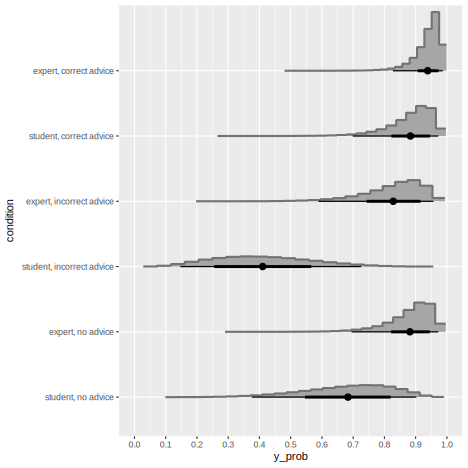
\includegraphics{manuscript_files/figure-pdf/fig-margdist1-1.pdf}

}

\end{figure}%

Figure~\ref{fig-margdist1} shows the model-implied marginal
distributions, including the mean, 66\% and 95\% intervals. We can see
that, indeed, the average probabilities (black dots) slightly differ
from the probabilities of average subjects and items considered
previously. This difference increases with the variability of the random
effects. We can use plots like Figure~\ref{fig-margdist1} as a useful
tool to determine whether the specified standard deviations of the
subject and item random intercepts (\(\sigma_S\) and \(\sigma_I\)) are
reasonable by comparing the ranges and overlap between conditions to
domain knowledge.

\phantomsection\label{cell-fig-margdist2}
\begin{figure}[H]

\caption{\label{fig-margdist2}Marginal distributions including means,
66\% and 95\% confidence intervals for all experimental conditions while
setting the standard deviation of item random intercepts to 0.01.}

\centering{

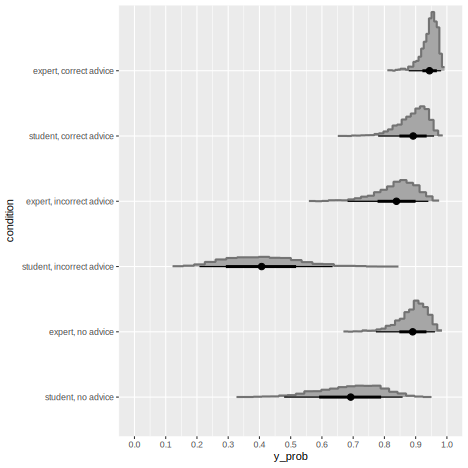
\includegraphics{manuscript_files/figure-pdf/fig-margdist2-1.pdf}

}

\end{figure}%

For the next plot, we have set the item standard deviation to almost
zero (\(\sigma_I = 0.01\)). This gives us a better way to see the
variability between persons. As an example, Figure~\ref{fig-margdist2}
reveals a number of implicit assumptions about the comparison between
experts and students: With incorrect advice, virtually all experts have
a higher probability of making a correct diagnosis compared to students
when considering only items with average difficulty. In contrast, there
is considerable overlap in probability between experts and students with
no advice and even higher overlap with correct advice. Patterns like
these should be considered carefully and discussed with the domain
experts. Parameter values (\(\beta\) parameters, and \(\sigma_S\))
should be adjusted if the implications do not seem reasonable.\\
The final plot demonstrates that these plots are also useful for
spotting standard deviations that were specified too high. For
Figure~\ref{fig-margdist3} we have set \(\sigma_S = 3\) and
\(\sigma_I = 3\). This implies that in each experimental condition, the
probabilities that a subject solves an item are overwhelmingly close to
either 0 or 1 and nothing in between, which is not a plausible
assumption. These high standard deviations do not account for the
inherent variability and complexity of human performance. For example,
the expectation that an expert with low ability and incorrect advice
would solve a difficult item with a probability close to zero is not
convincing.

\phantomsection\label{cell-fig-margdist3}
\begin{figure}[H]

\caption{\label{fig-margdist3}Marginal distributions including means,
66\% and 95\% confidence intervals for all experimental conditions while
setting the standard deviation of subject and item random intercepts to
3.}

\centering{

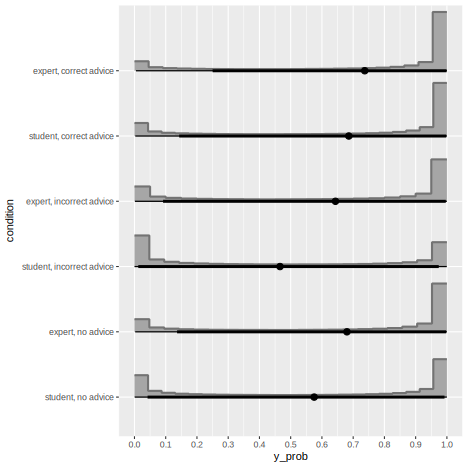
\includegraphics{manuscript_files/figure-pdf/fig-margdist3-1.pdf}

}

\end{figure}%

\subsubsection{Iterate with domain
expertise}\label{iterate-with-domain-expertise}

\subsubsection{THEORY}\label{theory-5}

Tailored simulation-based sample size planning always requires access to
domain knowledge. However, gathering domain knowledge and the
specification of population parameter values is not always
straightforward and can be better described as an iterative process, in
which the plausibility of simulated data is repeatedly compared with the
available domain expertise. As a first step, dedicated domain experts
(if available) can be interviewed to \emph{elicit} their domain
knowledge about how the data of the planned study is expected to look.
Because most domain experts are no experts in statistical modeling and
GLMMs, they often struggle without further guidance to communicate their
knowledge in a way that is useful when specifying the parameters for
data simulation. For this reason, we suggest that after an initial
interview, the analyst who is familiar with the structure of the GLMM
selects an initial set of insightful descriptive statistics and
model-based quantities. Then, they reenter into an iterative discussion
with the domain experts where some set of population values are
selected, and the plausibility of resulting implied quantities is
evaluated. The population parameters are updated until the domain
experts are satisfied with the result. During this process, the
monitored descriptive statistics and model-based quantities can be
updated or extended to capture as much available domain knowledge as
possible. Even if no dedicated domain experts are available, the basic
principles stay the same except that initial parameter values are often
derived from a more extensive literature review. Descriptive statistics
and model-based quantities are still used to evaluate whether the
implied assumptions about the data generating process are plausible.
Often, this judgment evolves over several iterations as the analyst
becomes more familiar with the model and the study design.\footnote{Developing
  more effective strategies on how to elicit and visualize domain
  knowledge is currently an active area of research, primarily in the
  context of Bayesian modeling
  (\citeproc{ref-bocktingSimulationbasedPriorKnowledge2024}{Bockting et
  al., 2024};
  \citeproc{ref-hartmannFlexiblePriorElicitation2020}{Hartmann et al.,
  2020}; \citeproc{ref-mikkolaPriorKnowledgeElicitation2023}{Mikkola et
  al., 2023};
  \citeproc{ref-stefanPracticalChallengesMethodological2022}{Stefan et
  al., 2022}). We expect that future advances in this field will also be
  highly relevant for tailored simulation-based sample size planning
  with frequentist models.}

\subsubsection{PRACTICE}\label{practice-5}

All parameter values in our present case study have been determined
based on repeated discussions with domain experts in radiology to
validate our assumptions. Initially, we reviewed the literature to
establish a reasonable baseline performance rate for examining head CT
scans for intracranial hemorrhage. Existing studies indicate that
radiologists typically demonstrate high accuracies around 90\%, while
interns have been shown to perform below 80\%, and medical students fall
even shorter. For simplicity, we assumed plausible probability values of
.90 for experts and .70 for students, respectively. Our experts
confirmed that these values are realistic baselines for reviewing
diverse head CT images without AI assistance. Subsequently, we consulted
several published papers investigating the effect of correct and
incorrect advice on decision-making performance in other settings. From
their findings, we inferred that both experts and students should
benefit from correct and suffer losses from incorrect advice. However,
the magnitude of these effects should be substantially greater for
students, given their stronger reliance on advice compared to experts.
We further validated the plausibility of our estimated gains and losses
with the collaborating radiologists until we settled on the
probabilities shown in Table 2.

\subsection{Step 4: Estimate the statistical
model}\label{step-4-estimate-the-statistical-model}

\subsubsection{THEORY}\label{theory-6}

At this point, the researcher is capable of producing a simulated
dataset that is comparable to the actual dataset to be collected in the
planned study. The next step is to specify how the statistical model
shall be estimated in the actual study collected later. This requires
the selection of a statistical framework, a software package that is
capable of estimating the model class of interest, an estimation
algorithm, and the specific model structure including all fixed effects,
random effects, and the model family of the dependent variable.

Note that this does not always mean that one will specify the same GLMM
that was used when specifying the data-generating process. On the one
hand, using a simpler model for data simulation than for model
estimation can be a useful strategy in scenarios where making plausible
assumptions for complicated random effect structures and interactions is
not feasible, or the omitted components are expected to have small
effects (\citeproc{ref-matuschekBalancingTypeError2017}{Matuschek et
al., 2017}). On the other hand, using a more complex model for data
simulation than for model estimation can be a useful strategy in
scenarios where one has specific domain knowledge about aspects of the
data-generating process that are still difficult to estimate with the
current state-of-the-art in multilevel modeling. In fact, applying
models that are more parsimonious than the true data generating process
can provide a better trade-off between type I error rates (or bias) and
power (or precision) in many scenarios
(\citeproc{ref-matuschekBalancingTypeError2017}{Matuschek et al.,
2017}).

\subsubsection{PRACTICE}\label{practice-6}

In our case study, we use the \emph{lme4} R package
(\citeproc{ref-batesFittingLinearMixedEffects2015}{Bates et al., 2015}),
which is a state-of-the-art tool for fitting frequentist
GLMMs.\footnote{For Bayesian GLMMs, the \emph{brms} R package is
  currently the most prominent option
  (\citeproc{ref-burknerBrmsPackageBayesian2017}{Bürkner, 2017}).} For
the current example, we simulate data according to our model, in which
100 subjects respond to 50 items (we use \texttt{set.seed} to make the
simulation reproducible). However, for the sake of the exercise, we can
imagine that this would be real data resulting from our future
experiment and think about how we would analyze this data.

\begin{Shaded}
\begin{Highlighting}[]
\FunctionTok{library}\NormalTok{(tidyverse)}
\FunctionTok{set.seed}\NormalTok{(}\DecValTok{1}\NormalTok{)}
\NormalTok{dat }\OtherTok{\textless{}{-}} \FunctionTok{simulate}\NormalTok{(}\AttributeTok{n\_subjects =} \DecValTok{100}\NormalTok{, }\AttributeTok{n\_items =} \DecValTok{50}\NormalTok{)}
\end{Highlighting}
\end{Shaded}

The \emph{lme4} package uses a special syntax for model specification.
Our specific GLMM is represented by the formula:

\begin{Shaded}
\begin{Highlighting}[]
\FunctionTok{library}\NormalTok{(lme4)}
\NormalTok{f }\OtherTok{\textless{}{-}}\NormalTok{ y\_bin }\SpecialCharTok{\textasciitilde{}} \DecValTok{1} \SpecialCharTok{+}\NormalTok{ expert }\SpecialCharTok{+}\NormalTok{ advice\_present }\SpecialCharTok{+}\NormalTok{ advice\_correct }\SpecialCharTok{+} 
\NormalTok{  expert}\SpecialCharTok{:}\NormalTok{advice\_present }\SpecialCharTok{+}\NormalTok{ expert}\SpecialCharTok{:}\NormalTok{advice\_correct }\SpecialCharTok{+}
\NormalTok{  (}\DecValTok{1}\SpecialCharTok{|}\NormalTok{subject) }\SpecialCharTok{+}\NormalTok{ (}\DecValTok{1}\SpecialCharTok{|}\NormalTok{item)}
\end{Highlighting}
\end{Shaded}

The first two lines look similar to any linear model in R (general
intercept indicated by \texttt{1}; main effects indicated by variable
names in the dataset; interactions indicated by
\texttt{variable1:variable2}). The third line specifies a random
intercept for each subject \texttt{(1\textbar{}subject)} and for each
item \texttt{(1\textbar{}item)}. The complete set of rules for the
syntax is outlined in Bates et al.
(\citeproc{ref-batesFittingLinearMixedEffects2015}{2015}) and in the
documentation of the \emph{lme4} package.

In \emph{lme4}, a GLMM is fitted with the \texttt{glmer} function. By
setting \texttt{family\ =\ \ "binomial"}, we request a binomial GLMM
appropriate for our binary dependent variable \texttt{y\_bin} (the
binomial GLMM uses the canonical logit link by default), which is
defined as an accurate (1) vs.~inaccurate (0) diagnosis. We use the
default estimation algorithm (see \texttt{?glmerControl} for a list of
alternative options).

\begin{Shaded}
\begin{Highlighting}[]
\NormalTok{fit }\OtherTok{\textless{}{-}} \FunctionTok{glmer}\NormalTok{(f, }\AttributeTok{data =}\NormalTok{ dat, }\AttributeTok{family =} \StringTok{"binomial"}\NormalTok{)}
\end{Highlighting}
\end{Shaded}

We can inspect the estimates for all model parameters with the
\texttt{summary} command:

\begin{Shaded}
\begin{Highlighting}[]
\FunctionTok{summary}\NormalTok{(fit)}
\end{Highlighting}
\end{Shaded}

\begin{verbatim}
Generalized linear mixed model fit by maximum likelihood (Laplace
  Approximation) [glmerMod]
 Family: binomial  ( logit )
Formula: 
y_bin ~ 1 + expert + advice_present + advice_correct + expert:advice_present +  
    expert:advice_correct + (1 | subject) + (1 | item)
   Data: dat

     AIC      BIC   logLik deviance df.resid 
  4149.4   4201.6  -2066.7   4133.4     4992 

Scaled residuals: 
    Min      1Q  Median      3Q     Max 
-5.7669  0.2125  0.3046  0.4317  2.1056 

Random effects:
 Groups  Name        Variance Std.Dev.
 subject (Intercept) 0.3148   0.5611  
 item    (Intercept) 0.1624   0.4029  
Number of obs: 5000, groups:  subject, 100; item, 50

Fixed effects:
                      Estimate Std. Error z value Pr(>|z|)    
(Intercept)             1.0339     0.1103   9.374  < 2e-16 ***
expert                  1.1849     0.2096   5.654 1.57e-08 ***
advice_present         -1.3436     0.1206 -11.143  < 2e-16 ***
advice_correct          2.6154     0.1273  20.540  < 2e-16 ***
expert:advice_present   1.0589     0.2940   3.601 0.000317 ***
expert:advice_correct  -1.8104     0.2915  -6.210 5.28e-10 ***
---
Signif. codes:  0 '***' 0.001 '**' 0.01 '*' 0.05 '.' 0.1 ' ' 1

Correlation of Fixed Effects:
            (Intr) expert advc_p advc_c exprt:dvc_p
expert      -0.377                                 
advic_prsnt -0.349  0.176                          
advic_crrct  0.023  0.001 -0.668                   
exprt:dvc_p  0.143 -0.448 -0.412  0.276            
exprt:dvc_c -0.008  0.004  0.292 -0.435 -0.686     
\end{verbatim}

In the model output, the \texttt{Estimate} column in the
\texttt{Fixed\ effects} table contains the estimates for the \(\beta\)
parameters, while the \texttt{Std.Dev.} column in the
\texttt{Random\ effects} table contains the estimates for \(\sigma_S\)
and \(\sigma_I\).

\subsection{Step 5: Compute the
estimate}\label{step-5-compute-the-estimate}

\subsubsection{THEORY}\label{theory-7}

In previous steps, we have defined the theoretical estimand, written a
data simulation function and specified how to estimate a GLMM using
simulated data. The next step is to specify how to compute a concrete
point estimate of the theoretical estimand within the framework of the
fitted GLMM. For some research questions, the estimate corresponds with
a single regression coefficient. In more complicated scenarios, the
estimate is computed from a combination of coefficients. Beyond
computing the point estimate, we have already discussed that both
hypothesis testing and interval estimation could be used to answer the
research question. The decision on testing or estimating is then
followed by selecting the specific statistical method that shall be
applied to compute the HTs or CIs (e.g., compute HTs and CIs with the
\emph{marginaleffects} R package using the delta method).

\subsubsection{PRACTICE}\label{practice-7}

In the estimand section, we have translated a verbal description of our
research question into four probability statements that are specified
outside of any specific statistical model. For a concrete estimate
within the context of our specified GLMM, we must compute the following
probability contrasts:

\[
\begin{aligned}
& P(Y=1|advice\_present = 1, advice\_correct = 1, expert = 1, u_{0s} = 0, u_{0i} = 0) \\
& \quad - P(Y=1|advice\_present = 0, advice\_correct = 0, expert = 1, u_{0s} = 0, u_{0i} = 0)
\end{aligned}
\] \[
\begin{aligned}
& P(Y=1|advice\_present = 0, advice\_correct = 0, expert = 1, u_{0s} = 0, u_{0i} = 0) \\
& \quad - P(Y=1|advice\_present = 1, advice\_correct = 0, expert = 1, u_{0s} = 0, u_{0i} = 0)
\end{aligned}
\]

\[
\begin{aligned}
& P(Y=1|advice\_present = 1, advice\_correct = 1, expert = 0, u_{0s} = 0, u_{0i} = 0) \\
& \quad - P(Y=1|advice\_present = 0, advice\_correct = 0, expert = 0, u_{0s} = 0, u_{0i} = 0)
\end{aligned}
\]

\[
\begin{aligned}
& P(Y=1|advice\_present = 0, advice\_correct = 0, expert = 0, u_{0s} = 0, u_{0i} = 0) \\
& \quad - P(Y=1|advice\_present = 1, advice\_correct = 0, expert = 0, u_{0s} = 0, u_{0i} = 0)
\end{aligned}
\] We have already discussed how to compute the involved probabilities
in the section on specifying population parameters. Plugging in the GLMM
model equation produces an equation for computing each contrast if all
model parameters were known. When we want to estimate the above
contrasts based on observed data, the only difference is that model
parameters are not known and we instead use the corresponding parameter
estimates.

We could use our knowledge of the structure of the GLMM to determine the
exact formula needed to compute the contrasts of interest and then plug
in the parameter estimates manually from the \texttt{summary(fit)}
output. However, this would be tedious and we can use R to compute this
contrast without doing the math. Using the first contrast \emph{(correct
advice, expert) - (no advice, expert)} as our example, we could apply
the \texttt{predict} function of the \emph{lme4} package to compute the
predicted probability for a correct diagnosis based on our fitted model,
plug in the two sets of predictor values, and compute the difference
between the two estimated probabilities.

\begin{Shaded}
\begin{Highlighting}[]
\NormalTok{grid1 }\OtherTok{\textless{}{-}} \FunctionTok{data.frame}\NormalTok{(}\AttributeTok{advice\_present =} \FunctionTok{c}\NormalTok{(}\DecValTok{1}\NormalTok{, }\DecValTok{0}\NormalTok{), }\AttributeTok{advice\_correct =} \FunctionTok{c}\NormalTok{(}\DecValTok{1}\NormalTok{, }\DecValTok{0}\NormalTok{), }
  \AttributeTok{expert =} \FunctionTok{c}\NormalTok{(}\DecValTok{1}\NormalTok{, }\DecValTok{1}\NormalTok{))}
\NormalTok{grid1}
\end{Highlighting}
\end{Shaded}

\begin{verbatim}
  advice_present advice_correct expert
1              1              1      1
2              0              0      1
\end{verbatim}

\begin{Shaded}
\begin{Highlighting}[]
\NormalTok{pred }\OtherTok{\textless{}{-}} \FunctionTok{predict}\NormalTok{(fit, }\AttributeTok{newdata =}\NormalTok{ grid1, }\AttributeTok{type =} \StringTok{"response"}\NormalTok{, }\AttributeTok{re.form =} \ConstantTok{NA}\NormalTok{)}
\NormalTok{pred}
\end{Highlighting}
\end{Shaded}

\begin{verbatim}
       1        2 
0.939292 0.901923 
\end{verbatim}

\begin{Shaded}
\begin{Highlighting}[]
\NormalTok{pred[}\DecValTok{1}\NormalTok{] }\SpecialCharTok{{-}}\NormalTok{ pred[}\DecValTok{2}\NormalTok{]}
\end{Highlighting}
\end{Shaded}

\begin{verbatim}
         1 
0.03736901 
\end{verbatim}

The argument \texttt{type\ =\ "response"} specifies that predictions are
made on the probability scale (instead of the log-odds scale of the
\(\beta\) parameters), while \texttt{re.form\ =\ NA} sets all random
effects to 0. We could use this method to compute point estimates for
all four contrasts that are part of our estimand. However, depending on
whether we are interested in hypothesis testing or parameter estimation,
we also need a method to compute HTs or CIs. The \emph{marginaleffects}
package (\citeproc{ref-R-marginaleffects}{Arel-Bundock et al.,
Forthcoming}) is a very flexible, increasingly popular package to
compute HTs and CIs for contrasts with a variety of statistical models,
including GLMMs estimated with \emph{lme4}. First, we specify a grid of
all combinations of predictor variables and then compute estimated
probabilities for all experimental conditions in our experiment with the
\texttt{predictions} function:

\begin{Shaded}
\begin{Highlighting}[]
\FunctionTok{library}\NormalTok{(tidyverse)}
\FunctionTok{library}\NormalTok{(marginaleffects)}
\FunctionTok{library}\NormalTok{(tinytable)}
\NormalTok{grid2 }\OtherTok{\textless{}{-}} \FunctionTok{expand\_grid}\NormalTok{(}\AttributeTok{advice\_present =} \DecValTok{0}\SpecialCharTok{:}\DecValTok{1}\NormalTok{, }
  \AttributeTok{advice\_correct =} \DecValTok{0}\SpecialCharTok{:}\DecValTok{1}\NormalTok{, }\AttributeTok{expert =} \DecValTok{0}\SpecialCharTok{:}\DecValTok{1}\NormalTok{)}
\NormalTok{grid2}
\end{Highlighting}
\end{Shaded}

\begin{verbatim}
# A tibble: 8 x 3
  advice_present advice_correct expert
           <int>          <int>  <int>
1              0              0      0
2              0              0      1
3              0              1      0
4              0              1      1
5              1              0      0
6              1              0      1
7              1              1      0
8              1              1      1
\end{verbatim}

\begin{Shaded}
\begin{Highlighting}[]
\NormalTok{preds }\OtherTok{\textless{}{-}} \FunctionTok{predictions}\NormalTok{(fit, }\AttributeTok{newdata =}\NormalTok{ grid2, }
  \AttributeTok{type =} \StringTok{"response"}\NormalTok{, }\AttributeTok{re.form =} \ConstantTok{NA}\NormalTok{)}
\FunctionTok{print}\NormalTok{(preds, }\AttributeTok{style =} \StringTok{"tinytable"}\NormalTok{) }\SpecialCharTok{\%\textgreater{}\%} \FunctionTok{theme\_tt}\NormalTok{(}\AttributeTok{theme =} \StringTok{"resize"}\NormalTok{)}
\end{Highlighting}
\end{Shaded}

\begin{table}
\centering
\resizebox{\ifdim\width>\linewidth 1\linewidth\else\width\fi}{!}{
\begin{talltblr}[         %% tabularray outer open
entry=none,label=none,
note{}={Type:  response 
},
note{ }={Columns: rowid, estimate, std.error, statistic, p.value, s.value, conf.low, conf.high, advice\_present, advice\_correct, expert, y\_bin 
},
]                     %% tabularray outer close
{                     %% tabularray inner open
colspec={Q[]Q[]Q[]Q[]Q[]Q[]Q[]Q[]Q[]Q[]},
}                     %% tabularray inner close
\toprule
Estimate & Std. Error & z & Pr(>|z|) & S & 2.5 \% & 97.5 \% & advice\_present & advice\_correct & expert \\ \midrule %% TinyTableHeader
0.738 & 0.02134 &  34.6 & <0.001 & 867.2 & 0.696 & 0.779 & 0 & 0 & 0 \\
0.902 & 0.01739 &  51.9 & <0.001 & Inf & 0.868 & 0.936 & 0 & 0 & 1 \\
0.975 & 0.00421 & 231.6 & <0.001 & Inf & 0.966 & 0.983 & 0 & 1 & 0 \\
0.954 & 0.01454 &  65.6 & <0.001 & Inf & 0.925 & 0.982 & 0 & 1 & 1 \\
0.423 & 0.03221 &  13.1 & <0.001 & 128.6 & 0.360 & 0.486 & 1 & 0 & 0 \\
0.874 & 0.02793 &  31.3 & <0.001 & 711.4 & 0.819 & 0.928 & 1 & 0 & 1 \\
0.909 & 0.00967 &  94.1 & <0.001 & Inf & 0.890 & 0.928 & 1 & 1 & 0 \\
0.939 & 0.01091 &  86.1 & <0.001 & Inf & 0.918 & 0.961 & 1 & 1 & 1 \\
\bottomrule
\end{talltblr}
}
\end{table}

The point estimates for all experimental conditions are reported in the
\texttt{Estimate} column. Note that the output also contains the two
missing by design conditions that will never be observed in the actual
study (\(advice\_present = 0, advice\_correct = 1, expert = 1\) and
\(advice\_present = 0, advice\_correct = 1, expert = 0\)). This is no
problem as long as we never interpret those estimates. Next, we use the
estimated probabilities to compute the four specific contrasts that are
part of our estimand. For this, we must specify which rows in
\texttt{preds} have to be subtracted from each other. We will use the
\texttt{hypotheses} function to compute our four contrasts of interest
together with HTs and CIs. We use the default inference options of the
\emph{marginaleffects} package that compute HTs and CIs based on the
approximate delta method.

\begin{Shaded}
\begin{Highlighting}[]
\NormalTok{contrasts }\OtherTok{\textless{}{-}}\NormalTok{ preds }\SpecialCharTok{\%\textgreater{}\%} 
  \FunctionTok{hypotheses}\NormalTok{(}\AttributeTok{hypothesis =} \FunctionTok{c}\NormalTok{(}
    \StringTok{"b8 = b2"}\NormalTok{,  }\CommentTok{\# (correct advice, expert) {-} (no advice, expert)}
    \StringTok{"b2 = b6"}\NormalTok{,  }\CommentTok{\# (no advice, expert) {-} (incorrect advice, expert) }
    \StringTok{"b7 = b1"}\NormalTok{,  }\CommentTok{\# (correct advice, student) {-} (no advice, student)}
    \StringTok{"b1 = b5"}\NormalTok{), }\CommentTok{\# (no advice, student) {-} (incorrect advice, student)}
    \AttributeTok{equivalence =} \FunctionTok{c}\NormalTok{(}\DecValTok{0}\NormalTok{, }\DecValTok{0}\NormalTok{))}
\FunctionTok{print}\NormalTok{(contrasts, }\AttributeTok{style =} \StringTok{"tinytable"}\NormalTok{) }\SpecialCharTok{\%\textgreater{}\%} \FunctionTok{theme\_tt}\NormalTok{(}\AttributeTok{theme =} \StringTok{"resize"}\NormalTok{)}
\end{Highlighting}
\end{Shaded}

\begin{table}
\centering
\resizebox{\ifdim\width>\linewidth 1\linewidth\else\width\fi}{!}{
\begin{talltblr}[         %% tabularray outer open
entry=none,label=none,
note{}={Type:  response 
},
note{ }={Columns: term, estimate, std.error, statistic, p.value, s.value, conf.low, conf.high, statistic.noninf, statistic.nonsup, p.value.noninf, p.value.nonsup, p.value.equiv 
},
]                     %% tabularray outer close
{                     %% tabularray inner open
colspec={Q[]Q[]Q[]Q[]Q[]Q[]Q[]Q[]Q[]Q[]Q[]},
}                     %% tabularray inner close
\toprule
Term & Estimate & Std. Error & z & Pr(>|z|) & S & 2.5 \% & 97.5 \% & p (NonSup) & p (NonInf) & p (Equiv) \\ \midrule %% TinyTableHeader
b8=b2 & 0.0374 & 0.0162 &  2.31 & 0.021 & 5.6 &  0.00563 & 0.0691 & 0.989 & 0.0105 & 0.989 \\
b2=b6 & 0.0282 & 0.0279 &  1.01 & 0.312 & 1.7 & -0.02653 & 0.0830 & 0.844 & 0.1562 & 0.844 \\
b7=b1 & 0.1717 & 0.0173 &  9.93 & <0.001 & 74.8 &  0.13780 & 0.2056 & 1.000 & <0.001 & 1.000 \\
b1=b5 & 0.3145 & 0.0280 & 11.24 & <0.001 & 95.0 &  0.25965 & 0.3693 & 1.000 & <0.001 & 1.000 \\
\bottomrule
\end{talltblr}
}
\end{table}

The expression \texttt{"b8\ =\ b2"} is special syntax to subtract the
estimate in row number 8 from the estimate in row number 2 in the
\texttt{preds}-output. The argument \texttt{equivalence\ =\ c(0,\ 0)}
can be used to compute one-sided p-values, testing whether the contrast
in the population is smaller than 0 (\texttt{p\ (NonSub)} column) or
greater than 0 (\texttt{p\ (NonInf)} column). The point estimates for
four contrasts are reported in the \texttt{Estimate} column. Note that
to facilitate interpretation, we arranged the contrasts in a way that we
theoretically expect positive values for all four of them.

\textbf{Hypothesis testing.} If we chose hypothesis testing for our case
study, we would test a combined null hypothesis \(H_0\) that consists of
four separate null hypotheses: \[
\begin{aligned}
H_{01}:\ & P(Y=1|advice\_present = 1, advice\_correct = 1, expert = 1, u_{0s} = 0, u_{0i} = 0) \leq \\
& P(Y=1|advice\_present = 0, advice\_correct = 0, expert = 1, u_{0s} = 0, u_{0i} = 0) \\
H_{02}:\ &P(Y=1|advice\_present = 0, advice\_correct = 0, expert = 1, u_{0s} = 0, u_{0i} = 0) \leq \\
& P(Y=1|advice\_present = 1, advice\_correct = 0, expert = 1, u_{0s} = 0, u_{0i} = 0) \\
H_{03}:\ &P(Y=1|advice\_present = 1, advice\_correct = 1, expert = 0, u_{0s} = 0, u_{0i} = 0) \leq \\
& P(Y=1|advice\_present = 0, advice\_correct = 0, expert = 0, u_{0s} = 0, u_{0i} = 0) \\
H_{04}:\ & P(Y=1|advice\_present = 0, advice\_correct = 0, expert = 0, u_{0s} = 0, u_{0i} = 0) \leq \\
& P(Y=1|advice\_present = 1, advice\_correct = 0, expert = 0, u_{0s} = 0, u_{0i} = 0)
\end{aligned}
\] The combined null hypothesis \(H_0\) should only be rejected if
\textbf{all} individual null hypotheses are rejected (i.e.,
intersection-union setting;
\citeproc{ref-dmitrienkoTraditionalMultiplicityAdjustment2013}{Dmitrienko
\& D'Agostino, 2013}). In such cases, the error probabilities do not
accumulate, and we would waste power when correcting for multiple tests.

With a standard significance level of \(\alpha = 0.05\), we would not
reject all four null hypotheses (the p-value in the \texttt{p\ (NonInf)}
column for the second hypothesis is not significant) and therefore also
not reject the combined null hypothesis for this particular (simulated)
dataset. Note that this decision would be wrong because we have
simulated the data such that the combined alternative hypothesis \(H_1\)
is actually true in the population.

\textbf{Interval estimation.} If we chose parameter estimation for our
case study, we would focus on the two-sided CIs of the four contrasts of
interest. With a standard confidence level of \(1 - \alpha = 0.95\)
plausible values are clearly in the positive range for the first, third,
and fourth contrast, while both negative and positive values seem
plausible for the second contrast. Note that due to the constrained
range of the probability scale, the width of the CI differs between the
four contrasts (which is the expected behavior for binomial GLMMs). The
smallest width is observed for the first contrast (expert with correct
advice vs.~expert without advice), where both underlying probabilities
are close to 1. The largest width is observed for the fourth contrast
(student with incorrect advice vs.~student without advice), where both
underlying probabilities are closer to 0.5.

\subsection{Step 6: Perform repeated
simulations}\label{step-6-perform-repeated-simulations}

\subsubsection{THEORY}\label{theory-8}

Conducting all previous steps enables the analyst to 1) simulate a
dataset, 2) estimate a GLMM, and 3) compute HTs or CIs for estimands of
interest, mirroring the analysis that will later be conducted on the
actual dataset of the planned study. To produce an estimate of power or
precision, the last step is to perform these previous steps repeatedly.
On a conceptual level, we first require a function that takes a sample
size and a full set of population parameter values as input. When
planning for power, the function should return the p-value(s) of the
HT(s) of interest when conducted on the simulated dataset. When planning
for precision, the function should return the width of the CI(s) of
interest. Second, we run this function repeatedly with the same sample
size and population parameters. Because fitting GLMMs can quickly become
time-consuming, it is recommended to use parallel computing, that is
running simulations on multiple cores of the computer at the same time
to reduce total run time. Third, the results of the repeated simulation
are collected and aggregated. When planning for power, we compute the
relative frequency of (a) significant p-value(s) across repeated
simulations. When planning for precision, we compute the average width
of the CI(s). Finally, we repeat the complete simulation for different
sample sizes to determine how big the sample must be in order to achieve
the targeted power or precision.

\subsubsection{PRACTICE}\label{practice-8}

Wrapping the \texttt{simulate} function already constructed earlier, the
helper function \texttt{sim\_and\_analyse} performs all previous steps
(simulate a dataset, fit a GLMM, compute p-values and CIs) in a single
command.

\begin{Shaded}
\begin{Highlighting}[]
\NormalTok{sim\_and\_analyse }\OtherTok{\textless{}{-}} \ControlFlowTok{function}\NormalTok{(}
  \AttributeTok{formula\_chr =} \StringTok{"y\_bin \textasciitilde{} 1 + expert + advice\_present + advice\_correct + }
\StringTok{    expert:advice\_present + expert:advice\_correct + (1|subject) + (1|item)"}\NormalTok{,}
  \AttributeTok{contrasts =} \FunctionTok{c}\NormalTok{(}\StringTok{"b8 = b2"}\NormalTok{, }\StringTok{"b2 = b6"}\NormalTok{, }\StringTok{"b7 = b1"}\NormalTok{, }\StringTok{"b1 = b5"}\NormalTok{), ...)\{}
  \FunctionTok{require}\NormalTok{(lme4)}
  \FunctionTok{require}\NormalTok{(marginaleffects)}
  \FunctionTok{require}\NormalTok{(tidyr)}
  \CommentTok{\# simulate data}
\NormalTok{  dat }\OtherTok{\textless{}{-}} \FunctionTok{simulate}\NormalTok{(...)}
  \CommentTok{\# fit model}
\NormalTok{  model }\OtherTok{\textless{}{-}} \FunctionTok{glmer}\NormalTok{(}\FunctionTok{as.formula}\NormalTok{(formula\_chr), }\AttributeTok{data =}\NormalTok{ dat, }\AttributeTok{family =} \StringTok{"binomial"}\NormalTok{)}
  \CommentTok{\# compute contrasts}
\NormalTok{  contr\_df }\OtherTok{\textless{}{-}} \FunctionTok{expand\_grid}\NormalTok{(}\AttributeTok{advice\_present =} \DecValTok{0}\SpecialCharTok{:}\DecValTok{1}\NormalTok{, }\AttributeTok{advice\_correct =} \DecValTok{0}\SpecialCharTok{:}\DecValTok{1}\NormalTok{,}
    \AttributeTok{expert =} \DecValTok{0}\SpecialCharTok{:}\DecValTok{1}\NormalTok{)}
  \FunctionTok{predictions}\NormalTok{(model, }\AttributeTok{newdata =}\NormalTok{ contr\_df, }\AttributeTok{type =} \StringTok{"response"}\NormalTok{, }\AttributeTok{re.form =} \ConstantTok{NA}\NormalTok{) }\SpecialCharTok{\%\textgreater{}\%}
    \FunctionTok{hypotheses}\NormalTok{(}\AttributeTok{hypothesis =}\NormalTok{ contrasts, }\AttributeTok{equivalence =} \FunctionTok{c}\NormalTok{(}\DecValTok{0}\NormalTok{, }\DecValTok{0}\NormalTok{)) }\SpecialCharTok{\%\textgreater{}\%}
    \FunctionTok{data.frame}\NormalTok{()}
\NormalTok{\}}
\end{Highlighting}
\end{Shaded}

We use the \emph{future} (\citeproc{ref-R-RJ-2021-048}{Bengtsson, 2021})
and \emph{furrr} (\citeproc{ref-R-furrr}{Vaughan \& Dancho, 2022})
packages to perform computations in parallel. First, we enable
parallelization with the \texttt{plan} function and specify how many
parallel cores (``workers'') of our computer to use (users can find out
the maximum number of cores on their computer with the command
\texttt{parallel::detectCores()}), and set a seed to make the simulation
reproducible.

\begin{Shaded}
\begin{Highlighting}[]
\FunctionTok{library}\NormalTok{(future)}
\FunctionTok{plan}\NormalTok{(}\StringTok{"multisession"}\NormalTok{, }\AttributeTok{workers =} \DecValTok{6}\NormalTok{)}
\FunctionTok{set.seed}\NormalTok{(}\DecValTok{2}\NormalTok{)}
\end{Highlighting}
\end{Shaded}

The next code chunk specifies a simulation grid with different settings
for both the number of subjects (\texttt{n\_subjects}) and the number of
items (\texttt{n\_items}), each combination being repeated \texttt{rep}
times. The more repetitions, the more accurately power and precision can
be estimated. We chose 300 repetitions for the data simulation at hand
to strike a balance between achieving a robust estimate and remaining
computationally feasible. With the current settings, this simulation
takes several hours on a MacBook Pro from 2020 with M1 chip and 16 GB
working memory. If you want to quickly experiment with the code
yourself, a setting with \texttt{workers\ =\ 4} and \texttt{rep\ =\ 5}
should finish in less than 5 minutes, even on smaller machines.

\begin{Shaded}
\begin{Highlighting}[]
\FunctionTok{library}\NormalTok{(furrr)}
\NormalTok{sim\_result }\OtherTok{\textless{}{-}} \FunctionTok{crossing}\NormalTok{(}
  \AttributeTok{rep =} \DecValTok{1}\SpecialCharTok{:}\DecValTok{500}\NormalTok{,}
  \AttributeTok{n\_subjects =} \FunctionTok{c}\NormalTok{(}\DecValTok{100}\NormalTok{, }\DecValTok{150}\NormalTok{, }\DecValTok{200}\NormalTok{, }\DecValTok{250}\NormalTok{),}
  \AttributeTok{n\_items =} \FunctionTok{c}\NormalTok{(}\DecValTok{10}\NormalTok{, }\DecValTok{30}\NormalTok{, }\DecValTok{50}\NormalTok{, }\DecValTok{70}\NormalTok{)}
\NormalTok{) }\SpecialCharTok{\%\textgreater{}\%}
  \FunctionTok{mutate}\NormalTok{(}\AttributeTok{res =} \FunctionTok{future\_pmap}\NormalTok{(., sim\_and\_analyse, }
    \AttributeTok{.options =} \FunctionTok{furrr\_options}\NormalTok{(}\AttributeTok{seed =} \ConstantTok{TRUE}\NormalTok{))) }\SpecialCharTok{\%\textgreater{}\%}
  \FunctionTok{unnest}\NormalTok{(}\AttributeTok{col =}\NormalTok{ res)}
\end{Highlighting}
\end{Shaded}

The result of this computation is a data frame that contains the
p-values and CIs of all specified contrasts for each simulated dataset.
In some iterations (predominantly in conditions with small sample
sizes), model estimation did not converge with the \emph{lme4} package.
When the model fails to converge, it means that the statistical model
being fitted to the data failed to reach a stable or valid solution
during the estimation process. We do not remove these results because
non-convergence can also happen when analyzing the real data we plan to
collect, thus, we want to factor in this possibility to keep our
simulation more realistic.

\textbf{Power results.} For our exemplary combined hypothesis, power is
defined as the (long-run) percentage of simulations in which all four
p-values of our individual hypotheses are significant at the
\(\alpha = 0.05\) level. Based on our simulation outcomes, we compute a
power estimate for each combination of \texttt{n\_subjects} \(\times\)
\texttt{n\_items} (including 95\% CIs) and visualize the results with
the following code.\footnote{This code was inspired by the ``Mixed
  Design Simulation'' vignette of the \emph{faux} package at
  \url{https://debruine.github.io/faux/articles/sim_mixed.html}.}

\phantomsection\label{cell-fig-finalpwr}
\begin{Shaded}
\begin{Highlighting}[]
\FunctionTok{library}\NormalTok{(binom)}
\NormalTok{alpha }\OtherTok{\textless{}{-}} \FloatTok{0.05}
\NormalTok{power }\OtherTok{\textless{}{-}}\NormalTok{ sim\_result }\SpecialCharTok{\%\textgreater{}\%}
  \FunctionTok{pivot\_wider}\NormalTok{(}\AttributeTok{names\_from =}\NormalTok{ term, }\AttributeTok{names\_sep =} \StringTok{"\_"}\NormalTok{, }
    \AttributeTok{values\_from =}\NormalTok{ estimate}\SpecialCharTok{:}\NormalTok{p.value.equiv) }\SpecialCharTok{\%\textgreater{}\%}
  \FunctionTok{group\_by}\NormalTok{(n\_subjects, n\_items) }\SpecialCharTok{\%\textgreater{}\%} 
  \FunctionTok{summarise}\NormalTok{(}
    \AttributeTok{power =} \FunctionTok{mean}\NormalTok{(}\StringTok{\textasciigrave{}}\AttributeTok{p.value.noninf\_b1=b5}\StringTok{\textasciigrave{}} \SpecialCharTok{\textless{}}\NormalTok{ alpha }\SpecialCharTok{\&} 
        \StringTok{\textasciigrave{}}\AttributeTok{p.value.noninf\_b8=b2}\StringTok{\textasciigrave{}} \SpecialCharTok{\textless{}}\NormalTok{ alpha }\SpecialCharTok{\&} \StringTok{\textasciigrave{}}\AttributeTok{p.value.noninf\_b2=b6}\StringTok{\textasciigrave{}} \SpecialCharTok{\textless{}}\NormalTok{ alpha }\SpecialCharTok{\&} 
        \StringTok{\textasciigrave{}}\AttributeTok{p.value.noninf\_b7=b1}\StringTok{\textasciigrave{}} \SpecialCharTok{\textless{}}\NormalTok{ alpha), }
    \AttributeTok{n\_sig =} \FunctionTok{sum}\NormalTok{(}\StringTok{\textasciigrave{}}\AttributeTok{p.value.noninf\_b1=b5}\StringTok{\textasciigrave{}} \SpecialCharTok{\textless{}}\NormalTok{ alpha }\SpecialCharTok{\&} 
        \StringTok{\textasciigrave{}}\AttributeTok{p.value.noninf\_b8=b2}\StringTok{\textasciigrave{}} \SpecialCharTok{\textless{}}\NormalTok{ alpha }\SpecialCharTok{\&} \StringTok{\textasciigrave{}}\AttributeTok{p.value.noninf\_b2=b6}\StringTok{\textasciigrave{}} \SpecialCharTok{\textless{}}\NormalTok{ alpha }\SpecialCharTok{\&} 
        \StringTok{\textasciigrave{}}\AttributeTok{p.value.noninf\_b7=b1}\StringTok{\textasciigrave{}} \SpecialCharTok{\textless{}}\NormalTok{ alpha),}
    \AttributeTok{n =} \FunctionTok{n}\NormalTok{(),}
    \AttributeTok{ci.lwr =} \FunctionTok{binom.confint}\NormalTok{(n\_sig, n, }\AttributeTok{method =} \StringTok{"wilson"}\NormalTok{)}\SpecialCharTok{$}\NormalTok{lower,}
    \AttributeTok{ci.upr =} \FunctionTok{binom.confint}\NormalTok{(n\_sig, n, }\AttributeTok{method =} \StringTok{"wilson"}\NormalTok{)}\SpecialCharTok{$}\NormalTok{upper, }
    \AttributeTok{.groups =} \StringTok{"drop"}\NormalTok{)}
\NormalTok{power }\SpecialCharTok{\%\textgreater{}\%}
  \FunctionTok{mutate}\NormalTok{(}\FunctionTok{across}\NormalTok{(}\FunctionTok{c}\NormalTok{(n\_subjects, n\_items), factor)) }\SpecialCharTok{\%\textgreater{}\%}
  \FunctionTok{ggplot}\NormalTok{(}\FunctionTok{aes}\NormalTok{(n\_subjects, n\_items, }\AttributeTok{fill =}\NormalTok{ power)) }\SpecialCharTok{+}
  \FunctionTok{geom\_tile}\NormalTok{() }\SpecialCharTok{+}
  \FunctionTok{geom\_text}\NormalTok{(}\FunctionTok{aes}\NormalTok{(}\AttributeTok{label =} \FunctionTok{sprintf}\NormalTok{(}\StringTok{"\%.2f }\SpecialCharTok{\textbackslash{}n}\StringTok{ [\%.2f; \%.2f]"}\NormalTok{, }
\NormalTok{                                power, ci.lwr, ci.upr)), }
    \AttributeTok{color =} \StringTok{"white"}\NormalTok{, }\AttributeTok{size =} \DecValTok{4}\NormalTok{) }\SpecialCharTok{+}
  \FunctionTok{scale\_fill\_viridis\_c}\NormalTok{(}\AttributeTok{limits =} \FunctionTok{c}\NormalTok{(}\DecValTok{0}\NormalTok{, }\DecValTok{1}\NormalTok{)) }\SpecialCharTok{+}
  \FunctionTok{xlab}\NormalTok{(}\StringTok{"number of subjects"}\NormalTok{) }\SpecialCharTok{+} \FunctionTok{ylab}\NormalTok{(}\StringTok{"number of items"}\NormalTok{)}
\end{Highlighting}
\end{Shaded}

\begin{figure}[H]

\caption{\label{fig-finalpwr}Simulation-based power estimates including
95\% confidence interval of the case study for different numbers of
subjects and items, based on a significance level of 0.05.}

\centering{

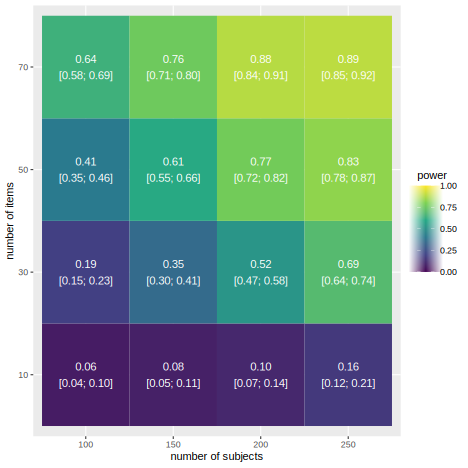
\includegraphics{manuscript_files/figure-pdf/fig-finalpwr-1.pdf}

}

\end{figure}%

As should be the case, power estimates in Figure~\ref{fig-finalpwr}
increase with both the number of subjects and the number of items. The
CIs reported here indicate how precisely power was estimated by our
simulation. Higher precision (which would be reflected in narrower CIs)
could be obtained by increasing the number of repetitions (\texttt{rep})
in the simulation. In practice, data simulations are often run multiple
times with adjusted combinations of sample sizes. When running for the
first time, it might be revealed that power is way too low (or much
higher than required) for some combinations of \texttt{n\_subjects} and
\texttt{n\_items}. When narrowing down the best combination that
achieves sufficient power while at the same time striking a good balance
of how many subjects and items are practically feasible, later rounds of
data simulation will typically include a smaller grid of sample sizes
combined with a higher number of repetitions. This will assure high
precision for the final power estimates, which are then used for the
sample size justification of the planned study.

When target power has been specified, the number of subjects and the
number of items in our study design can be traded against each other
based on practical considerations. Although it is recommended to justify
the power (\citeproc{ref-lakensSampleSizeJustification2022}{Lakens,
2022a}), we adopt the common heuristic to target a power of 0.8 to
detect an effect of the expected size implied by our data simulation.
This could be achieved by collecting data from 250 subjects (about 25\%
of which will be experts), each completing the same 50 items (with
advice present in about 67\% of cases, which is correct in about 80\% of
cases with present advice). If collecting data from 250 subjects is not
feasible, an alternative would be to recruit 200 subjects but increase
the length of the experiment to 70 items. However, 70 items might take
too long to complete for the radiologists participating in the study,
who have a busy schedule. The simulation suggests that it might also be
possible to plan a shorter experiment with only 30 items if it is
feasible to recruit an even higher number of subjects (to be determined
by additional rounds of power analysis). Design parameters that also
affect power, and which could be investigated in the simulation to find
a more optimal trade-off, are the ratio of experts to students, the
frequency of whether advice is presented at all, and whether it is
correct or incorrect.\footnote{An advanced alternative to our heuristic
  trade-off between subjects and items would be to explicitly optimize
  for cost-efficient study designs using the \emph{mlpwr} package
  (\citeproc{ref-zimmerSampleSizePlanning2023}{Zimmer et al., 2023}).
  The package performs simulation-based power analysis in a surrogate
  modeling framework that can evaluate power for a large grid of design
  combinations more efficiently. The framework also requires users to
  write their own \texttt{sim\_and\_analyse} function and can be
  considered a great extension on what we cover in our tutorial.}

\textbf{Precision results.} When planning for precision, one could
monitor the width of all four CIs at the same time. However, because the
CIs of the four contrasts strongly differ in width, it is not trivial to
decide which width one should target when deciding on the appropriate
sample size. In contrast to planning for power, there are no common
standards on how to specify the targeted precision
(\citeproc{ref-lakensSampleSizeJustification2022}{Lakens, 2022a}). For
our example, we use a simple heuristic but we strongly encourage readers
to think about better alternatives that are appropriate in their own
applications. Our simulations show that the smallest CI can be expected
for the first contrast (expert with correct advice vs.~expert without
advice). The true contrast in probability for an average expert and an
average item in this condition is
\texttt{plogis(b\_0\ +\ b\_e\ +\ b\_a\ +\ b\_c\ +\ b\_ea\ +\ b\_ec)\ -\ plogis(b\_0\ +\ b\_e)\ =}
\(0.05\). We want the width of this CI to be smaller than 0.1. This
would mean that if the point estimate happens to be close to the true
value, the plausible values inside of a 95\% CI would all be positive.

Thus in our example, precision is defined as the (long-run) average
width of a 95\% CI for the probability contrast between experts with
correct advice and experts without advice. Of course, a lower width
implies better precision. Based on our simulation outcomes, we compute
the precision estimate for each combination of \texttt{n\_subjects}
\(\times\) \texttt{n\_items} (including 95\% CIs) and visualize the
results with the following code.

\phantomsection\label{cell-fig-finalprecision}
\begin{Shaded}
\begin{Highlighting}[]
\NormalTok{precision }\OtherTok{\textless{}{-}}\NormalTok{ sim\_result }\SpecialCharTok{\%\textgreater{}\%}
  \FunctionTok{pivot\_wider}\NormalTok{(}\AttributeTok{names\_from =}\NormalTok{ term, }\AttributeTok{names\_sep =} \StringTok{"\_"}\NormalTok{, }
    \AttributeTok{values\_from =}\NormalTok{ estimate}\SpecialCharTok{:}\NormalTok{p.value.equiv) }\SpecialCharTok{\%\textgreater{}\%}
  \FunctionTok{group\_by}\NormalTok{(n\_subjects, n\_items) }\SpecialCharTok{\%\textgreater{}\%}
  \FunctionTok{mutate}\NormalTok{(}\AttributeTok{width =} \StringTok{\textasciigrave{}}\AttributeTok{conf.high\_b8=b2}\StringTok{\textasciigrave{}} \SpecialCharTok{{-}} \StringTok{\textasciigrave{}}\AttributeTok{conf.low\_b8=b2}\StringTok{\textasciigrave{}}\NormalTok{) }\SpecialCharTok{\%\textgreater{}\%}
  \FunctionTok{summarise}\NormalTok{(}\AttributeTok{precision =} \FunctionTok{mean}\NormalTok{(width),}
    \AttributeTok{ci.lwr =} \FunctionTok{t.test}\NormalTok{(width)}\SpecialCharTok{$}\NormalTok{conf.int[}\DecValTok{1}\NormalTok{],}
    \AttributeTok{ci.upr =} \FunctionTok{t.test}\NormalTok{(width)}\SpecialCharTok{$}\NormalTok{conf.int[}\DecValTok{2}\NormalTok{], }
    \AttributeTok{.groups =} \StringTok{"drop"}\NormalTok{)}
\NormalTok{precision }\SpecialCharTok{\%\textgreater{}\%}
  \FunctionTok{mutate}\NormalTok{(}\FunctionTok{across}\NormalTok{(}\FunctionTok{c}\NormalTok{(n\_subjects, n\_items), factor)) }\SpecialCharTok{\%\textgreater{}\%}
  \FunctionTok{ggplot}\NormalTok{(}\FunctionTok{aes}\NormalTok{(n\_subjects, n\_items, }\AttributeTok{fill =}\NormalTok{ precision)) }\SpecialCharTok{+}
  \FunctionTok{geom\_tile}\NormalTok{() }\SpecialCharTok{+}
  \FunctionTok{geom\_text}\NormalTok{(}\FunctionTok{aes}\NormalTok{(}\AttributeTok{label =} \FunctionTok{sprintf}\NormalTok{(}\StringTok{"\%.2f }\SpecialCharTok{\textbackslash{}n}\StringTok{ [\%.2f; \%.2f]"}\NormalTok{, }
\NormalTok{                                precision, ci.lwr, ci.upr)), }
    \AttributeTok{color =} \StringTok{"white"}\NormalTok{, }\AttributeTok{size =} \DecValTok{4}\NormalTok{) }\SpecialCharTok{+}
  \FunctionTok{scale\_fill\_viridis\_c}\NormalTok{(}\AttributeTok{limits =} \FunctionTok{c}\NormalTok{(}\DecValTok{0}\NormalTok{, }\FloatTok{0.3}\NormalTok{), }\AttributeTok{direction =} \SpecialCharTok{{-}}\DecValTok{1}\NormalTok{) }\SpecialCharTok{+}
  \FunctionTok{guides}\NormalTok{(}\AttributeTok{fill =} \FunctionTok{guide\_legend}\NormalTok{(}\AttributeTok{reverse=}\ConstantTok{FALSE}\NormalTok{))}
\end{Highlighting}
\end{Shaded}

\begin{figure}[H]

\caption{\label{fig-finalprecision}Simulation-based precision estimates
(expected width of confidence intervals) including 95\% confidence
interval of the case study for different numbers of subjects and items,
based on a confidence level of 0.95.}

\centering{

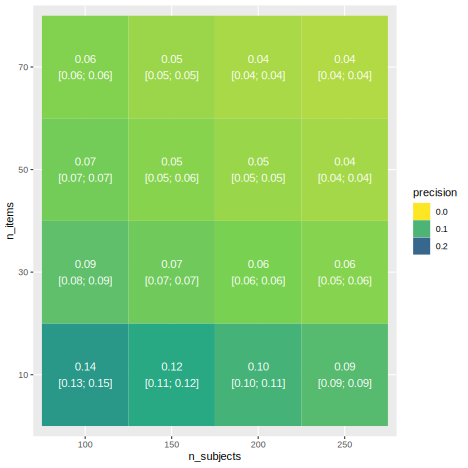
\includegraphics{manuscript_files/figure-pdf/fig-finalprecision-1.pdf}

}

\end{figure}%

As should be the case, precision estimates in
Figure~\ref{fig-finalprecision} increase (i.e., average width of CI
decreases) with the number of included subjects and items. The CIs
reported here indicate how precisely the expected width of the CI for
our focal contrast was estimated by our simulation. Applying our simple
heuristic of targeting an expected CI width that is smaller than 0.1, we
see the same trade-off between the number of subjects and the number of
items as with planning for power. We could either choose 100 subjects
and 30 items or 250 subjects and 10 items. Note that our simple
heuristic for determining sample size in the planning for precision
scenario was quite liberal. This is reflected in the result that we
would need a smaller sample size than in the planning for power
scenario. With a more conservative precision target, the result is
generally the opposite: As a rule, precise parameter estimates usually
require bigger samples than null hypothesis testing.

\subsection{Step 7 (optional): Conduct sensitivity
analysis}\label{step-7-optional-conduct-sensitivity-analysis}

In our case study, we have performed simulation-based sample size
planning from a single set of parameter values that reflect our
assumptions of an expected effect size. Instead of extracting this
expected effect size from meta-analyses or pilot data, which has been
the main focus of previous tutorials (e.g.,
\citeproc{ref-kumleEstimatingPowerGeneralized2021}{Kumle et al., 2021}),
we have demonstrated some strategies to determine plausible parameter
values in GLMMs based on domain knowledge. When sample sizes are chosen
based on the results of our simulation-based power analysis, a future
study will be informative to reject the null hypothesis if an effect of
our \emph{expected size} is present (or estimate the effect with
satisfying precision). However, if the true effect is indeed smaller,
power (or precision) will be lower, and the study might not be
sufficiently informative. A common, more conservative strategy for
sample size justification is to perform sample size planning for the
smallest effect size of interest (SESOI). An effect smaller than the
SESOI would be considered too small to be interesting or practically
meaningful, even if the effect is not actually zero
(\citeproc{ref-kingPointMinimalImportant2011}{King, 2011};
\citeproc{ref-lakensEquivalenceTestingPsychological2018}{Lakens, Scheel,
et al., 2018}). Unfortunately, specifying a plausible SESOI is a
challenging task (for strategies on how to specify a SESOI, see Lakens
(\citeproc{ref-lakensSampleSizeJustification2022}{2022a}), Riesthuis
(\citeproc{ref-riesthuisSimulationBasedPowerAnalyses2024}{2024}), or
Lakens (\citeproc{ref-lakensImprovingYourStatistical2022}{2022b})). When
domain knowledge or formal theories about the research topic of interest
are too vague to specify a meaningful SESOI, it is still recommended to
demonstrate power or precision for different effect sizes in a
\emph{sensitivity power analysis}
(\citeproc{ref-lakensSampleSizeJustification2022}{Lakens, 2022a}). By
simulating power (or precision) for different effect sizes (in addition
to the different number of subjects and items), one can make sure that
power (or precision) would still be sufficient to detect smaller effect
sizes than our expected effect or at least get an impression of how
strongly power (or precision) depends on the size of the true effect.
For our case study that investigates combined hypotheses in a GLMM
modeling framework, sensitivity analysis would require manually
specifying additional sets of plausible parameter values that reflect
scenarios with smaller or larger differences between groups with respect
to our specific research question. Power (or precision) could then be
simulated for several of these scenarios (across different numbers of
subjects and items, as considered earlier). In steps 2 and 4 of the
tutorial, we have briefly discussed scenarios where the applied
statistical model is more (or less) parsimonious than the
data-generating process. Sensitivity analysis can be used to assess the
consequences of a mismatch by investigating different combinations of
data-generating processes and statistical models. Such extended
simulations can be a great resource to make an informed decision about
the concrete model to estimate for the planned study where the true
data-generating process is unknown. Although recommended, we do not
present a sensitivity analysis for our case study to keep the length of
the tutorial manageable.

\section{Conclusion and outlook}\label{conclusion-and-outlook}

In this tutorial, we provided a step-by-step guide on how to perform
tailored simulation-based sample size planning for GLMMs based on a
concrete case study. To conclude, we want to give an outlook on five
developments regarding the future role of simulation-based sample size
planning in experimental research:

\begin{enumerate}
\def\labelenumi{\arabic{enumi}.}
\item
  As experimental designs become more complex and the appropriate
  flexible statistical frameworks, like GLMMs, become more popular,
  there is an ever growing need for simulation-based sample size
  planning in experimental research.
\item
  The ability to conduct simulation-based sample size planning becomes
  an increasingly valuable skill that should be taught to experimental
  researchers. By incorporating such training into research methods
  courses and workshops, researchers can improve the quality of their
  experimental designs and enhance the rigor of their studies. The need
  to reason about how to simulate plausible data that is in line with
  the research hypothesis, while not violating domain expertise on how
  plausible data should look, might also contribute to planning more
  insightful studies that can answer more precise research questions
  (\citeproc{ref-yarkoniGeneralizabilityCrisis2022}{Yarkoni, 2022}).
\item
  Given the significant disconnect between the amount of effort required
  to perform tailored simulation-based sample size planning and the
  perceived effort estimated by researchers and collaborators in
  experimental research, there is a need to address the mismatch in
  effort perception. Many researchers request simulation-based power
  analyses from statisticians or methodological experts without fully
  comprehending the complexity and time-consuming nature of these
  tailored simulations. Therefore, it is crucial to raise awareness
  about the effort involved to ensure realistic expectations and
  effective collaboration with methodological experts.
\item
  Tailored data simulations and power analyses are not mere
  technicalities; they are valuable research contributions that deserve
  adequate recognition in experimental research. Their importance can be
  reflected by highlighting the simulation work in a publication or even
  allocating them a separate publication, or incorporating them as a
  significant component of stage 1 preregistered reports
  (\citeproc{ref-chambersPresentFutureRegistered2022}{Chambers \&
  Tzavella, 2022}).
\item
  Simulation-based sample size planning aligns well with the principles
  of Open Science and preregistration and could be further integrated.
  When researchers have access to simulated data based on their
  pre-specified model, analyzing the collected dataset becomes
  straightforward and unambiguous. By preregistering their
  simulation-based sample size plan, researchers enhance the
  transparency and accountability of their experimental procedures,
  contributing to the credibility and reproducibility of research.
\end{enumerate}

\section{References}\label{references}

\phantomsection\label{refs}
\begin{CSLReferences}{1}{0}
\bibitem[\citeproctext]{ref-albersWhenPowerAnalyses2018a}
Albers, C., \& Lakens, D. (2018). When power analyses based on pilot
data are biased: {Inaccurate} effect size estimators and follow-up bias.
\emph{Journal of Experimental Social Psychology}, \emph{74}, 187--195.
\url{https://doi.org/10.1016/j.jesp.2017.09.004}

\bibitem[\citeproctext]{ref-R-marginaleffects}
Arel-Bundock, V., Greifer, N., \& Heiss, A. (Forthcoming). How to
interpret statistical models using {marginaleffects} in {R} and
{Python}. \emph{Journal of Statistical Software}.

\bibitem[\citeproctext]{ref-arendStatisticalPowerTwolevel2019}
Arend, M. G., \& Schäfer, T. (2019). Statistical power in two-level
models: {A} tutorial based on {Monte Carlo} simulation.
\emph{Psychological Methods}, \emph{24}(1), 1--19.
\url{https://doi.org/10.1037/met0000195}

\bibitem[\citeproctext]{ref-batesFittingLinearMixedEffects2015}
Bates, D., Mächler, M., Bolker, B., \& Walker, S. (2015). Fitting
{Linear Mixed-Effects Models Using} {\textbf{Lme4}}. \emph{Journal of
Statistical Software}, \emph{67}(1).
\url{https://doi.org/10.18637/jss.v067.i01}

\bibitem[\citeproctext]{ref-R-RJ-2021-048}
Bengtsson, H. (2021). A unifying framework for parallel and distributed
processing in r using futures. \emph{The R Journal}, \emph{13}(2),
208--227. \url{https://doi.org/10.32614/RJ-2021-048}

\bibitem[\citeproctext]{ref-benjaminRedefineStatisticalSignificance2017}
Benjamin, D. J., Berger, J. O., Johannesson, M., Nosek, B. A.,
Wagenmakers, E.-J., Berk, R., Bollen, K. A., Brembs, B., Brown, L.,
Camerer, C., Cesarini, D., Chambers, C. D., Clyde, M., Cook, T. D., De
Boeck, P., Dienes, Z., Dreber, A., Easwaran, K., Efferson, C., \ldots{}
Johnson, V. E. (2017). Redefine statistical significance. \emph{Nature
Human Behaviour}, \emph{2}(1), 6--10.
\url{https://doi.org/10.1038/s41562-017-0189-z}

\bibitem[\citeproctext]{ref-bocktingSimulationbasedPriorKnowledge2024}
Bockting, F., Radev, S. T., \& Bürkner, P.-C. (2024). Simulation-based
prior knowledge elicitation for parametric {Bayesian} models.
\emph{Scientific Reports}, \emph{14}(1), 17330.
\url{https://doi.org/10.1038/s41598-024-68090-7}

\bibitem[\citeproctext]{ref-bolkerLinearGeneralizedLinear2015}
Bolker, B. M. (2015). Linear and generalized linear mixed models. In G.
A. Fox, S. Negrete-Yankelevich, \& V. J. Sosa (Eds.), \emph{Ecological
{Statistics}} (1st ed., pp. 309--333). Oxford University PressOxford.
\url{https://doi.org/10.1093/acprof:oso/9780199672547.003.0014}

\bibitem[\citeproctext]{ref-brooksGlmmTMBBalancesSpeed2017}
Brooks, M., E., Kristensen, K., Benthem, van, J., Magnusson, A., Berg,
C., W., Nielsen, A., Skaug, H., J., Mächler, M., \& Bolker, B., M.
(2017). {glmmTMB Balances Speed} and {Flexibility Among Packages} for
{Zero-inflated Generalized Linear Mixed Modeling}. \emph{The R Journal},
\emph{9}(2), 378. \url{https://doi.org/10.32614/RJ-2017-066}

\bibitem[\citeproctext]{ref-brownIntroductionLinearMixedEffects2021}
Brown, V. A. (2021). An {Introduction} to {Linear Mixed-Effects
Modeling} in {R}. \emph{Advances in Methods and Practices in
Psychological Science}, \emph{4}(1), 2515245920960351.
\url{https://doi.org/10.1177/2515245920960351}

\bibitem[\citeproctext]{ref-brysbaertPowerAnalysisEffect2018}
Brysbaert, M., \& Stevens, M. (2018). Power {Analysis} and {Effect Size}
in {Mixed Effects Models}: {A Tutorial}. \emph{Journal of Cognition},
\emph{1}(1), 9. \url{https://doi.org/10.5334/joc.10}

\bibitem[\citeproctext]{ref-burknerBrmsPackageBayesian2017}
Bürkner, P.-C. (2017). Brms: {An R Package} for {Bayesian Multilevel
Models Using Stan}. \emph{Journal of Statistical Software}, \emph{80},
1--28. \url{https://doi.org/10.18637/jss.v080.i01}

\bibitem[\citeproctext]{ref-burknerAdvancedBayesianMultilevel2018}
Bürkner, P.-C. (2018). Advanced {Bayesian Multilevel Modeling} with the
{R Package} brms. \emph{The R Journal}, \emph{10}(1), 395.
\url{https://doi.org/10.32614/RJ-2018-017}

\bibitem[\citeproctext]{ref-buttonPowerFailureWhy2013}
Button, K. S., Ioannidis, J. P. A., Mokrysz, C., Nosek, B. A., Flint,
J., Robinson, E. S. J., \& Munafò, M. R. (2013). Power failure: Why
small sample size undermines the reliability of neuroscience.
\emph{Nature Reviews Neuroscience}, \emph{14}(5), 365--376.
\url{https://doi.org/10.1038/nrn3475}

\bibitem[\citeproctext]{ref-camererEvaluatingReplicabilitySocial2018}
Camerer, C. F., Dreber, A., Holzmeister, F., Ho, T.-H., Huber, J.,
Johannesson, M., Kirchler, M., Nave, G., Nosek, B. A., Pfeiffer, T.,
Altmejd, A., Buttrick, N., Chan, T., Chen, Y., Forsell, E., Gampa, A.,
Heikensten, E., Hummer, L., Imai, T., \ldots{} Wu, H. (2018). Evaluating
the replicability of social science experiments in {Nature} and
{Science} between 2010 and 2015. \emph{Nature Human Behaviour},
\emph{2}(9), 637--644. \url{https://doi.org/10.1038/s41562-018-0399-z}

\bibitem[\citeproctext]{ref-chambersPresentFutureRegistered2022}
Chambers, C. D., \& Tzavella, L. (2022). The past, present and future of
{Registered Reports}. \emph{Nature Human Behaviour}, \emph{6}(1),
29--42. \url{https://doi.org/10.1038/s41562-021-01193-7}

\bibitem[\citeproctext]{ref-R-pwr}
Champely, S. (2020). \emph{Pwr: Basic functions for power analysis}.
\url{https://github.com/heliosdrm/pwr}

\bibitem[\citeproctext]{ref-cohenPowerPrimer1992}
Cohen, J. (1992). A power primer. \emph{Psychological Bulletin},
\emph{112}(1), 155--159.
\url{https://doi.org/10.1037/0033-2909.112.1.155}

\bibitem[\citeproctext]{ref-cummingNewStatisticsWhy2014}
Cumming, G. (2014). The {New Statistics}: {Why} and {How}.
\emph{Psychological Science}, \emph{25}(1), 7--29.
\url{https://doi.org/10.1177/0956797613504966}

\bibitem[\citeproctext]{ref-R-faux}
DeBruine, L. (2023). \emph{Faux: Simulation for factorial designs}.
Zenodo. \url{https://doi.org/10.5281/zenodo.2669586}

\bibitem[\citeproctext]{ref-debruineUnderstandingMixedEffectsModels2021}
DeBruine, L., \& Barr, D. J. (2021). Understanding {Mixed-Effects Models
Through Data Simulation}. \emph{Advances in Methods and Practices in
Psychological Science}, \emph{4}(1), 2515245920965119.
\url{https://doi.org/10.1177/2515245920965119}

\bibitem[\citeproctext]{ref-deffnerCausalFrameworkCrossCultural2022}
Deffner, D., Rohrer, J. M., \& McElreath, R. (2022). A {Causal
Framework} for {Cross-Cultural Generalizability}. \emph{Advances in
Methods and Practices in Psychological Science}, \emph{5}(3),
251524592211063. \url{https://doi.org/10.1177/25152459221106366}

\bibitem[\citeproctext]{ref-dmitrienkoTraditionalMultiplicityAdjustment2013}
Dmitrienko, A., \& D'Agostino, R. (2013). Traditional multiplicity
adjustment methods in clinical trials. \emph{Statistics in Medicine},
\emph{32}(29), 5172--5218. \url{https://doi.org/10.1002/sim.5990}

\bibitem[\citeproctext]{ref-ebersoleManyLabsTesting2020}
Ebersole, C. R., Mathur, M. B., Baranski, E., Bart-Plange, D.-J.,
Buttrick, N. R., Chartier, C. R., Corker, K. S., Corley, M., Hartshorne,
J. K., IJzerman, H., Lazarević, L. B., Rabagliati, H., Ropovik, I.,
Aczel, B., Aeschbach, L. F., Andrighetto, L., Arnal, J. D., Arrow, H.,
Babincak, P., \ldots{} Nosek, B. A. (2020). Many {Labs} 5: {Testing
Pre-Data-Collection Peer Review} as an {Intervention} to {Increase
Replicability}. \emph{Advances in Methods and Practices in Psychological
Science}, \emph{3}(3), 309--331.
\url{https://doi.org/10.1177/2515245920958687}

\bibitem[\citeproctext]{ref-endersSimpleMonteCarlo2023}
Enders, C. K., Keller, B. T., \& Woller, M. P. (2023). A simple {Monte
Carlo} method for estimating power in multilevel designs.
\emph{Psychological Methods}. \url{https://doi.org/10.1037/met0000614}

\bibitem[\citeproctext]{ref-fahrmeirRegressionModelsMethods2021}
Fahrmeir, L., Kneib, T., Lang, S., \& Marx, B. D. (2021).
\emph{Regression: {Models}, {Methods} and {Applications}}. Springer
Berlin Heidelberg. \url{https://doi.org/10.1007/978-3-662-63882-8}

\bibitem[\citeproctext]{ref-gelmanBayesianWorkflow2020}
Gelman, A., Vehtari, A., Simpson, D., Margossian, C. C., Carpenter, B.,
Yao, Y., Kennedy, L., Gabry, J., Bürkner, P.-C., \& Modrák, M. (2020).
\emph{Bayesian {Workflow}} (arXiv:2011.01808). arXiv.
\url{https://arxiv.org/abs/2011.01808}

\bibitem[\citeproctext]{ref-gomilaMissingDataExperiments2022}
Gomila, R., \& Clark, C. S. (2022). Missing data in experiments:
{Challenges} and solutions. \emph{Psychological Methods}, \emph{27}(2),
143--155. \url{https://doi.org/10.1037/met0000361}

\bibitem[\citeproctext]{ref-greenSIMRPackagePower2016}
Green, P., \& MacLeod, C. J. (2016). {SIMR}: An {R} package for power
analysis of generalized linear mixed models by simulation. \emph{Methods
in Ecology and Evolution}, \emph{7}(4), 493--498.
\url{https://doi.org/10.1111/2041-210X.12504}

\bibitem[\citeproctext]{ref-hallgrenConductingSimulationStudies2013}
Hallgren, K. A. (2013). Conducting {Simulation Studies} in the {R
Programming Environment}. \emph{Tutorials in Quantitative Methods for
Psychology}, \emph{9}(2), 43--60.
\url{https://doi.org/10.20982/tqmp.09.2.p043}

\bibitem[\citeproctext]{ref-hartmannFlexiblePriorElicitation2020}
Hartmann, M., Agiashvili, G., Bürkner, P., \& Klami, A. (2020). Flexible
prior elicitation via the prior predictive distribution. In J. Peters \&
D. Sontag (Eds.), \emph{Proceedings of the 36th conference on
uncertainty in artificial intelligence ({UAI})} (Vol. 124, pp.
1129--1138). PMLR.

\bibitem[\citeproctext]{ref-iddiPowerSampleSize2022}
Iddi, S., \& Donohue, M. C. (2022). Power and {Sample Size} for
{Longitudinal Models} in {R} -- {The} longpower {Package} and {Shiny
App}. \emph{The R Journal}, \emph{14}(1), 264--282.
\url{https://doi.org/10.32614/RJ-2022-022}

\bibitem[\citeproctext]{ref-johnsonPowerAnalysisGeneralized2015}
Johnson, P. C. D., Barry, S. J. E., Ferguson, H. M., \& Müller, P.
(2015). Power analysis for generalized linear mixed models in ecology
and evolution. \emph{Methods in Ecology and Evolution}, \emph{6}(2),
133--142. \url{https://doi.org/10.1111/2041-210X.12306}

\bibitem[\citeproctext]{ref-kainPracticalGuidePower2015}
Kain, M. P., Bolker, B. M., \& McCoy, M. W. (2015). A practical guide
and power analysis for {GLMMs}: Detecting among treatment variation in
random effects. \emph{PeerJ}, \emph{3}, e1226.
\url{https://doi.org/10.7717/peerj.1226}

\bibitem[\citeproctext]{ref-kelleySampleSizePlanning2006}
Kelley, K., \& Rausch, J. R. (2006). Sample size planning for the
standardized mean difference: {Accuracy} in parameter estimation via
narrow confidence intervals. \emph{Psychological Methods}, \emph{11}(4),
363--385. \url{https://doi.org/10.1037/1082-989X.11.4.363}

\bibitem[\citeproctext]{ref-kingPointMinimalImportant2011}
King, M. T. (2011). A point of minimal important difference ({MID}): A
critique of terminology and methods. \emph{Expert Review of
Pharmacoeconomics \& Outcomes Research}, \emph{11}(2), 171--184.
\url{https://doi.org/10.1586/erp.11.9}

\bibitem[\citeproctext]{ref-kruschkeBayesianNewStatistics2018}
Kruschke, J. K., \& Liddell, T. M. (2018). The {Bayesian New
Statistics}: {Hypothesis} testing, estimation, meta-analysis, and power
analysis from a {Bayesian} perspective. \emph{Psychonomic Bulletin \&
Review}, \emph{25}(1), 178--206.
\url{https://doi.org/10.3758/s13423-016-1221-4}

\bibitem[\citeproctext]{ref-kumleEstimatingPowerGeneralized2021}
Kumle, L., Võ, M. L.-H., \& Draschkow, D. (2021). Estimating power in
(generalized) linear mixed models: {An} open introduction and tutorial
in {R}. \emph{Behavior Research Methods}, \emph{53}(6), 2528--2543.
\url{https://doi.org/10.3758/s13428-021-01546-0}

\bibitem[\citeproctext]{ref-lafitSelectionNumberParticipants2021}
Lafit, G., Adolf, J. K., Dejonckheere, E., Myin-Germeys, I.,
Viechtbauer, W., \& Ceulemans, E. (2021). Selection of the {Number} of
{Participants} in {Intensive Longitudinal Studies}: {A User-Friendly
Shiny App} and {Tutorial} for {Performing Power Analysis} in {Multilevel
Regression Models That Account} for {Temporal Dependencies}.
\emph{Advances in Methods and Practices in Psychological Science},
\emph{4}(1), 251524592097873.
\url{https://doi.org/10.1177/2515245920978738}

\bibitem[\citeproctext]{ref-lakensSampleSizeJustification2022}
Lakens, D. (2022a). Sample {Size Justification}. \emph{Collabra:
Psychology}, \emph{8}(1), 33267.
\url{https://doi.org/10.1525/collabra.33267}

\bibitem[\citeproctext]{ref-lakensImprovingYourStatistical2022}
Lakens, D. (2022b). \emph{Improving {Your Statistical Inferences}}.
Zenodo. \url{https://doi.org/10.5281/ZENODO.6409077}

\bibitem[\citeproctext]{ref-lakensJustifyYourAlpha2018}
Lakens, D., Adolfi, F. G., Albers, C. J., Anvari, F., Apps, M. A. J.,
Argamon, S. E., Baguley, T., Becker, R. B., Benning, S. D., Bradford, D.
E., Buchanan, E. M., Caldwell, A. R., Van Calster, B., Carlsson, R.,
Chen, S.-C., Chung, B., Colling, L. J., Collins, G. S., Crook, Z.,
\ldots{} Zwaan, R. A. (2018). Justify your alpha. \emph{Nature Human
Behaviour}, \emph{2}(3), 168--171.
\url{https://doi.org/10.1038/s41562-018-0311-x}

\bibitem[\citeproctext]{ref-lakensSimulationBasedPowerAnalysis2021}
Lakens, D., \& Caldwell, A. R. (2021). Simulation-{Based Power Analysis}
for {Factorial Analysis} of {Variance Designs}. \emph{Advances in
Methods and Practices in Psychological Science}, \emph{4}(1),
251524592095150. \url{https://doi.org/10.1177/2515245920951503}

\bibitem[\citeproctext]{ref-lakensEquivalenceTestingPsychological2018}
Lakens, D., Scheel, A. M., \& Isager, P. M. (2018). Equivalence
{Testing} for {Psychological Research}: {A Tutorial}. \emph{Advances in
Methods and Practices in Psychological Science}, \emph{1}(2), 259--269.
\url{https://doi.org/10.1177/2515245918770963}

\bibitem[\citeproctext]{ref-lanePowerStrugglesEstimating2018}
Lane, S. P., \& Hennes, E. P. (2018). Power struggles: {Estimating}
sample size for multilevel relationships research. \emph{Journal of
Social and Personal Relationships}, \emph{35}(1), 7--31.
\url{https://doi.org/10.1177/0265407517710342}

\bibitem[\citeproctext]{ref-lebeauPowerAnalysisSimulation2019}
LeBeau, B. (2019). \emph{Power {Analysis} by {Simulation} using {R} and
simglm}. \url{https://doi.org/10.17077/f7kk-6w7f}

\bibitem[\citeproctext]{ref-leeUsingTidyversePackage2020}
Lee, S., Sriutaisuk, S., \& Kim, H. (2020). Using the {Tidyverse
Package} in {R} for {Simulation Studies} in {SEM}. \emph{Structural
Equation Modeling: A Multidisciplinary Journal}, \emph{27}(3), 468--482.
\url{https://doi.org/10.1080/10705511.2019.1644515}

\bibitem[\citeproctext]{ref-littleStatisticalAnalysisMissing2014}
Little, R. J. A., \& Rubin, D. B. (2014). \emph{Statistical {Analysis}
with {Missing Data}} (2nd ed). Wiley.

\bibitem[\citeproctext]{ref-lundbergWhatYourEstimand2021}
Lundberg, I., Johnson, R., \& Stewart, B. M. (2021). What {Is Your
Estimand}? {Defining} the {Target Quantity Connects Statistical
Evidence} to {Theory}. \emph{American Sociological Review},
\emph{86}(3), 532--565. \url{https://doi.org/10.1177/00031224211004187}

\bibitem[\citeproctext]{ref-magnussonConsequencesIgnoringTherapist2018}
Magnusson, K., Andersson, G., \& Carlbring, P. (2018). The consequences
of ignoring therapist effects in trials with longitudinal data: {A}
simulation study. \emph{Journal of Consulting and Clinical Psychology},
\emph{86}(9), 711--725. \url{https://doi.org/10.1037/ccp0000333}

\bibitem[\citeproctext]{ref-martinMeasuringIndividualDifferences2011}
Martin, J. G. A., Nussey, D. H., Wilson, A. J., \& Réale, D. (2011).
Measuring individual differences in reaction norms in field and
experimental studies: A power analysis of random regression models.
\emph{Methods in Ecology and Evolution}, \emph{2}(4), 362--374.
\url{https://doi.org/10.1111/j.2041-210X.2010.00084.x}

\bibitem[\citeproctext]{ref-matuschekBalancingTypeError2017}
Matuschek, H., Kliegl, R., Vasishth, S., Baayen, H., \& Bates, D.
(2017). Balancing {Type I} error and power in linear mixed models.
\emph{Journal of Memory and Language}, \emph{94}, 305--315.
\url{https://doi.org/10.1016/j.jml.2017.01.001}

\bibitem[\citeproctext]{ref-maxwellSampleSizePlanning2008}
Maxwell, S. E., Kelley, K., \& Rausch, J. R. (2008). Sample {Size
Planning} for {Statistical Power} and {Accuracy} in {Parameter
Estimation}. \emph{Annual Review of Psychology}, \emph{59}(1), 537--563.
\url{https://doi.org/10.1146/annurev.psych.59.103006.093735}

\bibitem[\citeproctext]{ref-mcelreathStatisticalRethinkingBayesian2020}
McElreath, R. (2020). \emph{Statistical {Rethinking}: {A Bayesian
Course} with {Examples} in {R} and {Stan}} (2nd ed.). {Chapman and
Hall/CRC}. \url{https://doi.org/10.1201/9780429029608}

\bibitem[\citeproctext]{ref-meteyardBestPracticeGuidance2020a}
Meteyard, L., \& Davies, R. A. I. (2020). Best practice guidance for
linear mixed-effects models in psychological science. \emph{Journal of
Memory and Language}, \emph{112}, 104092.
\url{https://doi.org/10.1016/j.jml.2020.104092}

\bibitem[\citeproctext]{ref-mikkolaPriorKnowledgeElicitation2023}
Mikkola, P., Martin, O. A., Chandramouli, S., Hartmann, M., Abril Pla,
O., Thomas, O., Pesonen, H., Corander, J., Vehtari, A., Kaski, S.,
Bürkner, P.-C., \& Klami, A. (2023). Prior {Knowledge Elicitation}: {The
Past}, {Present}, and {Future}. \emph{Bayesian Analysis}, \emph{-1}(-1).
\url{https://doi.org/10.1214/23-BA1381}

\bibitem[\citeproctext]{ref-murayamaSummarystatisticsbasedPowerAnalysis2022}
Murayama, K., Usami, S., \& Sakaki, M. (2022). Summary-statistics-based
power analysis: {A} new and practical method to determine sample size
for mixed-effects modeling. \emph{Psychological Methods}.
\url{https://doi.org/10.1037/met0000330}

\bibitem[\citeproctext]{ref-preacherComputationalToolsProbing2006}
Preacher, K. J., Curran, P. J., \& Bauer, D. J. (2006). Computational
{Tools} for {Probing Interactions} in {Multiple Linear Regression},
{Multilevel Modeling}, and {Latent Curve Analysis}. \emph{Journal of
Educational and Behavioral Statistics}, \emph{31}(4), 437--448.
\url{https://doi.org/10.3102/10769986031004437}

\bibitem[\citeproctext]{ref-R-base}
R Core Team. (2024). \emph{R: A language and environment for statistical
computing}. R Foundation for Statistical Computing.
\url{https://www.R-project.org/}

\bibitem[\citeproctext]{ref-riesthuisSimulationBasedPowerAnalyses2024}
Riesthuis, P. (2024). Simulation-{Based Power Analyses} for the
{Smallest Effect Size} of {Interest}: {A Confidence-Interval Approach}
for {Minimum-Effect} and {Equivalence Testing}. \emph{Advances in
Methods and Practices in Psychological Science}, \emph{7}(2),
25152459241240722. \url{https://doi.org/10.1177/25152459241240722}

\bibitem[\citeproctext]{ref-schadPrincipledBayesianWorkflow2021}
Schad, D. J., Betancourt, M., \& Vasishth, S. (2021). Toward a
principled {Bayesian} workflow in cognitive science. \emph{Psychological
Methods}, \emph{26}(1), 103--126.
\url{https://doi.org/10.1037/met0000275}

\bibitem[\citeproctext]{ref-schadHowCapitalizePriori2020}
Schad, D. J., Vasishth, S., Hohenstein, S., \& Kliegl, R. (2020). How to
capitalize on a priori contrasts in linear (mixed) models: {A} tutorial.
\emph{Journal of Memory and Language}, \emph{110}, 104038.
\url{https://doi.org/10.1016/j.jml.2019.104038}

\bibitem[\citeproctext]{ref-stefanPracticalChallengesMethodological2022}
Stefan, A. M., Evans, N. J., \& Wagenmakers, E.-J. (2022). Practical
challenges and methodological flexibility in prior elicitation.
\emph{Psychological Methods}, \emph{27}(2), 177--197.
\url{https://doi.org/10.1037/met0000354}

\bibitem[\citeproctext]{ref-uyguntuncEpistemicPragmaticFunction2023}
Uygun Tunç, D., Tunç, M. N., \& Lakens, D. (2023). The epistemic and
pragmatic function of dichotomous claims based on statistical hypothesis
tests. \emph{Theory \& Psychology}, \emph{33}(3), 403--423.
\url{https://doi.org/10.1177/09593543231160112}

\bibitem[\citeproctext]{ref-R-furrr}
Vaughan, D., \& Dancho, M. (2022). \emph{Furrr: Apply mapping functions
in parallel using futures}.
\url{https://CRAN.R-project.org/package=furrr}

\bibitem[\citeproctext]{ref-watsonGeneralisedLinearMixed2023}
Watson, S. I. (2023). \emph{Generalised {Linear Mixed Model
Specification}, {Analysis}, {Fitting}, and {Optimal Design} in {R} with
the glmmr {Packages}}. arXiv.
\url{https://doi.org/10.48550/ARXIV.2303.12657}

\bibitem[\citeproctext]{ref-westfallStatisticalPowerOptimal2014}
Westfall, J., Kenny, D. A., \& Judd, C. M. (2014). Statistical power and
optimal design in experiments in which samples of participants respond
to samples of stimuli. \emph{Journal of Experimental Psychology:
General}, \emph{143}, 2020--2045.
\url{https://doi.org/10.1037/xge0000014}

\bibitem[\citeproctext]{ref-wickhamWelcomeTidyverse2019}
Wickham, H., Averick, M., Bryan, J., Chang, W., McGowan, L., François,
R., Grolemund, G., Hayes, A., Henry, L., Hester, J., Kuhn, M., Pedersen,
T., Miller, E., Bache, S., Müller, K., Ooms, J., Robinson, D., Seidel,
D., Spinu, V., \ldots{} Yutani, H. (2019). Welcome to the {Tidyverse}.
\emph{Journal of Open Source Software}, \emph{4}(43), 1686.
\url{https://doi.org/10.21105/joss.01686}

\bibitem[\citeproctext]{ref-wickhamDataScienceImport2023}
Wickham, H., Çetinkaya-Rundel, M., \& Grolemund, G. (2023). \emph{R for
data science: Import, tidy, transform, visualize, and model data} (2nd
edition). O'Reilly.

\bibitem[\citeproctext]{ref-yarkoniGeneralizabilityCrisis2022}
Yarkoni, T. (2022). The generalizability crisis. \emph{Behavioral and
Brain Sciences}, \emph{45}, e1.
\url{https://doi.org/10.1017/S0140525X20001685}

\bibitem[\citeproctext]{ref-yuPassLmePower2019}
Yu, M. (2019). \emph{Pass.lme: {Power} and {Sample Size} for {Linear
Mixed Effect Models}} (p. 0.9.0). Comprehensive R Archive Network.
\url{https://doi.org/10.32614/CRAN.package.pass.lme}

\bibitem[\citeproctext]{ref-zhangPracticalStatisticalPower2018}
Zhang, Z., \& Yuan, K.-H. (2018). \emph{Practical statistical power
analysis using {Webpower} and {R}}. ISDSA Press.
\url{https://doi.org/10.35566/power}

\bibitem[\citeproctext]{ref-zimmerSampleSizePlanning2023}
Zimmer, F., Henninger, M., \& Debelak, R. (2023). Sample size planning
for complex study designs: {A} tutorial for the mlpwr package.
\emph{Behavior Research Methods}.
\url{https://doi.org/10.3758/s13428-023-02269-0}

\end{CSLReferences}






\end{document}
